%%%%%%%%%%%%%%%%%%%%%%%%%%%%%%%%%%%%%%%%%
% Journal Article
% LaTeX Template
% Version 2.0 (February 7, 2023)
%
% This template originates from:
% https://www.LaTeXTemplates.com
%
% Author:
% Vel (vel@latextemplates.com)
%
% License:
% CC BY-NC-SA 4.0 (https://creativecommons.org/licenses/by-nc-sa/4.0/)
%
% NOTE: The bibliography needs to be compiled using the biber engine.
%
%%%%%%%%%%%%%%%%%%%%%%%%%%%%%%%%%%%%%%%%%

%----------------------------------------------------------------------------------------
%	PACKAGES AND OTHER DOCUMENT CONFIGURATIONS
%----------------------------------------------------------------------------------------

\documentclass[
	a4paper, % Paper size, use either a4paper or letterpaper
	10pt, % Default font size, can also use 11pt or 12pt, although this is not recommended
	unnumberedsections, % Comment to enable section numbering
	twoside, % Two side traditional mode where headers and footers change between odd and even pages, comment this option to make them fixed
]{LTJournalArticle}

\usepackage{amsmath} % for \bm command
\usepackage{blkarray} % for blockarray environment
\usepackage{graphicx} % for resizebox command
\usepackage{bm} % for bold math symbols
\usepackage{float} % Add this line to include the float package
\usepackage{colortbl}
\usepackage{geometry} % Adjust margins
\usepackage{booktabs} % For better horizontal rules in tables
\usepackage{pdflscape} % For landscape orientation of the page
\usepackage{longtable}
\usepackage{booktabs}
\usepackage{afterpage}
\usepackage{threeparttable}
\usepackage{tabularx}
\usepackage{caption}
\usepackage{float} % Required for the H option
\usepackage[usenames,dvipsnames]{xcolor}
\usepackage{hyperref}
\usepackage{multicol}

\hypersetup{
    colorlinks = true,
    linkcolor = black,
    anchorcolor = black,
    citecolor = black,
    filecolor = black,
    urlcolor = MidnightBlue
    }

\addbibresource{article.bib} % BibLaTeX bibliography file

\runninghead{Exploring Pig Development with Methylation Networks} % A shortened article title to appear in the running head, leave this command empty for no running head

\footertext{\textit{}} % Text to appear in the footer, leave this command empty for no footer text

\setcounter{page}{1} % The page number of the first page, set this to a higher number if the article is to be part of an issue or larger work

%----------------------------------------------------------------------------------------
%	TITLE SECTION
%----------------------------------------------------------------------------------------
\title{\normalsize Exploring Methylation Dynamics Guiding Pig Fetal Development \\ Using Joint Fused Ridge Estimated Networks} % Article title, use manual lines breaks (\\) to beautify the layout

% Authors are listed in a comma-separated list with superscript numbers indicating affiliations
% \thanks{} is used for any text that should be placed in a footnote on the first page, such as the corresponding author's email, journal acceptance dates, a copyright/license notice, keywords, etc
\author{\small%
	Karolina Wąchała \textsuperscript{1}\thanks{Corresponding author: \href{mailto:karolina.wachaa@wur.nl}{karolina.wachaa@wur.nl}}
}

% Affiliations are output in the \date{} command
\date{\footnotesize\textsuperscript{\textbf{1}}MSc Bioinformatics, Wageningen University \& Research}

\begin{document}

% Additional Title Page
\begin{titlepage}
    \centering
    \vspace*{1cm}
    \hrule % Upper horizontal line
    \vspace{0.2cm}
    {\color{MidnightBlue}\Huge\bfseries Research Practice MAT-79324\par} % Title in dark blue
    \vspace{0.5cm}
    \hrule % Lower horizontal line
    \vspace{0.5cm}
    {\Large Karolina Wąchała, MSc Bioinformatics\par}
    \vfill
    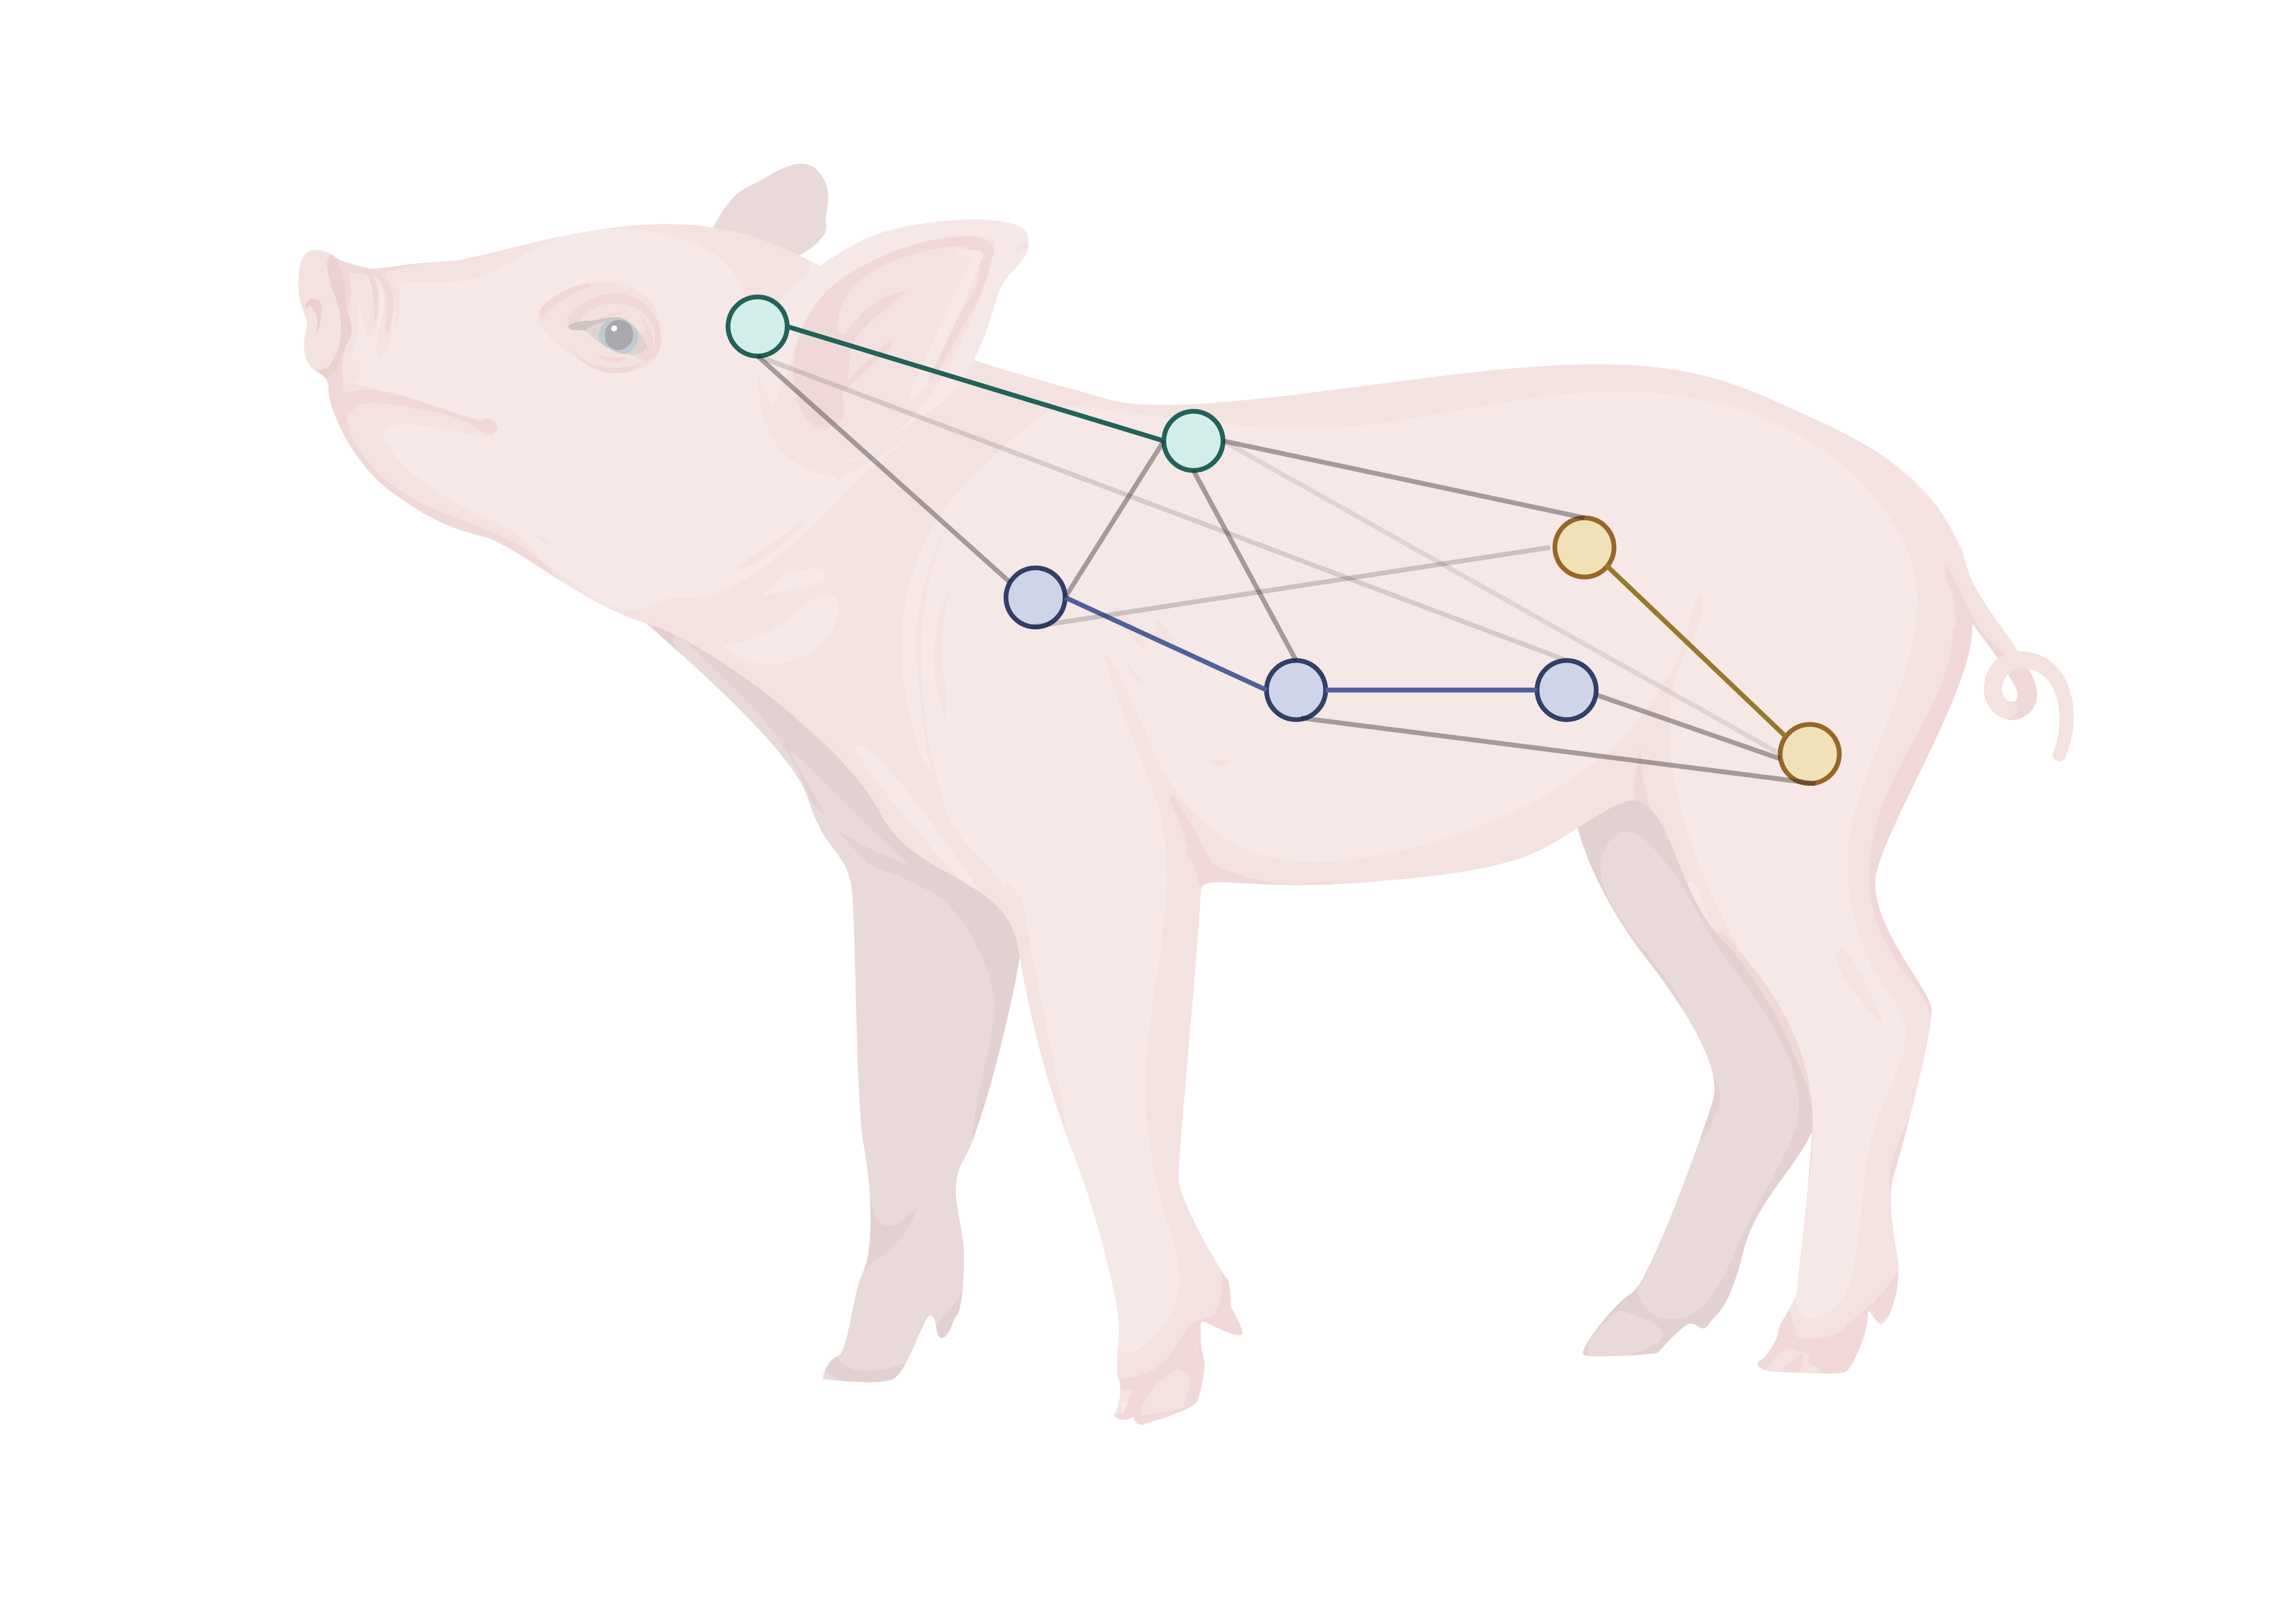
\includegraphics[width=0.95\textwidth]{frontpage.png} % Adjust the width and file name as necessary
    \vfill
    {\large Supervisors: \par} % Add your supervisors' names here
    \vspace{0.5cm} % Additional vertical space
    \textbf{dr. Carel F.W. Peeters}, Mathematical \& Statistical Methods \\
    \textbf{dr. Martijn Derks}, Animal Breeding \& Genomics \\
    \vspace{0.5cm}
    {\large Wageningen University \& Research}\\
	\vspace{0.2cm}
	{\large 11/03/2024}
\end{titlepage}


% Full-width abstract
\onecolumn
\maketitle % Output the title section
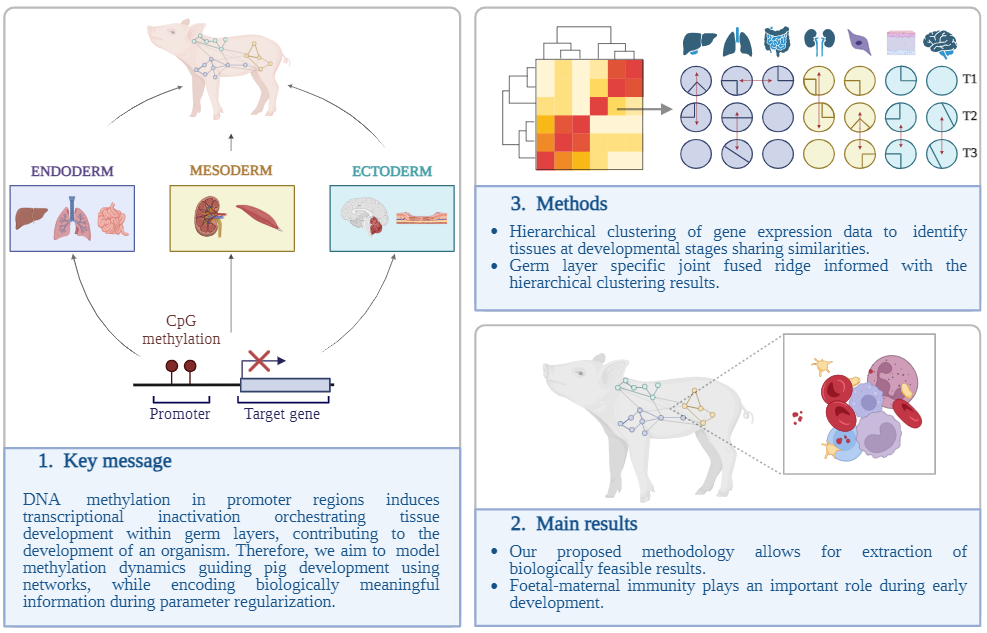
\includegraphics[width=\linewidth]{graphical_abstract.PNG}
\begin{abstract}
    \small
	\noindent \textbf{Background: }Although the organism's genetic information is predominantly 
		  identical among most of its cell types, the expression of the genome is regulated in a 
		  cell type- and context-dependent manner by the epigenome. One of the main epigenetic
		  modifications in mammals is DNA methylation. The DNA methylation in promoter regions 
		  is primarily involved in regulating gene expression by inducing transcriptional inactivation.
		  With the realization that DNA methylation patterns underlying mammalian development are 
		  considerably more dynamic than previously recognized comes the need to implement 
		  methodological approaches of statistical machine learning that allow for capturing 
		  this phenomenon. Therefore, we will explore the feasibility of DNA methylation network 
		  modelling by the joint estimation of regularized precision matrices of time- 
		  and tissue-specific DNA methylation data from the swine genome. 
		  For that, we will use the data spanning seven 
		  swine tissues at three developmental stages: early organogenesis, late organogenesis, 
		  and newborn.\\
		  \textbf{Results: }We were able to show that (1) Utilizing RNA-Seq hierarchical clustering
		  results to control skrinkage is a feasible
		  approach to incorporate biologically meaningful information in the penalty structures of
		  time- and tissue-dependent swine DNA methylation networks; and (2) Joint fused ridge
		  regularization procedure allows for the extraction of the relevant data signal
		  in network modelling of DNA methylation data spanning
		  numerous tissues and developmental stages. We focused our analyses on 61, 48 and 
		  74 differentially expressed between developmental stages,
		  CpG methylated at promoter regions genes extracted for endoderm,
		  mesoderm and ectoderm specific tissues respectively.
		  With our analytical framework,
		  we expanded on the existing knowledge of DNA methylation patterns guiding pig 
		  development\\
		  \textbf{Conclusions: }Our results contribute to advancing exploratory analysis methods 
		  for studying organism development using swine as a model 
		  species. Moreover, with our analytical framework we were able to get biologically feasible results, pointing
		  towards the importance of foetal-maternal immunity during early development. These findings have implications for the fields of epigenomics, developmental 
		  biology and computational biology. Furthermore, we expect that the proposed methodology 
		  can be applied to other omics data in the developmental biolofy field, possibly
		  facilitating hypothesis generation for future research.\\
		  
		  \noindent \normalfont \textbf{Keywords: }Computational Biology, Developmental Biology,
		  DNA methylation, Epigenomics, Network Modelling, Pig Development

\end{abstract}
\twocolumn % Switch to two-column layout

%----------------------------------------------------------------------------------------
%	ARTICLE CONTENTS
%----------------------------------------------------------------------------------------
\section{\large Background}
\subsection{\normalsize Significance of swine in biomedical research and livestock systems}
The pig is a crucial large animal model species in various fields, such as 
xenotransplantation and surgical training \autocite{swindle2012a}. It is 
used to study disease conditions owing to its anatomical and physiological 
similarities to humans \autocite{helke2015a}. With swine genomics recognized 
for its importance in biomedical reseach,
efforts to develop complete swine (epi)genome maps have accelerated 
\autocite{gutierrez2015a, prather2013a}. Furthermore, as porcine genome sequences 
became crucial for the uncovering of molecular genetic variants, they have enabled 
research into the genetic control of quantitative traits such as growth, reproduction
and robustness, e.g., resilience to stressors, which are economically and societally 
desirable in livestock systems \autocite{warr2020a, lenoir2022a}.
The interest in genetic control of desirable traits is not surprising as pigs 
hold significance as a crucial global source of meat production \autocite{mcglone2013a}. 
Genomic selection, which utilizes genomic information to predict the genetic potential 
of individual animals for desirable traits, is widely used in animal breeding with 
the aim of genetic improvements of livestock \autocite{werf2013a, johnsson2023a}. 
However, as DNA methylation, among other functional epigenetic data, is pivotal to 
understand the regulatory mechanisms guiding pig development to e.g., predict 
genomic potential, efforts to characterize epigenetic mechanisms underlying porcine 
development are accelerating \autocite{triantaphyllopoulos2016a}.

\subsection{\normalsize Exploring DNA methylation and its role in swine development} 
Epigenetics is a bridge between the organism's genotype and the phenotype. 
Epigenetic modifications influence the phenotype through chemical changes altering 
gene expression 
without changing the base-pairing of a DNA sequence itself \autocite{goldberg2007a}. 
Mammals, with pigs among them, exhibit three main processes of epigenetic regulation: 
(1) DNA methylation; (2) Histone modifications; and (3) Coding and non-coding RNAs. 
Epigenomics relates to the analysis of these processes across numerous genes in a 
cell or an organism \autocite{champroux2018a}. DNA methylation is a crucial epigenetic 
modification of gene regulation essential for mammalian development and 
has been the most extensively investigated process of epigenetic regulation since its 
discovery in 1948 \autocite{villica2021a}. DNA methylation 
controls the transcriptional activity of genes by altering the chromosomal structure, 
DNA conformation, and DNA stability \autocite{wang2018a}.
It occurs via the covalent transfer of methyl group to the C-5 position of the 
cytosine ring of eukaryotic DNA, regulated by a family of DNA methyltransferases (DNMTs), 
namely DNMT3a and DNMT3b \autocite{jin2011a, ito2022a}. 
The DNMT1 enzyme ensures the maintenance of DNA methylation. Upon establishing DNA 
methylation patterns, DNMT enzymes aid the 
continuation of said patterns into succeeding cellular generations. 
Although DNA methylation is usually erased during zygote 
formation, it is subsequently re-established in the embryo upon implementation 
\autocite{jin2011a}. The formation of 5-methylcytosine resulting 
from DNA methylation is essential for normal embryonic development in mammals, 
as it is vital for processes such as genomic 
imprinting, maintenance of X-chromosome inactivation, chromosomal maintenance and 
genomic stability \autocite{champroux2018a, villica2021a, jin2011a}.\newline

In the majority of mammalian somatic cells, the covalent transfer of methyl group 
occurs predominantly at the 
5'—C—phosphate—G—3' (CpG) dinucleotides, with most CpG sites in the genome fully 
methylated. However, gene promoters contain 
CpG islands, which are CpG-rich regions primarily regulating gene transcription. 
Gene promoters are short segments of DNA 
(100–1,000 base pairs) where gene transcription is initiated, and methylation was revealed 
to regulate gene expression by switching-off 
transcription of the corresponding gene \autocite{lim2019a, le2019a}. 
However, the genome's promoters remain generally unmethylated \autocite{mendoza2022a}. 
Nevertheless, due to advancements in the genome-scale mapping of methylation, 
DNA methylation can be studied in various genomic contexts, from 
transcriptional start sites (TSS) through gene bodies to regulatory elements, 
e.g., gene promoters \autocite{lim2019a, jones2012a}. Although 
traditionally, DNA methylation is primarily associated with CpG islands, 
which are specific genomic regions with frequently 
occurring CG dinucleotide, demethylation seems to occur predominantly in DNA regions 
that are not CpG islands, which has led 
to the recognition of DNA methylation as a vastly dynamic process \autocite{jones2012a}. 
The dynamic nature of DNA methylation highlights the 
complexity of this epigenetic regulatory process, its potential impact 
on gene expression, and, consequently, tissue 
growth and morphogenesis during organism development.

\subsection{\normalsize Dynamic epigenomic switches in swine: Integrating network approaches} 
The GENE-SWitCH project, working in cooperation with the Functional Annotation of 
Animal Genomes (FAANG) 
Consortium \autocite{giuffra2019a}, aimed to uncover the dynamic epigenetic switches 
in the functional genome of swine.
Since gene expression, transcripts and regulatory regions differ in a time- and 
tissue-specific manner, a static view of 
the genome and current genome annotation data sets may restrain a deeper understanding 
of gene expression 
and its function in mammalian development \autocite{acloque2022a}. 
Consequently, a statistical approach allowing for the analysis of these complex 
and dynamic data sets is needed. However, epigenomic data are high-dimensional, 
as the variable dimension (genes) exceeds the 
observation dimension (biological replicates) \autocite{mirza2019a}. 
The high dimensionality of the dataset leads to a so-called curse of 
dimensionality \autocite{donoho2000a}. As the number of dimensions in 
a dataset increases, the mathematical problem space increases 
exponentially \autocite{phan2012a}. Therefore, the curse of dimensionality 
increases the computational and mathematical complexity of 
elucidating the epigenomics mechanisms that govern organism development 
\autocite{donoho2000a}. In the past years, researchers developed 
numerous computational methods for conquering the curse of dimensionality 
\autocite{donoho2000a}. One such method is ridge shrinkage \autocite{ogutu2012a}. Ridge 
shrinkage promotes more stable and reliable estimates of model parameters 
\autocite{wieringen-a}. Therefore, it is applicable in omics 
data analyses. Next to ridge regularization, networks have gained popularity 
as a visually appealing and interpretable 
approach for the analysis of molecular mechanisms measured in thousands of 
variables, e.g., genes \autocite{bodein2022a}.

However, combining data from multiple datasets, e.g., pig tissues at developmental 
stages in a network, might 
dilute the unique biology of each sample, leading to an oversimplified representation 
of the dynamic epigenomics landscape 
during organism development. There is a need for a visually appealing and 
interpretable modelling approach, not only to 
extract DNA methylation networks and visualize how they change during organism development, 
but to separate signal from 
noise efficiently in high-dimensional DNA methylation datasets. Therefore, we aim to 
apply a network modelling approach 
utilizing data fusion over time and tissue types. Fusion will allow us to \textit{borrow} 
strength from variables across DNA 
methylation datasets, helping to improve the stability and accuracy of 
generated networks, by promoting the detection of significant 
edges with higher precision \autocite{price-a}. To decide where fusion penalties 
should be applied, we will utilize results from hierarchical 
clustering of RNA sequencing (RNA-Seq) data. Moreover, using ridge shrinkage and 
fusion we will extract the parameters describing network topology 
jointly for all tissues originating from the same somatic germ layer. Furthermore, 
we will visualize differential networks, 
capturing how DNA methylation dynamics change between developmental stages for 
each tissue. With all these steps combined our 
networks will more accurately capture the intricate biological context of the 
GENE-SWitCh RRBS (Reduced Representation Bisulfite 
Sequencing) datasets, allowing us to gain insights into DNA methylation dynamics 
driving pig development.

%------------------------------------------------

\section{\large Methods}
\subsection{\normalsize Initial datasets}
All data used in this paper were collected prior to our research by the GENE-SWitCh 
project funded by  European Union's Horizon 2020 Research 
and Innovation Programme. The RRBS and RNA-Seq data we used is publicly available 
through the \href{https://data.faang.org/projects/GENE-SWitCH}{FAANG data portal}.
RRBS uses methylation-sensitive restriction enzyme digestion on the genomic DNA. 
The fragmented genomic DNA is then treated with bisulphite and sequenced 
\autocite{kalavacharla2017a}. After treatment of 
fragmented genomic DNA with bisulphite, unmethylated cytosine residues are 
converted to uracil and subsequently to thymine during polumerase chain 
reaction (PCR) amplification, 
while 5-methylcytosine residues remain unaffected \autocite{miyata2017a, li2011a}.
GENE-SWitCH has collected the available RRBS and RNA-Seq data from seven porcine 
tissues representative of the three somatic germ layers:

\begin{enumerate}
	\item Endoderm – liver, lung, small intestine;
	\item Mesoderm – kidney, skeletal muscle from hindlimb;
	\item Ectoderm – hindbrain, skin.
\end{enumerate}

\noindent Moreover, the data stem from three developmental stages: 
30 days post-fertilisation (dpf) or early organogenesis, 70dpf or late organogenesis, 
and from newborn piglets (NB). Additionally, at 30dpf, pooling of 
samples (biological replicates) coming from multiple fetuses 
was performed to ensure enough genetic 
material will be available for sequencing. RNA-Seq data collection was followed up by the normalisation 
of read counts and differential expression analysis. 
The RRBS data, RNA-Seq data, and the differential expression analysis results provided by the 
GENE-SWitCh were the starting point for our research.

\subsection{\normalsize Data Preparation}
The GENE-SWitCH project has utilized RRBS to study genome-wide DNA methylation of 
swine at a 
single-nucleotide resolution. Since RRBS enriches for CpG-dense regions while 
using restriction enzymes cutting at specific sites for fragmentation, 
it does not cover non-CpG areas, and CpGs in areas without the enzyme restriction 
site \autocite{kalavacharla2017a, smith2009a}. Therefore, we focused 
on methylation in the CpG-rich promoter regions to ensure proper coverage.
However, the annotation of promoter regions in CpG-methylated genes is not trivial, 
as for meaningful inference the most precise promoter region specification is desirable. 
The results from chromatin immunoprecipitation followed by sequencing 
(ChIP-Seq) served us to that end. This technology uses antibodies specific to a 
DNA-binding protein of interest to identify regulatory regions 
of the genome. In the case of promoter regions, the H3 lysine 4 trimethylation (H3K4me3) 
is a core histone mark used to identify active promoter regions \autocite{nakato2021a}. 
By invesigating the distribution of histone modification signals around TSSs we 
identified the number of base pairs (bp) upstream and downstream of TSSs where 
promoters are most likely to lie. 
We specified that the read distribution peak is around 200bp upstream, and 50bp 
downstream of gene to TSS.
Moreover, we extracted methylation values only for the significantly differentially 
expressed genes (DEGs) between developmental stages, 
as obtained by GENE-SWitCh \autocite{acloque2022a}. We wanted to retain all DEGs between developmental 
stages, therefore we didn't filter on the fold change.
Moreover, we excluded genes located on the X-chromosome from the analyses,
to mitigate potential biases related to sex differences in gene expression 
and methylation.
We extracted methylation values separately for each tissue at developmental stage, 
resulting in 21 files representing 7 pig tissues at 3 developmental stages.\newline

Prior to exploratory analysis, we processed the data further. 
First, since CpG methylation might occur at 
multiple positions in the promoter region of a gene, while numerous genes 
have alternative promoters aiding pre-mRNA splicing \autocite{xin2008a}, we 
recorded the median 
of replicate methylation values per gene; other data, icluding 
genes for which all methylation values were 0, was dropped. Excluding genes that 
exhibited zero methylation values in all replicates ensured the presence 
of between-sample variation. We thereafter 
transposed the resulting data frames, with replicates arranged in rows and 
genes arranged in columns. Secondly, we normalised (mean centred and divided by 
the standard deviation) the columns of the numeric matrices obtained to normalise the 
range of methylation values, which is a crucial step when implementing algorithms 
that calculate distances between data.                                                                                                                  

\subsection{\normalsize Gaussian Graphical Models}
We aimed to visualise networks representing relationships among variables, where 
each variable corresponds to the methylation value of a CpG 
methylated at promoter DEG between developmental stages. Network science 
evolved from graph theory, a mathematical branch exploring relationships 
between pairs of objects \autocite{i2020a}. Therefore, a network is just 
a collection of elements called nodes, linked together by their interactions, 
known as edges \autocite{hastie2009a}. As the presence of an edge between nodes in the network indicates 
a conditional dependency between the variables, we aimed to extract, 
visualize and analyse Gaussian Graphical Models (GGMS) 
using the \texttt{rags2ridges} R package \autocite{peeters2022a}.
GGM is a type of graphical model that captures the pairwise 
relationships among variables, 
based on the assumption that the joint distribution of these variables 
follows a multivariate normal distribution 
\autocite{altenbuchinger2020a}. When we assume multi-normality, 
the nodes in the 
network represent variables that follow a multivariate normal distribution. 
In this context, conditional independence 
between nodes is equivalent to the corresponding partial correlation zero, 
indicating no relationship, and therefore absence of an edge. Consequently,
partial correlation can measure conditional (in)dependence \autocite{cai2022a}, 
which can be formulated as 

\begin{equation} \label{eq:S1}
X \perp Y \mid Z \leftrightarrow p_{XY \cdot Z} = 0
\end{equation}
	
\noindent for conditional independence and

\begin{equation} \label{eq:S2}
X \not\perp Y \mid Z \leftrightarrow p_{XY \cdot Z} \neq 0
\end{equation}

\noindent in the case of conditional dependence, where \( p_{XY \cdot Z} \) 
is a partial correlation 
coefficient denoting the relationship between two random variables, X and Y, 
conditioned on a set 
of random variables Z which possibly explain this association \autocite{altenbuchinger2020a}. 
The parameters of GGMs, i.e., the partial correlations, can be 
estimated by inverting the sample covariance matrix \( \Sigma \) to obtain the 
precision matrix \( \Omega \). 
Let us consider a covariance matrix

\begin{equation} 
    \label{eq:S3}
    \Sigma = 
    \bordermatrix{~ & x & y & z \cr
        x & 2 & 1 & 1 \cr
        y & 1 & 2 & 1 \cr
        z & 1 & 1 & 1 \cr
    },
\end{equation}

\noindent with the inverse covariance matrix (precision matrix) given by

\begin{equation} 
    \label{eq:S4}
    \Omega = \Sigma^{-1} = 
    \bordermatrix{~ & x & y & z \cr
        x & 1 & 0 & -1 \cr
        y & 0 & 1 & -1 \cr
        z & -1 & -1 & 3 \cr
    },
\end{equation}

\noindent such that $\Sigma \times \Omega$ equals the identity matrix $\mathbf{I}$


\begin{equation} 
    \label{eq:S5}
    \Sigma \times \Omega = I = 
    \bordermatrix{~ & x & y & z \cr
        x & 1 & 0 & 0 \cr
        y & 0 & 1 & 0 \cr
        z & 0 & 0 & 1 \cr
	}.
\end{equation}

\noindent The zeros in the precision matrix indicate conditional independence 
of two variables – X and Y, 
conditioned on the third variable Z (or a set of variables). 
Correlation is a normalised covariance 
\autocite{baba2004a}

\begin{equation} \label{eq:S6}
    \rho_{XY} = \frac{\text{cov}(X, Y)}{\sigma_X \sigma_Y},
\end{equation}

\noindent and the inversion of the covariance matrix will yield a 
partial correlation structure between all variables. 
The partial correlation coefficient $\rho_{x_i x_j \cdot \text{rest}}$ 
between $X_i$ and $X_j$ variables of a partial 
correlation matrix, given all other variables, is associated 
with the precision matrix $\Omega = \omega_{ij} = \Sigma^{-1}$ 
such that

\begin{equation} \label{eq:S7}
    \rho_{x_i x_j \cdot \text{rest}} = -\frac{\omega_{ij}}{\sqrt{\omega_{ii} \omega_{jj}}}
\end{equation}

\noindent where a partial correlation matrix entry $\omega_{ij} = 0$ indicates 
a zero partial correlation (absence of an edge in the network).
\autocite{altenbuchinger2020a}.

\subsection{\normalsize The nonparanormal transformation}
However, GGMs assume that the modelled variables 
follow a multivariate normal distribution, i.e., are jointly Gaussian such that 
for a $\mathbf{X} \in \mathsf{\mathbb{R}}^{n \times p}$ where the rows $X_i$, $i=1, \ldots, n$, 
are independently drawn from the same $p$-variate Gaussian distribution 
$\mathcal{N}(\mu, \Sigma)$ \autocite{li2020a}. That assumption is not met when modelling RRBS data, 
since the violation of the normality assumption is frequently observed in the 
methylation data analysis \autocite{li2018a}. This violation originates from the fact 
that methylation values are bounded between 0 and 1, and their variance is usually 
smaller near the boundaries than near the middle of the interval, 
implying the violation of the homoscedasticity assumption \autocite{weinhold2016a}. 
Therefore, methylation values follow a scaled beta distribution. 
If not accounted for, the distribution of the project data would limit the detection
of true positive edges in the networks. 
Consequently, gene methylation
data from each tissue at developmental stage had to be transformed prior to network modelling.\newline

The need for multivariate gaussian distribution between model variables implies a 
requirement for normality in the marginal distributions and 
linearity in all relationships between variables \autocite{epskamp2018a}. To achieve 
that, we transformed RRBS data by estimating the Gaussian copula to relax the 
assumption of normality \autocite{czado2022a}. A copula is a specific instance 
of a multivariate cumulative distribution function characterized by having 
uniform marginal distributions, 
such that in a 2D \((p=2)\) setting the marginal distributions are

\begin{equation} \label{eq:1}
	X_1 \sim \mathcal{N}(0, 1) \quad \text{and} \quad X_2 \sim \mathcal{N}(0, 1).
\end{equation}

\noindent Liu et al. (2009) \autocite{liu2009a} proposed the nonparanormal 
(NPN) transformation, a special case of a Gaussian copula, to incorporate 
non-Gaussian data to overcome the limiting assumption of multivariate normal data. 
In a 2D setting the nonparanormal transformation aims to establish a set of monotonic 
functions \(f_1, f_2\) for a \(2\)-dimensional random 
variable \(X = (X_1, X_2)\) such 
that the set of functions is multivariate normal distributed 
and \(X \sim \text{NPN}(\mu, \Sigma, f)\). This transformation preserves 
the conditional (in)dependence 
structure between the initial, non-Gaussian variables since each 
function \(f_i\) depends solely on the \(X_i\) variable. Therefore, the 
distribution of \(f(X)\) has the 
same factorization as the distribution of \(X\) \autocite{liu2009a}. 
With NPN transformation the uniform marginal distributions (\ref{eq:1}) are 
transformed by a set of functions such that
\(f_1(X_1) = u_1\) and \(f_2(X_2) = u_2\), with the corresponding Gaussian copula

\begin{equation} \label{eq:2}
	C(u_1, \ldots, u_p) = \Phi_{\mu, \Sigma}(\Phi^{-1}(u_1), \ldots, \Phi^{-1}(u_p)),
\end{equation}

\noindent where $\Phi^{-1}$ denotes the inverse normal standard cumulative 
distribution function (CDF), and $\Phi_2$ denotes the CDF of multivariate distribution 
$N\left(\begin{bmatrix}0 \\ 0\end{bmatrix}, \begin{bmatrix}1 & \rho \\ \rho & 1\end{bmatrix}\right)$. 
Here, we provided an explanation for a 2D setting; 
however, the same operation could be easily extended to higher dimensions, 
since the estimation of a nonparanormal transformation is computationally efficient, 
requiring only one pass of $X \in \mathbb{R}^{n \times p}$ \autocite{jiang2022a}. 
Therefore, we implemented the nonparanormal transformation using the 
\texttt{huge} R package, which 
estimates the Gaussian copula by transforming the variables marginally by 
applying smooth, i.e., continuously differentiable, functions \autocite{jiang2022a}. 
We conducted the NPN transformation via shrunken
empirical cumulative distribution function (ECDF), where the parameter values 
are shrunken during transformation. We performed this transformation of methylation values
separately for each tissue at developmental stage. This shrunken estimate helps to reduce the impact 
of extreme observations. Therefore, 
it can be effective in mitigating the impact of extreme values in situations where 
data values are constrained within a specific range, e.g., methylation values 
between 0 and 1. In this setting, we consider values approaching 0 or 1
to be extreme. 

\subsection{\normalsize Hierarchical clustering of RNA-Seq data}\label{clust}
After transforming methylation values separately for each tissue 
at developmental stage, we performed hierarchical clustering of 
genes and samples using RNA-Seq data. Our goal was to visualise the correlation-based 
relationships between samples based on gene expression data, to facilitate the 
construction of penalty matrices guiding joint fused ridge network extraction
from methylation data. To do so, 
we extracted unique Ensembl gene IDs for each tissue-developmental stage 
combination. These genes were then matched with a TPM (transcript 
per million) file provided by GENE-SWitCH to extract the count-based RNA-Seq transcript 
expression levels of only the genes that were CpG methylated at the promoter 
region and differentially expressed between 30-70dpf and 70dpf-NB. Furthermore, we filtered out
genes located on the X-chromosome, ultimately obtaining expression values 
of 2718 unique genes present in all tissues at developmental stages for clustering.
TPM accounts for sequencing 
depth, which is the total number of reads obtained from an RNA-Seq run, and gene 
length \autocite{zhao2021a}. Nevertheless, the expression data needed pre-processing. 
All TPM values 
were log-transformed, such that \(TPM = \log_2(TPM + 1)\), to ensure they are
non-zero allowing normalization prior to clustering. 
Moreover, the RNA-Seq data was scaled per gene.
After log transformation, the distribution of TPM-based gene expression approached 
normal distribution, whereas scaling brought the variables to a comparable scale. 
Correlation-based hierarchical clustering followed. The pairwise similarity 
between genes was computed as the Pearson correlation since the expression data 
was approximately 
normally distributed. However, since scaling was performed on genes, not samples,
we computed the pairwise similarity between samples as the nonparametric Spearman 
correlation. 
Both genes and samples were clustered using complete linkage to create compact, 
distinct clusters. At last, we implemented the average silhouette width (AWS) method 
to choose the optimal number of sample clusters \autocite{batool2021a}. 
A silhouette represents each cluster by comparing cluster tightness and separation, 
illustrating which data points are positioned within 
the assigned cluster and which lie between the clusters \autocite{rousseeuw1987a}. 
AWS is calculated for each data point by measuring its intra-cluster and inter-cluster 
distance, 
with high values indicating better clustering \autocite{batool2021a}. The optimal 
number of clusters was chosen as k = 16, the location of the maximum, indicating tight, 
well-separated clusters. Subsequently, we generated a heatmap illustrating the 
hierarchical clustering of genes and samples based on the preprocessed RNA-Seq data. 

\subsection{\normalsize Network extraction}\label{netextr-meth}
In preparation for network extraction, all methylation matrices obtained after:

\begin{enumerate}
	\item Taking a median of methylation values per gene;
	\item Removing genes with no between-sample variation;
	\item Scaling methylation values per gene;
	\item Implementing NPN transformation,
\end{enumerate}

\noindent were used to obtain an intersection of 
genes that were present in all seven tissues and three 
developmental stages. However, since only one
gene was shared throughout all matrices, germ-layer-specific intersections 
of genes were obtained to allow for network modelling of methylation
dynamic guiding pig foetal development. 
Thereafter, 
the methylation matrices were filtered to contain methylation values of only 
the genes present in the intersection.
In Table \ref{tab:matrices} we provide an overview of the 21 matrices $[3 \text{ tissues} \times 3 \text{ replicates} + 2(2 \text{ tissues} \times 3 \text{ replicates})]$ obtained for further analysis.

\begin{table}[htbp]
	\caption{An overview of the germ layer-specific methylation matrices obtained for downstream analyses}
	\label{tab:matrices}
	\resizebox{\columnwidth}{!}{%
	\begin{tabular}{lccccccc}
	\hline
	\multicolumn{1}{c}{} & \textbf{Liver} & \textbf{Lung} & \textbf{Intestine} & \textbf{Kidney} & \textbf{Muscle} & \textbf{Hindbrain} & \textbf{Skin} \\ \hline
	\textbf{Endoderm} & \cellcolor[HTML]{CFD5E8} & \cellcolor[HTML]{CFD5E8} & \cellcolor[HTML]{CFD5E8} &  &  &  &  \\
	\textbf{Mesoderm} &  &  &  & \cellcolor[HTML]{F0E2B6} & \cellcolor[HTML]{F0E2B6} &  &  \\
	\textbf{Ectoderm} &  &  &  &  &  & \cellcolor[HTML]{D3EEEA} & \cellcolor[HTML]{D3EEEA} \\ \hline
	\end{tabular}%
	}
	\end{table}

\noindent The methylation matrices consisted of:

\begin{itemize} 
    
    \item $n = 3, p = 61$ for endoderm-specific matrices;
    \item $n = 3, p = 48$ for mesoderm-specific matrices;
    \item $n = 3, p = 74$ for ectoderm-specific matrices.
\end{itemize}

\noindent In \nameref{exgenes} we provide an overview of all germ layer specific genes
that we used for network modelling. We will mow outline the procedure to obtain a joint estimation 
of germ layer- and class-specific regularised precision 
matrices.\newline 

First, let $y_{ig}$ denote a realization of a $p$-dimensional random variable 
(methylation value of a gene), for $i=1,\ldots,n_g$ independent observations 
(biological replicates) corresponding to $g=1,\ldots,G$ non-overlapping classes 
(tissues at developmental stages), drawn from a multivariate normal 
distribution $Y_g \sim N_p(0, \Sigma_g)$. 
The parameters of the multivariate 
Gaussian – sample mean vector and sample 
precision matrix $S_g^{-1} = \Omega_g$ can be derived through maximum 
likelihood estimation (MLE).
The multivariate normal log-likelihood parameterized in terms of the precision matrix for 
the joint $\sum_{g=1}^{G} n_g$ data observations is defined by

\begin{equation} \label{eq:3}
	L(\{\Omega_g\}; \{S_g\}) \propto \sum_g n_g \left(\ln|\Omega_g| - \text{tr}(S_g \Omega_g)\right),
\end{equation}
	
\noindent where $\{\Omega_g\}$ and $\{S_g\}$ denote sets $\{\Omega_g\}_{g=1}^{G}$ 
and $\{S_g\}_{g=1}^{G}$ respectively, and the maximum likelihood estimate $\hat{\Omega}_g^{ML} = S_g^{-1}$ 
when $n_g > p$ \autocite{bilgrau2020a, peeters2022a}.

\noindent To derive the parameters of the multivariate Gaussian
through MLE we want to invert the sample covariance matrix $S_g$ to obtain the precision 
matrix $\Omega_g$ for each class $g$ \autocite{peeters2022a}. However, it is 
not possible with 
variables dimension ($p$) exceeding the observation dimension ($n$) 
\autocite{peeters2022a}. In such a case, the covariance matrix does not have 
a full rank since there 
are not enough observations to span the information of the variable dimension, 
and thus, it cannot be inverted. 

\noindent Since the variable dimension (genes) exceeds the observation 
dimension (biological replicates) in our project, a joint fused ridge estimation will allow the sample 
covariance matrix inversion,
while retaining class-specific information \autocite{peeters2022a}. 
Thus we seek to derive MLE adapting 
formula \ref{eq:3} to include the fused $l_2$ given by

\begin{multline} \label{eq:4}
	- \sum_g \frac{\lambda_{gg}}{2} \|\Omega_g - T_g\|_2^2 \\
	+ \sum_{(g_1, g_2)} \frac{\lambda_{g_1 g_2}}{4} \left\|(\Omega_g - T_{g_1}) - (\Omega_g - T_{g_2})\right\|_2^2,
\end{multline}

\noindent where $T_g$ represent class-specific target matrices that can serve 
to incorporate prior information of the network structure by integrating known 
relationships or dependencies between 
variables into the matrix, $\lambda_{gg}$ represent class-specific ridge penalty 
parameters controlling the rate of shrinkage of the unbiased, high 
variance $\Omega_g$ towards the biased, 
low variance $T_g$, and $\lambda_{g_1 g_2}$ denote pair-specific 
fusion penalty parameters controlling the extent of entry-wise 
similarities between $(\Omega_g - T_{g_1})$ and $(\Omega_g - T_{g_2})$ 
to be retained \autocite{bilgrau2020a, peeters2022a}.
Considering the fused ridge penalty in \ref{eq:4}, the maximizing argument 
for a single data class $g$ is defined by Bigrau et al. (2020) \autocite{bilgrau2020a} as:

\begin{multline} \label{eq:5}
	\hat{\Omega}_g(\Lambda, \{\Omega_{g'}\}_{g' \neq g}) = \\
	\left[\lambda_{g} I_p + \frac{1}{4} (S_{g} - \lambda_{g} T_{g})^2 \right]^{1/2} \\
	+ \frac{1}{2} (S_{g} - \lambda_{g} T_{g})^{-1},
\end{multline}

where

\begin{equation} \label{eq:6}
	S_{g} = S_g - \sum_{g' \neq g} \frac{\lambda_{g' g}}{n_g} (\Omega_{g'} - T_{g'}),
	\quad
	T_{g} = T_g,
\end{equation}

and
	
\begin{equation} \label{eq:7}
	\lambda_{g} = \frac{\lambda_{g \bullet}}{n_g},
\end{equation}

\noindent with $\lambda_{g \bullet}$ denoting the sum of entries in the $g$th row or 
column of the penalty matrix $\Lambda$. The penalty matrix $\Lambda$ can store the 
class-specific (ridge) 
and pair-specific (fusion) penalties with $\lambda_{gg}$ along the diagonal 
and $\lambda_{g_1 g_2}$ off-diagonal \autocite{peeters2022a}. Since GGMS are graphs 
representing complex systems, e.g., methylation values of DEGs on a tissue- 
and time-scale, that partially share a common structure across data classes 
while still retaining 
class-specific features, setting uniform class-specific ridge penalties and 
uniform pair-specific fusion penalties is deemed restrictive 
\autocite{bilgrau2020a, tsai2022a}. 
The fused $l_2$-penalized maximum likelihood approach allows 
simultaneous estimation of multiple precision matrices 
from high-dimensional data classes. In the analysis of factorial 
design, such as tissues at developmental stages, 
a more precise regulation of the individual values of ($\lambda_{gg}$) and ($\lambda_{g_1 g_2}$)
is suitable for the analysis \autocite{bilgrau2020a}. 
It can be achieved by, e.g., informing the penalty matrix $\Lambda$ 
with RNA-Seq hierarchical clustering results.\newline

Therefore, we utilized the hierarchical clustering results to inform three separate 
penalty structures, 
such that each data class was assigned a ridge penalty, assuming considerable
differences in 
class-specific methylation patterns. Furthermore, fusion penalties were 
free to be estimated 
for data classes clustering the closest together. Figure providing visualisation of 
hierarchical clustering results will follow in the \nameref{results}
section. Here we 
provide an overview of 
the penalty structures defined for endoderm:

\[
\resizebox{\columnwidth}{!}{%
    $\varLambda^{En} = 
    \begin{blockarray}{*{10}{c}}
     & \mathbf{L30} & \mathbf{L70} & \mathbf{LNB} & \mathbf{Lu30} & \mathbf{Lu70} & \mathbf{LuNB} & \mathbf{I30} & \mathbf{I70} & \mathbf{INB} \\
    \begin{block}{c [ccccccccc]}
    \mathbf{L30} & \lambda_{L30} & \lambda_{L30L70} & 0 & 0 & 0 & 0 & 0 & 0 & 0 \\
    \mathbf{L70} & \lambda_{L30L70} & \lambda_{L70} & 0 & 0 & 0 & 0 & 0 & 0 & 0 \\
    \mathbf{LNB} & 0 & 0 & \lambda_{LNB} & 0 & 0 & 0 & 0 & 0 & 0 \\
    \mathbf{Lu30} & 0 & 0 & 0 & \lambda_{Lu30} & 0 & 0 & \lambda_{Lu30I30} & 0 & 0 \\
    \mathbf{Lu70} & 0 & 0 & 0 & 0 & \lambda_{Lu70} & \lambda_{Lu70LuNB} & 0 & 0 & 0 \\
    \mathbf{LuNB} & 0 & 0 & 0 & 0 & \lambda_{Lu70LuNB} & \lambda_{LuNB} & 0 & 0 & 0 \\
    \mathbf{I30} & 0 & 0 & 0 & \lambda_{Lu30I30} & 0 & 0 & \lambda_{I30} & 0 & 0 \\
    \mathbf{I70} & 0 & 0 & 0 & 0 & 0 & 0 & 0 & \lambda_{I70} & \lambda_{I70INB} \\
    \mathbf{INB} & 0 & 0 & 0 & 0 & 0 & 0 & 0 & \lambda_{I70INB} & \lambda_{INB} \\
    \end{block}
    \end{blockarray}$};
\]

\noindent mesoderm:

\[
\resizebox{\columnwidth}{!}{
	$\varLambda^{Me} = 
    \begin{blockarray}{l*{6}{c}}
     & \mathbf{K30} & \mathbf{K70} & \mathbf{KNB} & \mathbf{M30} & \mathbf{M70} & \mathbf{MNB} \\
    \begin{block}{l[cccccc]}
    \mathbf{K30} & \lambda_{K30} & \lambda_{K30K70} & 0 & 0 & 0 & 0 \\
    \mathbf{K70} & \lambda_{K30K70} & \lambda_{K70} & 0 & 0 & 0 & 0 \\
    \mathbf{KNB} & 0 & 0 & \lambda_{KNB} & 0 & 0 & 0 \\
    \mathbf{M30} & 0 & 0 & 0 & \lambda_{M30} & 0 & 0 \\
    \mathbf{M70} & 0 & 0 & 0 & 0 & \lambda_{M70} & \lambda_{M70MNB} \\
    \mathbf{MNB} & 0 & 0 & 0 & 0 & \lambda_{M70MNB} & \lambda_{MNB} \\
    \end{block}
    \end{blockarray}$};
\]\newline\ and ectoderm:

\[
\resizebox{\columnwidth}{!}{
	$\varLambda^{Ec} = 
    \begin{blockarray}{l*{6}{c}}
     & \mathbf{H30} & \mathbf{H70} & \mathbf{HNB} & \mathbf{S30} & \mathbf{S70} & \mathbf{SNB} \\
    \begin{block}{l[cccccc]}
    \mathbf{H30} & \lambda_{H30} & \lambda_{H30H70} & 0 & 0 & 0 & 0 \\
    \mathbf{H70} & \lambda_{H30H70} & \lambda_{H70} & 0 & 0 & 0 & 0 \\
    \mathbf{HNB} & 0 & 0 & \lambda_{HNB} & 0 & 0 & 0 \\
    \mathbf{S30} & 0 & 0 & 0 & \lambda_{S30} & 0 & 0 \\
    \mathbf{S70} & 0 & 0 & 0 & 0 & \lambda_{S70} & \lambda_{S70SNB} \\
    \mathbf{SNB} & 0 & 0 & 0 & 0 & \lambda_{S70SNB} & \lambda_{SNB} \\
    \end{block}
    \end{blockarray}$}.
\]

\noindent The \texttt{optPenalty.fused()} function from the \texttt{rags2ridges}
package determined each 
germ layer's optimal ridge and fusion penalty parameters \autocite{peeters2022a}. It utilised 
leave one out cross validation (LOOCV) of the negative fused 
log-likelihood score and employed the Nelder-Mead 
algorithm for function minimisation \autocite{nelder1965a}. Thereafter,
we used local false discovery rate (lFDR) with a 0.99 threshold
to sparsify the regularised partial correlation matrices. The lFDR
is the empirical posterior probability that an edge is null, given the observed 
partial correlations \autocite{peeters2022a}. An edge will be retained if its posterior probability 
of being present is larger than or equal to the
specified threshold. In our case, $(1 - \text{lFDR}) \geq 0.99$.
In the tables below we summarize the numbers and percentages of the
edges retained for network viusalization for each tissue at developmental stage.

\begin{table}[htbp]
    \centering
    \caption{Number and percentage of edges retained for 
	each tissue at developmental stage originating from endoderm.}
    \label{tab:edges_endoderm}
    \resizebox{\columnwidth}{!}{%
        \begin{tabular}{lccccccccc}
            \toprule
            & \multicolumn{3}{c}{\textbf{Liver}} & \multicolumn{3}{c}{\textbf{Lung}} & \multicolumn{3}{c}{\textbf{Intestine}} \\
            \cmidrule(lr){2-4} \cmidrule(lr){5-7} \cmidrule(lr){8-10}
            & \textbf{30dpf} & \textbf{70dpf} & \textbf{NB} & \textbf{30dpf} & \textbf{70dpf} & \textbf{NB} & \textbf{30dpf} & \textbf{70dpf} & \textbf{NB} \\
            \midrule
            \textbf{No.} & 1271 & 1304 & 0 & 0 & 1679 & 1762 & 1292 & 0 & 1294 \\
            \textbf{\%} & 69.45 & 71.26 & 0 & 0 & 91.75 & 96.28 & 70.6 & 0 & 70.71 \\
            \bottomrule
        \end{tabular}%
    }
\end{table}

\begin{table}[htbp]
    \centering
    \caption{Number and percentage of edges retained for 
	each tissue at developmental stage originating from mesoderm.}
    \label{tab:edges_mesoderm}
    \resizebox{\columnwidth}{!} & 0 & 0 & 65.96 & 67.02 & 65.69 & 0 \\
            \bottomrule
        \end{tabular}%
    }
\end{table}

\begin{table}[htbp]
    \centering
    \caption{Number and percentage of edges retained for 
	each tissue at developmental stage originating from ectoderm.}
    \label{tab:edges_ectoderm}
    \resizebox{\columnwidth}{!} & 72.79 & 0 & 0 & 0 & 89.78 & 64.09 \\
            \bottomrule
        \end{tabular}%
    }
\end{table}

\subsection{\normalsize Network visualization}
Network visualisation of time-dependent, tissue-specific methylation patterns 
followed the extraction of regularised and sparsified partial correlation matrices. 
We used the \texttt{Union()} function to visualise class-specific networks in the same 
coordinates between 
developmental stages for each tissue, allowing for the detection of differential 
connections between class-specific networks. Therefore, 
we obtained unions of 30-70dpf and 70dpf-NB germ-layer specific sparsified 
partial correlation 
for each tissue, sub-setting them to features containing 
nonzero row (column entries) so that the feature was connected at least in one 
of the time-specific networks. Using the \texttt{DiffGraph()} function we visualised 
two differential 
networks (30-70dpf and 70dpf-NB) for each tissue, with the \texttt{Ugraph()} 30dpf networks 
determining the coordinates of 70dpf networks, while 70dpf networks determined the 
coordinates of NB networks. The Fruchterman-Reingold (FR) algorithm
was used to place the nodes, minimising the number of crossing edges while ensuring 
that all 
edges were approximately equal in length \autocite{fruchterman1991a}. To enhance the 
visual comparison of time-dependent 
differential networks, we indicated nodes (genes) to be either up-regulated (red) or 
down-regulated (green) between developmental stages. We extracted this information
from DGE analysis results obtained by the GENE-SWitCh. Moreover, we detected communities in our 
networks with the \texttt{cluster\_fluid\_communities()} function from the igraph R 
package. Based on network topology we set three communities to be found for each network.

\subsection{\normalsize Network analysis}
Network analysis followed the visualisations of time- and tissue-dependent  
methylation patterns. Simple 
network statistics were derived using the \texttt{GGMnetworkStats.fused()} function 
for each differential network. In particular, we focused on genes with high betweenness centrality, indicating that these nodes
are particulary important for the information flow in the networks. We didin't specify a universal threshold,
but rather focused on capturing a trend in the range of high betweennes centrality values in each network.
We thereafter converted the gene IDs of genes with high betweenes centraliity, from the Ensembl Sscrofa11.1 
to Entrez IDs of human orthologs with \texttt{g:Profiler}.  
Next, we conducted gene set enrichment analysis with \texttt{Enrichr} \autocite{chen2013a, kuleshov2016a, xie2021a}.
As a background we used the single cell gene expression profiles from  Developmental Single Cell Atlas 
of Gene RegulaTion and Expression
(DESCARTES) spanning ~ 4 million single cells from >110 samples representing 15 fetal organs 
(72–129 days post fertilization) \autocite{cao2020a}.
This would allow us to evaluate if we're getting biologically feasible results for tissue-specific methylation networks
obtained with joint ridge fusion approach we implemented.
Therafter, we submitted the converted gene sets with high betweenes 
centrality for analysis with ChIP-X Enrichment Analysis Version 3 (\texttt{ChEA3}) tool, 
to predict trandcription factors (TFs)
associated with the obtained methylation networks \autocite{keenan2019a}. 
\texttt{ChEA3} computes the overlap between the submitted genes set and
\texttt{ChEA3} libraries of TF target gene set (human and mouse) with the Fisher's Exact 
Test, using a backgound of 20000 genes \autocite{keenan2019a}. Benjamini-Hochberg correction
is therefater used to compute FDRs for each gene set in the library separately. The correction is followed by assigning a rank to the
each gene set, such that 1 indicates a gene set having the lowest corrected p-value from the 
Fisher's Exact Test. TFs are proteins regulating
gene expression by binding to a DNA sequence, and DNA methylation at promoters is 
thought to repress TFs binding \autocite{wang2015a, mendoza2022a}. However, the interplay between gene expression, DNA methylation and
TFs is even more complex, as it was recently proposed that TF binding can also inhibit DNA methylation \autocite{h2019a}.
Therefore, adding this additional layer of complexity to our network analyis, could
provide is more complete insights into methylation patterns driving pig fetal development.

%------------------------------------------------

\section{\large Results}\label{results}
\subsection{\normalsize Hierarchical clustering of RNA-Seq data}
We performed hierarchical clustering of RNA-Seq data to obtain insights into 
expression patterns 
underlying tissue diversification during pig development. 
Similarities in expression profiles between samples were of interest, and  we 
identified 16 optimal clusters with AWS (see Supplement Figure \ref{fig:aws}). 
In Figure \ref{fig:hclust} we 
present the results from
hierarchical clustering performed on gene expression of
CpG methylated at promoter regions DEGs between
develpmental stages, and 
samples representative of all seven pig tissues at three developmental 
stages. We excluded genes
located on the X chromosome from the analysis.

\begin{figure*}[h] % Two column figure (notice the starred environment)
    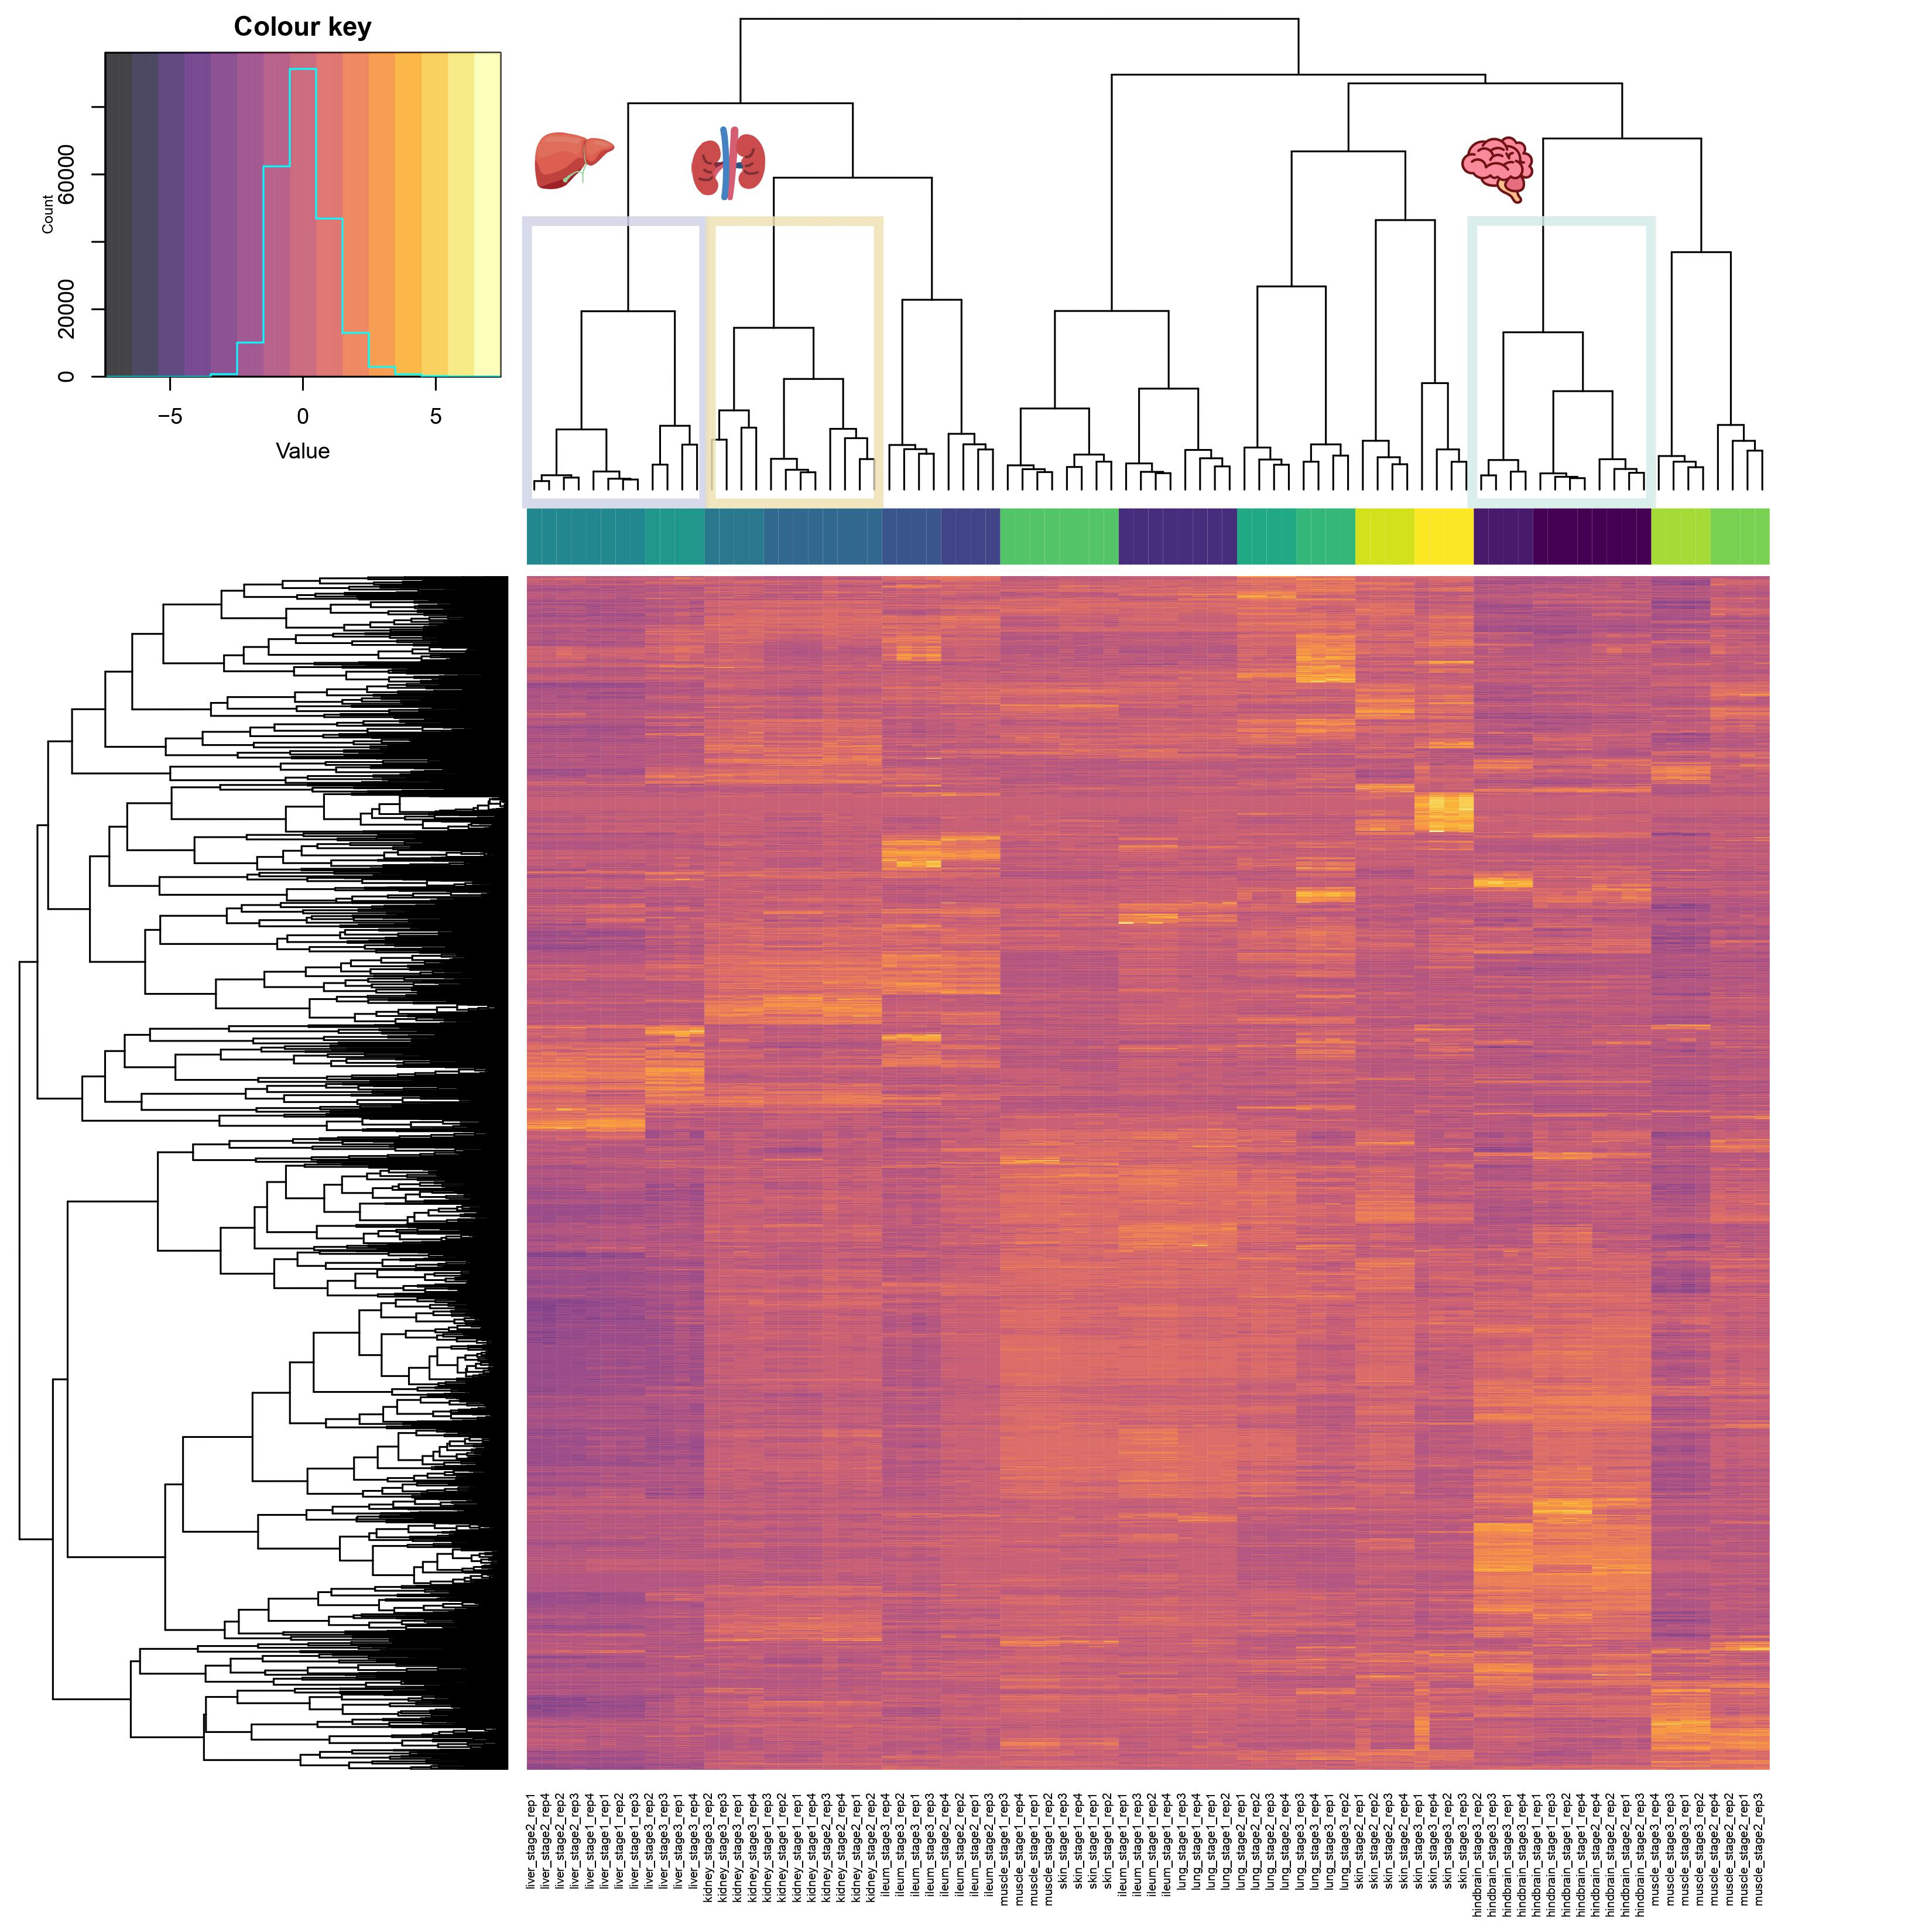
\includegraphics[width=\linewidth]{CLUSTERING.jpg}
    \caption{Hierarchical clustering results of TPM (Transcripts Per Million) 
	gene expression data of all samples. Genes are clustered in rows, and samples 
	are in columns. The row z-score corresponds to the fact that gene expression 
	data has been mean-centered and scaled, as $z = \frac{(y - \mu)}{sd}$. Stage 
	1 denotes 30 days post-fertilization, stage 2 denotes 70 days post-fertilization, 
	and stage 3 denotes newborn. There are four replicates for each tissue at 
	developmental stage.}
    \label{fig:hclust}
\end{figure*}
\clearpage

Moreover, we utilized the results from hierarchical clustering to decide where 
we should apply 
fusion penalties during regularization for network extraction, therefore 
informing the penalty matrices.
Liver, lung, kidney and hindbrain samples clustered by tissue, while
ileum, muscle and skin clustered 
by developmental stage. Additionally, the following
samples originaing from the same germ layer clustered more 
closely together, than with other samples: 

\begin{itemize}
    \item Liver 30dpf – Liver 70dpf
    \item Lung 30dpf – Ileum 30dpf
    \item Lung 70dpf – Lung NB
    \item Ileum 70dpf – Ileum NB
    \item Kidney 70dpf – Kidney NB
    \item Muscle 70dpf – Muscle NB
    \item Hindbrain 30dpf – Hindbrain 70dpf
    \item Skin 70dpf – Skin NB
\end{itemize}

\noindent This information has been reflected in the penalty matrices,
seprate for each embryological layer, as seen in the \nameref{netextr-meth}.

\subsection{\normalsize Network Extraction}\label{netextr}
Here we present the results from jointly estimating multiple regularized 
partial correlation matrices 
under optimal penalty matrices informed by the hierarchical clustering 
results. The optimal ridge and fusion 
penalty parameters estimated for each embryological layer are demonstrated.
The optimal penalties were determined by LOOCV for all genes present 
in germ layer-specific unions. 
The optimal penalties for the 61 genes found in all endoderm 
samples were

\[
\resizebox{\columnwidth}{!}{%
    $\bm{\varLambda}^{En} = 
    \begin{blockarray}{*{10}{c}}
     & \mathbf{L30} & \mathbf{L70} & \mathbf{LNB} & \mathbf{Lu30} & \mathbf{Lu70} & \mathbf{LuNB} & \mathbf{I30} & \mathbf{I70} & \mathbf{INB} \\
    \begin{block}{c [ccccccccc]}
    \mathbf{L30} & 2.34 \times 10^{2} & 5.16 \times 10^{-20} & 0 & 0 & 0 & 0 & 0 & 0 & 0 \\
    \mathbf{L70} & 5.16 \times 10^{-20} & 3.83 \times 10^{2} & 0 & 0 & 0 & 0 & 0 & 0 & 0 \\
    \mathbf{LNB} & 0 & 0 & 2.37 \times 10^{11} & 0 & 0 & 0 & 0 & 0 & 0 \\
    \mathbf{Lu30} & 0 & 0 & 0 & 2.37 \times 10^{8} & 0 & 0 & 1.68 \times 10^{-21} & 0 & 0 \\
    \mathbf{Lu70} & 0 & 0 & 0 & 0 & 1.40 \times 10^{2} & 8.54 \times 10^{-17} & 0 & 0 & 0 \\
    \mathbf{LuNB} & 0 & 0 & 0 & 0 & 8.54 \times 10^{-17} & 2.39 & 0 & 0 & 0 \\
    \mathbf{I30} & 0 & 0 & 0 & 1.68 \times 10^{-21} & 0 & 0 & 9.16 \times 10^{2} & 0 & 0 \\
    \mathbf{I70} & 0 & 0 & 0 & 0 & 0 & 0 & 0 & 1.13 \times 10^{7} & 3.21 \times 10^{-25} \\
    \mathbf{INB} & 0 & 0 & 0 & 0 & 0 & 0 & 0 & 3.21 \times 10^{-25} & 6.91 \times 10^{2} \\
    \end{block}
    \end{blockarray}$},
\]

\noindent for 48 genes present in all mesoderm samples:

\[
\resizebox{0.9\columnwidth}{!}{
	$\bm{\varLambda}^{Me} = 
    \begin{blockarray}{l*{6}{c}}
     & \mathbf{K30} & \mathbf{K70} & \mathbf{KNB} & \mathbf{M30} & \mathbf{M70} & \mathbf{MNB} \\
    \begin{block}{l[cccccc]}
    \mathbf{K30} & 2.56 & 6.95 \times 10^{-23} & 0 & 0 & 0 & 0 \\
    \mathbf{K70} & 6.95 \times 10^{-23} & 2.17 \times 10^{6} & 0 & 0 & 0 & 0 \\
    \mathbf{KNB} & 0 & 0 & 2.08 \times 10^{2} & 0 & 0 & 0 \\
    \mathbf{M30} & 0 & 0 & 0 & 2.56 \times 10^{2} & 0 & 0 \\
    \mathbf{M70} & 0 & 0 & 0 & 0 & 2.28 \times 10^{2} & 1.83 \times 10^{-20} \\
    \mathbf{MNB} & 0 & 0 & 0 & 0 & 1.83 \times 10^{-20} & 2.42 \times 10^{7} \\
    \end{block}
    \end{blockarray}$},
\]

\noindent and 74 genes present in all ectoderm samples:

\[
\resizebox{0.9\columnwidth}{!}{
	$\bm{\varLambda}^{Ec} = 
    \begin{blockarray}{l*{6}{c}}
     & \mathbf{H30} & \mathbf{H70} & \mathbf{HNB} & \mathbf{S30} & \mathbf{S70} & \mathbf{SNB} \\
    \begin{block}{l[cccccc]}
    \mathbf{H30} & 2.07 \times 10^{2} & 1.23 \times 10^{-19} & 0 & 0 & 0 & 0 \\
    \mathbf{H70} & 1.23 \times 10^{-19} & 6.21 \times 10^9 & 0 & 0 & 0 & 0 \\
    \mathbf{HNB} & 0 & 0 & 3.49 \times 10^{7} & 0 & 0 & 0 \\
    \mathbf{S30} & 0 & 0 & 0 & 1.42 \times 10^{7} & 0 & 0 \\
    \mathbf{S70} & 0 & 0 & 0 & 0 & 6.86 \times 10^{2} & 2.69 \times 10^{-22} \\
    \mathbf{SNB} & 0 & 0 & 0 & 0 & 2.69 \times 10^{-22} & 1.18 \times 10^{2} \\
    \end{block}
    \end{blockarray}$}.
\]

\noindent The penalty values for every germ layer-specific network extraction 
indicated strong differences in class-specific partial correlation matrices, 
favoring 
class-specific regularization 
(class-specific ridge) over retaining entry-wise similarities between 
data classes (pair-specific fusion). 
Moreover,  we used spectral condition 
number plots  to assess the conditioning of class-specific partial 
correlation matrices estimated under 
the optimal ridge penalties – an example plot can be found 
in Supplement (Figure \ref{fig:cnplot}).

\subsection{\normalsize Network Visualization}\label{netviz}
Following the optimal penalties extraction, conditioning assessment and 
support determination with a lFDR threshold of 0.99, we visualized the differential
networks. The following networks were empty:
\begin{itemize}
    \item Liver NB
    \item Lung 30dpf
    \item Intestine 70dpf
    \item Kidney 70dpf
    \item Hindbrain 70dpf
    \item Hindbrain NB
    \item Skin 30dpf
\end{itemize}
\noindent and therefore the differential visualizations could not be obtained for these 
tissues at developmental stages. We present the obtained differential networks in \nameref{diff-networks}.
Here, in Figure \ref{fig:liv30-70}, we provide an example of network obtained for liver between early organogenesis 
and late organogenesis.
\clearpage
\begin{figure*}[ht] % Two column figure (notice the starred environment)
    \centering
    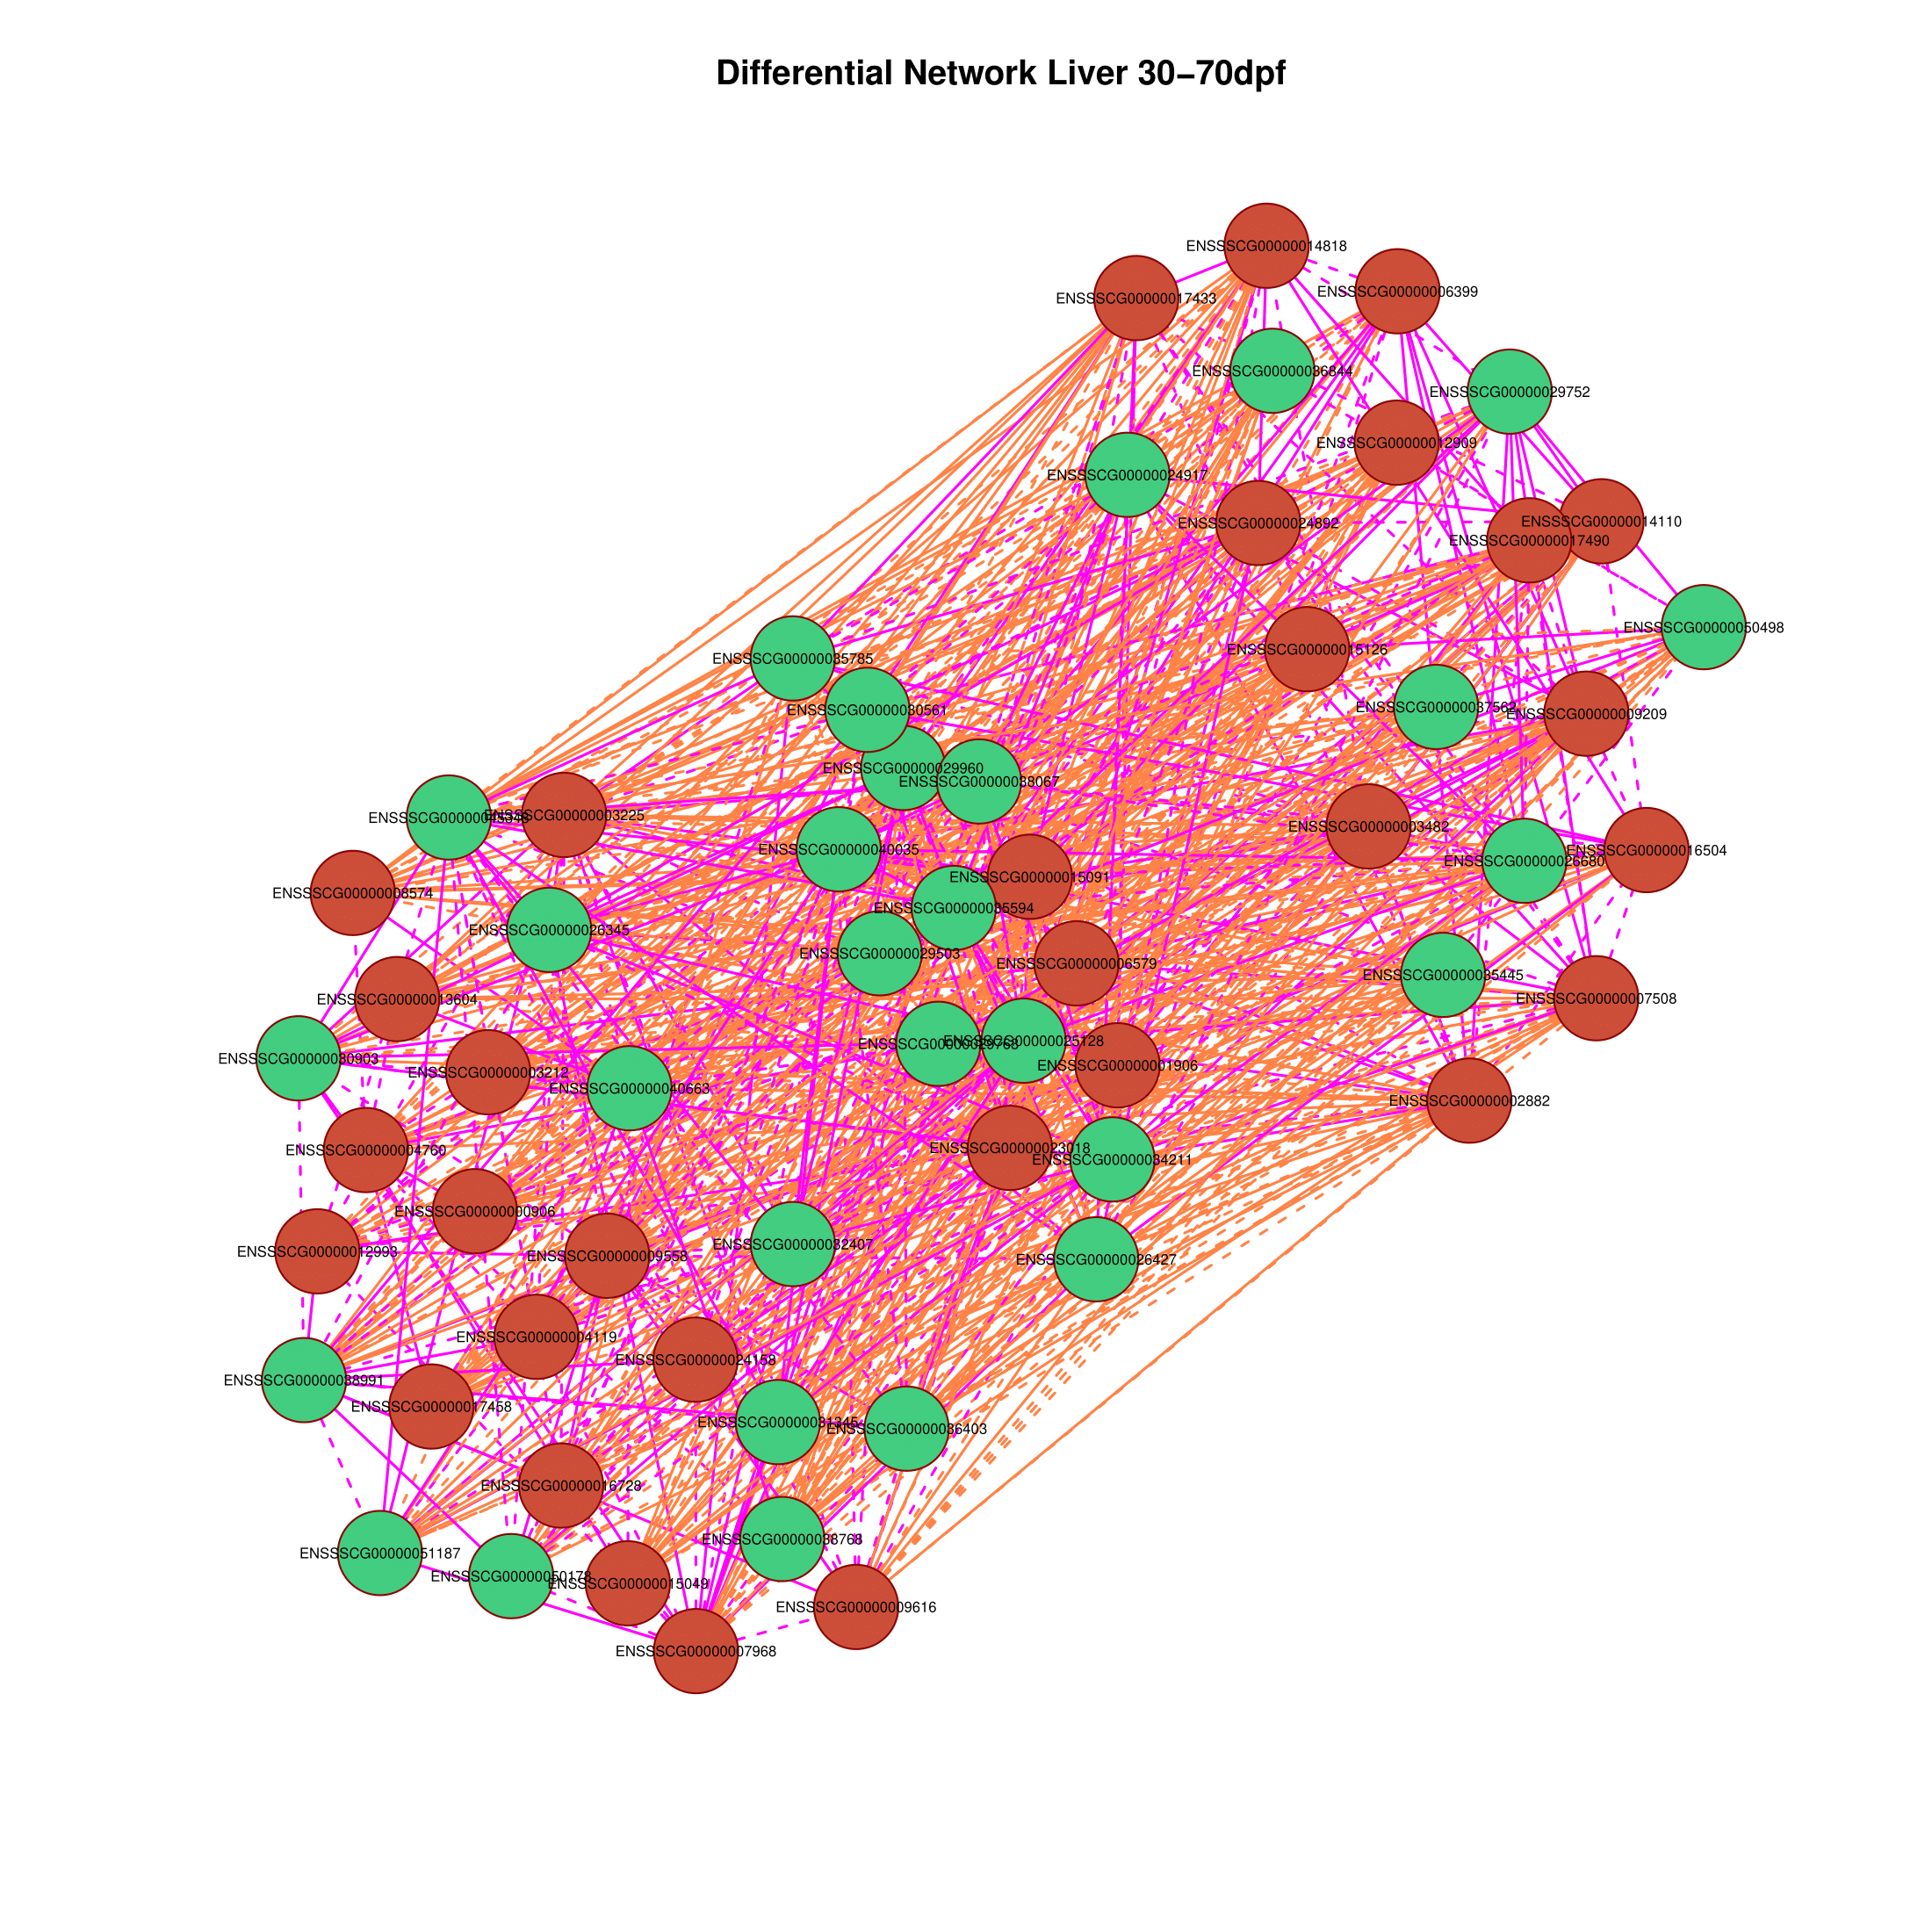
\includegraphics[width=\linewidth]{liver_30-70.png} % Adjust the width as needed
    \caption{Differential network between liver stage 30dpf and liver stage 70dpf. 
	Red nodes indicate up-regulated genes and green down-regulated genes. 
	Edges unique to class liver 30dpf are visualised in pink, while edges 
	unique to class liver 70dpf are in orange. Solid edges correspond to 
	positive partial correlations, whereas dashed edges indicate negatively 
	weighted partial correlations.}
	\label{fig:liv30-70}
\end{figure*}
\clearpage
In Lung 30-70dpf network three distinct edge clusters could be observed, whereas 
Lung 70dpf-NB, Muscle 70dpf-NB and Skin 70dpf-NB networks showed more of a \textit{hairball} 
structure. Moreover, Liver 30-70dpf and Skin 70dpf-NB were more densely connected than other differential networks extracted.
Furthermore, both in skin and muscle networks there were noticebaly more edges unique to class 70dpf,
while in lung network edges unique to class NB. Based on the networks' topology, we decided to determine
3 communities for each tissue-developmental stage combination. Networks viusalizing fluid community structure
can be found in \nameref{comm-det} sections of the Supplement (have to add more here). Following differential network visualizations
and community detection, we focused on analyzing the obtained networks.

\subsection{\normalsize Network Analysis}\label{netanal}
In this section we provide visual representations of gene set enrichment analysis with Enrichr using DESCARTES, 
whereas tables with more detailed results can be found in \nameref{net-anal} section of the Supplement. 
Additionally, we present results of TF overrepresentation analysis with ChEA3. We give our findings
per tissue at developmental stage.

\subsection{\small Endoderm}
Starting with liver 30dpf, the betweenness centrality of genes extracted for  
downstream analyses was between 3.45 and 33.50. 
Two cell types showed significant enrichment after 
adjusting the p-value using the Benjamini-Hochberg method, namely \textit{Ductal Cells in Pacreas}
and \textit{Lymphoid Cells in Liver}, as seen in Figure 1.

\begin{figure}[H] % Single column figure
	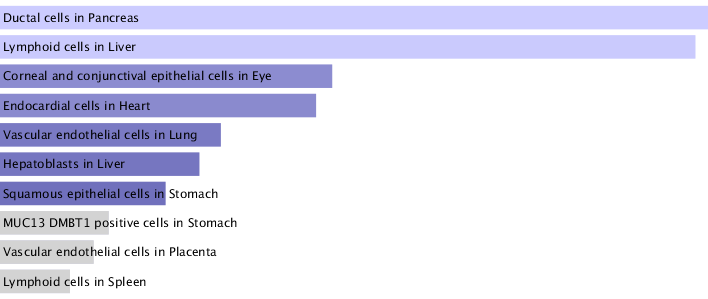
\includegraphics[width=\linewidth]{liver30_enrichment.png}
	\caption{Bar graph representing Enrichr gene set enrichment analysis results for 18 genes
	with the highest betweenness centrality in the liver 30dpf network. Enrichment 
	was conducted using Descartes Cell Types and Tissue 2021. Longer and lighter
	bars indicate more significant results. The results are sorted on
	the p-value. Gray colored bars indicate that terms 
	have not passed statistical significance (p-value).}
	\label{fig:liv30enr}
\end{figure}

\noindent The enrichment for \textit{Ductal Cells in Pancreas} is not suprising, as
the endocrine, exocrine and ductal components of the pancreas originate from endoderm \autocite{mccracken2012a}. 
Furthermore, fetal liver has been recognized as the major site of the development of 
the immune system, supporting the enrichment for \textit{Lymhoid Cells in Liver} in 
a list of high betweennes centrality genes from the liver 30dpf network \autocite{gale1987a}. Additionally,
the innate immune lympoid cells can also travel to other sites of organogenesis in the developing
fetus through blood \autocite{miller2018a}. Moving to the TFs, we identified KCNIP3, CREB3L3,
MRFL, BARX2 and GRHL3 to be the most substantially overepresented for liver 30dpf (see Table 4). 

\begin{table}[H]
	\caption{Transcription Factor Target Over-representation Analysis results for 18 genes with the highest betweenness centrality in the liver 30dpf network from the ChEA3 web tool.}
	\label{tab:liver30_tf}
	\resizebox{\columnwidth}{!}{%
	\begin{tabular}{ccccc}
	\hline
	\rowcolor[HTML]{FFFFFF} 
	\textbf{Rank} & \textbf{TF} & \textbf{Mean Rank} & \textbf{Overlapping Genes} & \textbf{Gene IDs} \\ \hline
	\cellcolor[HTML]{FFFFFF}1 & {\color[HTML]{343434} KCNIP3} & \cellcolor[HTML]{FFFFFF}16.5 & \cellcolor[HTML]{FFFFFF}{\color[HTML]{000000} 2} & \cellcolor[HTML]{FFFFFF}LMTK3, LRRC4B \\
	\rowcolor[HTML]{FFFFFF} 
	2 & {\color[HTML]{000000} CREB3L3} & 33.67 & {\color[HTML]{000000} 5} & F7, SMIM24, RORC, CYP1A1, CPN2 \\
	\rowcolor[HTML]{FFFFFF} 
	3 & {\color[HTML]{000000} MRFL} & 45.0 & {\color[HTML]{000000} 2} & SMIM24, MUC2 \\
	\rowcolor[HTML]{FFFFFF} 
	4 & {\color[HTML]{000000} BARX2} & 50.0 & {\color[HTML]{000000} 3} & TRIM29, PRSS22, MPZL2 \\
	\rowcolor[HTML]{FFFFFF} 
	5 & {\color[HTML]{000000} GRHL3} & 52.33 & {\color[HTML]{000000} 3} & TRIM29, PRSS22, MPZL2 \\ \hline
	\end{tabular}%
	}
	\end{table}

\noindent cAMP responsive element-binding protein 3 like 3 (CREB3L3) is known to be 
primarily expressed in the liver and small intestine, cooperating to 
maintain lipid matabolism \autocite{nakagawa2021a}. Furthermore, BarH-like homeobox 2 (BARX2)
is crucial during embryonic development, being involved in the epithelial-mesenchymal 
interactions of organogenesis, and cytoskeletal organization \autocite{ma2020a, naka2009a}. 
The expression of BARX2 is downregulated by CpG Island hypermethylation \autocite{ma2020a}.

Continuing with the next developmental stage, the betweenness centrality of liver genes extracted for  
downstream analyses was between 24.35 and 28.71. 
As vizualized in Figure 2, the following cell types showed significant enrcihment after FDR correction: \textit{Lymphoid cells in Heart},
\textit{Lymphoid cells in Lung}, \textit{Lymphoid cells in Pancreas}, 
\textit{Lymphoid cells in Intestine} and \textit{Lymphoid cells in Adrenal}.

\begin{figure}[H] % Single column figure
	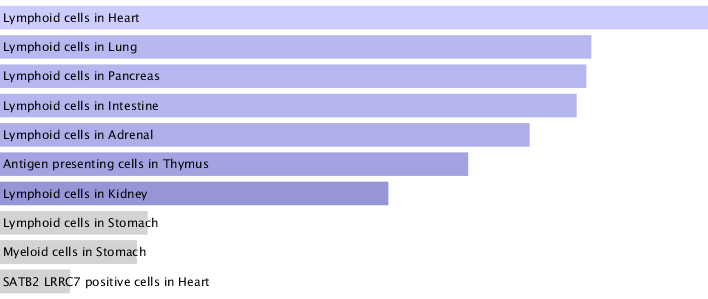
\includegraphics[width=\linewidth]{liver70_enrichment.png}
	\caption{Enrichr gene set enrichment analysis results for 17 genes
	with the highest betweenness centrality in the liver 70dpf network. Enrichment 
	was conducted using Descartes Cell Types and Tissue 2021.Longer and lighter
	bars indicate more significant results. The results are sorted on
	the p-value. Gray colored bars indicate that terms 
	have not passed statistical significance (p-value).}
	\label{fig:liv70enr}
\end{figure}

\noindent Altough the adrenal medulla originates from mesoderm, while the adrenal
cortex from ectoderm, we already established that the innate immune lympoid cells
can travel between organogenesis sites \autocite{gale1987a, nicolaides2000a, farraj2023a}. 
Moreover, the fetal liver has been 
shown to accomodate progenitors of various types of lymphoid cells \autocite{gale1987a}.
Next, we identified IRPF9, ZNF831, BATF2,
SCML4 and TBX21 to be the most substantially ovverepresented TFs for liver 70dpf (see Table 5).

\begin{table}[H]
	\caption{Transcription Factor Target Over-representation Analysis results for 17 genes with the highest betweenness centrality in the liver 70dpf network from the ChEA3 web tool.}
	\label{tab:liv70_tf}
	\resizebox{\columnwidth}{!}{%
	\begin{tabular}{
	>{\columncolor[HTML]{FFFFFF}}c 
	>{\columncolor[HTML]{FFFFFF}}c 
	>{\columncolor[HTML]{FFFFFF}}c 
	>{\columncolor[HTML]{FFFFFF}}c 
	>{\columncolor[HTML]{FFFFFF}}c }
	\hline
	\textbf{Rank} & \textbf{TF} & \textbf{Mean Rank} & \textbf{Overlapping Genes} & \textbf{Gene IDs} \\ \hline
	1 & {\color[HTML]{000000} IRF9} & 14.75 & {\color[HTML]{000000} 7} & NAPSA, IFI35, PTPRCAP, GPR37L1, SLC2A4RG, MYO1F, HERPUD1 \\
	2 & {\color[HTML]{000000} ZNF831} & 16.33 & {\color[HTML]{000000} 3} & GPR171, PTPRCAP, MYO1F \\
	3 & {\color[HTML]{000000} BATF2} & 27.33 & {\color[HTML]{000000} 3} & NAPSA, IFI35, MYO1F \\
	4 & {\color[HTML]{000000} SCML4} & 28.33 & {\color[HTML]{000000} 3} & GPR171, PTPRCAP, MYO1F \\
	5 & {\color[HTML]{000000} TBX21} & 29.25 & {\color[HTML]{000000} 5} & NAPSA, GPR171, PTPRCAP, MYO1F, HERPUD1 \\ \hline
	\end{tabular}%
	}
	\end{table}

\noindent Interferon regulatory factor 9 (IRF9) belongs to the IRF TF family involved in the 
transcriptional regulation of the immune system and cell growth, working
at the intersection of innate and adaptive immunity \autocite{paul2018a}.
Moreover, Basic leucine zipper ATF-like transcription factor 2 (BATF2) has been 
found to be a key factor in myeloid differentiation, therefore regulating
the immune response \autocite{le2023a}.

Moving on to the lung networks, the betweenness centrality of the 19 genes from the lung 70dpf 
network was between 3.26 and 3.51.	We identified no significantly enriched cell types after 
adjusting the p-value using the Benjamini-Hochberg method (Figure 3).
\begin{figure}[H] % Single column figure
	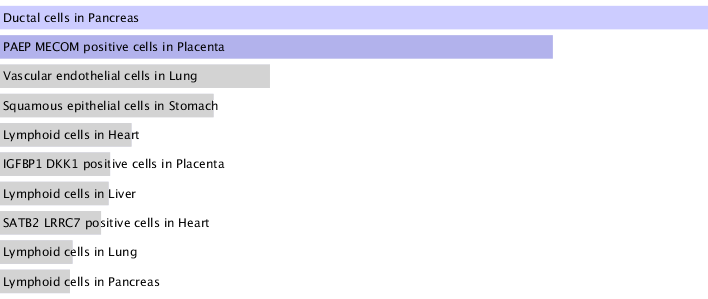
\includegraphics[width=\linewidth]{lung70_enrichment.png}
	\caption{Enrichr gene set enrichment analysis results for 19 genes
	with the highest betweenness centrality in the lung 70dpf network. Enrichment 
	was conducted using Descartes Cell Types and Tissue 2021. Longer and lighter
	bars indicate more significant results. The results are sorted on
	the p-value. Gray colored bars indicate that terms have
	not passed statistical significance (p-value).}
	\label{fig:lung70enr}
\end{figure}

\noindent However, without the correction, similarly to liver 70dpf, in 
lung 70dpf network \textit{Ductal cells in Pancreas}
were the most enriched term. The second most significant term was
\textit{PAEP MECOM positive cells in Placenta} (p-value = 0.01232). 
In male human fetus both \textit{PAEP}-positive and \textit{MECOM}-positive
cells in placenta were associated with the expression of \textit{Xist} 
or \textit{Tsix} gene \autocite{cao2020a}. \textit{Xist} encodes a long non-coding RNA (lncRNA)
that coats one of the X chromosomes in females, leading X chromosome inactivation 
to achieve dosage compensation between genders \autocite{cerase2015a}. \textit{Tsix} is a lncRNA
antisense to \textit{Xist} \autocite{lee1999a}. The presence of these markers is of maternal origin and while
\textit{Xist} corresponds to maternal decidualized stromal cells,
\textit{Tsix} corresponds to maternal endometrial epithelial cells \autocite{cao2020a}.
Next, we identified FOXN1, RBPJL, NR1D1, TBPL2 and CENPB
to be the most substantially ovverepresented TFs for lung 70dpf (see Table 6). 

\begin{table}[H]
	\caption{Transcription Factor Target Over-representation Analysis results for 19 genes with the highest betweenness centrality in the lung 70dpf network from the ChEA3 web tool.}
	\label{tab:lung70_tf}
	\resizebox{\columnwidth}{!}{%
	\begin{tabular}{
	>{\columncolor[HTML]{FFFFFF}}c 
	>{\columncolor[HTML]{FFFFFF}}c 
	>{\columncolor[HTML]{FFFFFF}}c 
	>{\columncolor[HTML]{FFFFFF}}c 
	>{\columncolor[HTML]{FFFFFF}}c }
	\hline
	\textbf{Rank} & \textbf{TF} & \textbf{Mean Rank} & \textbf{Overlapping Genes} & \textbf{Gene IDs} \\ \hline
	1 & {\color[HTML]{000000} FOXN1} & 31.67 & {\color[HTML]{000000} 4} & KRTDAP, CDSN, S100A3, VSIG8 \\
	2 & {\color[HTML]{000000} RBPJL} & 33.33 & {\color[HTML]{000000} 4} & RORC, SLC25A45, PRSS22, HERPUD1 \\
	3 & {\color[HTML]{000000} NR1D1} & 49.33 & {\color[HTML]{000000} 5} & KRTDAP, NAPSA, CDSN, PRSS22, HERPUD1 \\
	4 & {\color[HTML]{000000} TBPL2} & 51.5 & {\color[HTML]{000000} 4} & KRTDAP, NAPSA, CDSN, PRSS22, HERPA45 \\
	5 & {\color[HTML]{000000} CENPB} & 70.67 & {\color[HTML]{000000} 3} & NAPSA, GPR37L1, SLC2A4RG \\ \hline
	\end{tabular}%
	}
	\end{table}

\noindent 

\noindent Forkhead box protein N1 (FOXN1) is responsible for 
thymus organogenesis, by regulating thymic epithelial cells (TECs), therefore
contributing to in utero T-cell development, and aiding the immune response \autocite{vigliano2011a, reis2015a, moses2023a}.

Conversely, the betweennes centrality of 26 genes extracted from lung NB
network was equal to 1.67, the lowest from all tissues at developmental stages. 
After FDR correction no terms showed significant enrichment. The cell types with the highest
p-value were \textit{Ductal cells in Pancreas} (0.01056), similar to 
liver 30dpf and lung 70dpf, and 
\textit{IGFBP1 DKK1 positive cells in Placenta} (0.01107), as shown in Figure 4.

\begin{figure}[H] % Single column figure
	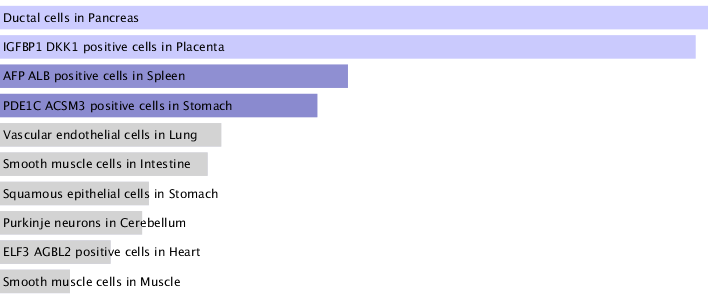
\includegraphics[width=\linewidth]{lungNB_enrichment.png}
	\caption{Enrichr gene set enrichment analysis results for 26 genes
	with the highest betweenness centrality in the lung NB network. Enrichment 
	was conducted using Descartes Cell Types and Tissue 2021.Longer and lighter
	bars indicate more significant results. The results are sorted on
	the adjusted p-value. Gray colored bars indicate that terms have 
	not passed statistical significance (p-value).}
	\label{fig:lungNBenr}
\end{figure}

\noindent Insulin-like growth factor-binding protein 1 (IGFBP1), 
and Dickkopf-related protein 1 (DKK1) are marker genes associated with decidual cells, 
which the decidua (pregnant endometrium) 
consists of, while the immune cells are one of the main cell types making up 
the decidual cells \autocite{wang2022a, farine2018a}. Subsequently, we identified OSR1, NR1I3, BATF2, IRF9, and IRF7 
to be the most ovverepresented TFs for lung NB (see Table 7).

\begin{table}[H]
	\caption{Transcription Factor Target Over-representation Analysis results for 26 genes with the highest betweenness centrality in the lung NB network from the ChEA3 web tool.}
	\label{tab:lungNB_tf}
	\resizebox{\columnwidth}{!}{%
	\begin{tabular}{
	>{\columncolor[HTML]{FFFFFF}}c 
	>{\columncolor[HTML]{FFFFFF}}c 
	>{\columncolor[HTML]{FFFFFF}}c 
	>{\columncolor[HTML]{FFFFFF}}c 
	>{\columncolor[HTML]{FFFFFF}}c }
	\hline
	\textbf{Rank} & \textbf{TF} & \textbf{Mean Rank} & \textbf{Overlapping Genes} & \textbf{Gene IDs} \\ \hline
	1 & {\color[HTML]{000000} OSR1} & 26.0 & {\color[HTML]{000000} 3} & RHBDF1, ANO1, FAM180A \\
	2 & {\color[HTML]{000000} NR1I3} & 29.33 & {\color[HTML]{000000} 5} & DMGDH, IGFBP1, F7, CYP1A1, SLC25A45 \\
	3 & {\color[HTML]{000000} BATF2} & 34.0 & {\color[HTML]{000000} 3} & ZBP1, NAPSA, IFI35 \\
	4 & {\color[HTML]{000000} IRF9} & 50.0 & {\color[HTML]{000000} 5} & ZBP1, NAPSA, IFI35, GPR37L1, SLC25A45 \\
	5 & {\color[HTML]{000000} IRF7} & 54.33 & {\color[HTML]{000000} 2} & ZBP1, IFI35 \\ \hline
	\end{tabular}%
	}
	\end{table}

\noindent Odd skipped-related 1 (OSR1) is associated with connective tissue formation
and myogenesis in limbs, pointing towards mesoderm development, whereas 
\textit{constitutive androstane receptor} (NR1I3) expression is enriched in adult mammalian liver
and its expression in human embryonic stem cells has been linked to 
differentiation and maturation of hepatic-like cells \autocite{vallecillogarc2017a, chen2013b}.

\subsection{\small Mesoderm}
Continuing with mesoderm networks, the betweenness centrality of  24 genes 
from the muscle 70dpf network was between 2.55 and 3.07. We didn't find any statistically
significant terms after FDR correction. The top two enriched cell types were 
\textit{Megakaryocytes in Lung} and \textit{Megakaryocytes in Muscle} (Figure 5).

\begin{figure}[H] % Single column figure
	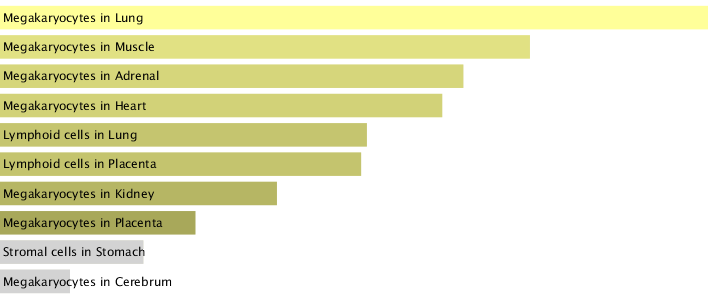
\includegraphics[width=\linewidth]{muscle70_enrichment.png}
	\caption{Enrichr gene set enrichment analysis results for 24 genes
	with the highest betweenness centrality in the muscle 70dpf network. Enrichment 
	was conducted using Descartes Cell Types and Tissue 2021. Longer and lighter
	bars indicate more significant results. The results are sorted on
	the p-value. Gray colored bars indicate that terms have 
	not passed statistical significance (p-value).}
	\label{fig:muscle70enr}
\end{figure}

\noindent Megakaryotes are rare cells found in the bone marrow, reponsible for the
production of platelets, which aid the formation of blod clots
and wound healing \autocite{davenport2022a}. Apart from assisting thrombosis,
platelets are know to influence the immune response as well, by e.g., directing T-cell
activation and differentiation \autocite{ali2015a, koupenova2022a}.
Moeover, platelet-producing megakaryotes residing in the lung have
been shown to have key immune regulatory roles \autocite{pariser2021a}.

\noindent Eventually, we looked into top enriched TFs for genes with
high betweenness centrality in muscle 70dpf network. In Table 8 we present
the results from this enrichment analysis.

\begin{table}[H]
	\caption{Transcription Factor Target Over-representation Analysis results for 24 genes with the highest betweenness centrality in the muscle 70dpf network from the ChEA3 web tool.}
	\label{tab:muscle70_tf}
	\resizebox{\columnwidth}{!}{%
	\begin{tabular}{
	>{\columncolor[HTML]{FFFFFF}}c 
	>{\columncolor[HTML]{FFFFFF}}c 
	>{\columncolor[HTML]{FFFFFF}}c 
	>{\columncolor[HTML]{FFFFFF}}c 
	>{\columncolor[HTML]{FFFFFF}}c }
	\hline
	\textbf{Rank} & \textbf{TF} & \textbf{Mean Rank} & \textbf{Overlapping Genes} & \textbf{Gene IDs} \\ \hline
	1 & {\color[HTML]{000000} SP140L} & 13.0 & {\color[HTML]{000000} 4} & MAP4K1, ZBP1, SCML4, UNC13D \\
	2 & {\color[HTML]{000000} ZNF831} & 24.0 & {\color[HTML]{000000} 5} & MAP4K1, ZBP1, SCML4, MSLNL, UNC13D \\
	3 & {\color[HTML]{000000} SP110} & 40.67 & {\color[HTML]{000000} 5} & ZBP1, MAP4K1, SCML4, TREML2, UNC13D \\
	4 & {\color[HTML]{000000} THRA} & 48.25 & {\color[HTML]{000000} 8} & ZBP1, TEF, NFIC, MLC1, SH2B2, NRGN, SPTBN2, RIBC2 \\
	5 & {\color[HTML]{000000} SCX} & 49.0 & {\color[HTML]{000000} 2} & NFIC, MDFI \\ \hline
	\end{tabular}%
	}
	\end{table}

\noindent The top enriched TFs for muscle 70dpf were SP140L, ZNF831, SP110,
THRA, and SCX. The speckled protein (SP) family members are primarily 
expressed in leukocytes, and the 
SP140 locus has been associated with multiple autoimmune diseases, such
as multiple sclerosis (MS), which is considered to be 
a T-cell-mediated disease \autocite{karaky2018a}. Furthermore, zinc finder protein 831 (ZNF831), 
that was enriched in liver 70dpf as well, is a tumour supressor
linked to immune activity and apoptosis in breast cancer \autocite{fan2022a}.

Continuing with muscle NB genes. The betweenness centrality of
the 11 genes extracted for downstream analyses was between 22.45 and 35.17.
After applying FRD correction, there were no significantly enriched terms.
The top cell types as seen in Figure 6
were \textit{Vascular endothelial cells in Stomach} and 
\textit{Smooth muscle cells in Heart}.

\begin{figure}[H] % Single column figure
	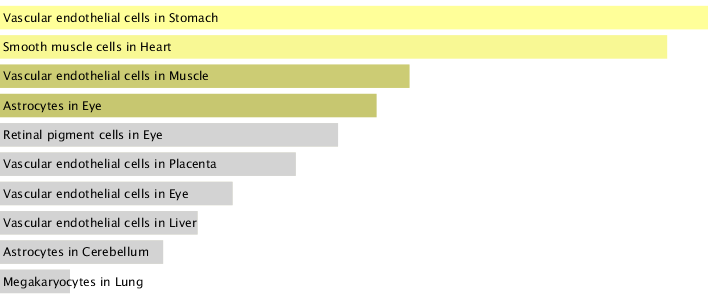
\includegraphics[width=\linewidth]{muscleNB_enrichment.png}
	\caption{Enrichr gene set enrichment analysis results for 11 genes
	with the highest betweenness centrality in the muscle NB network. Enrichment 
	was conducted using Descartes Cell Types and Tissue 2021. Longer and lighter
	bars indicate more significant results. The results are sorted on
	the p-value. Gray colored bars indicate that terms have 
	not passed statistical significance (p-value).}
	\label{fig:muscleNBenr}
\end{figure}

\noindent The vascular endothelium, consisting of endothelial cells (EC) forming a single layer,
lines the interior of arteries, veins, and capillaries, facilitating develment and maintenance
of the circulatory system. The endothelium functions as an endocrine, i.e., hormonal 
organ as well \autocite{kruegergenge2019a, trimm2023a}. Both cardiovascular system and musculoskeletal system
originate from the mesoderm \autocite{ferretti2019a}. Focusing on TF overrepresentation analysis,
the top five overrepresented TFs for muscle NB were OLIG1, MEOX1, DBX2, SOX18, and POUF3F2 (see Table 9).

\begin{table}[H]
	\caption{Transcription Factor Target Over-representation Analysis results for 10 genes with the highest betweenness centrality in the muscle NB network from the ChEA3 web tool.}
	\label{tab:muscleNB_tf}
	\resizebox{\columnwidth}{!}{%
	\begin{tabular}{
	>{\columncolor[HTML]{FFFFFF}}c 
	>{\columncolor[HTML]{FFFFFF}}c 
	>{\columncolor[HTML]{FFFFFF}}c 
	>{\columncolor[HTML]{FFFFFF}}c 
	>{\columncolor[HTML]{FFFFFF}}c }
	\hline
	\textbf{Rank} & \textbf{TF} & \textbf{Mean Rank} & \textbf{Overlapping Genes} & \textbf{Gene IDs} \\ \hline
	1 & {\color[HTML]{000000} OLIG1} & 25.0 & {\color[HTML]{000000} 1} & MLC1 \\
	2 & {\color[HTML]{000000} MEOX1} & 39.67 & {\color[HTML]{000000} 2} & CCM2L, CYGB \\
	3 & {\color[HTML]{000000} DBX2} & 43.33 & {\color[HTML]{000000} 1} & MLC1 \\
	4 & {\color[HTML]{000000} SOX18} & 62.67 & {\color[HTML]{000000} 2} & CCM2L, CYGB \\
	5 & {\color[HTML]{000000} POUF3F2} & 68.0 & {\color[HTML]{000000} 2} & PEG10, MLC1 \\ \hline
	\end{tabular}%
	}
	\end{table}

\noindent Oligodendrocyte transcription factor 1 (OLIG1) is crucial for 
maturation of oligodendrocyte precursor cells contributing to the development
of central nervous system involving all three germ layers \autocite{zhao2019a, elshazzly2023a}.
Furthermore, mesenchyme homeobox 1 (MEOX1) has been identified
as a positive regulator of smooth muscle cell differentiation
during embryogenesis in mice \autocite{dong2018a}.

\subsection{\small Ectoderm}
Continuing with the 16 genes with the highest betweenness centrality in the skin 70dpf
(values between 6.40 and 6.52), we didn't get any significant cell type enrichment 
results (Figure 7).

\begin{figure}[H] % Single column figure
	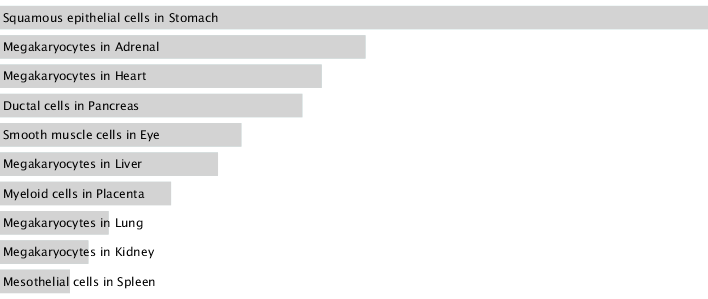
\includegraphics[width=\linewidth]{skin70_enrichment.png}
	\caption{Enrichr gene set enrichment analysis results for 16 genes
	with the highest betweenness centrality in the skin 70dpf network. Enrichment 
	was conducted using Descartes Cell Types and Tissue 2021. Longer and lighter
	bars indicate more significant results. The results are sorted on
	the adjusted p-value. Gray colored bars indicate that terms have 
	not passed statistical significance (p-value).}
	\label{fig:skin70enr}
\end{figure}

\noindent The top five overrepresented TFs we identified for skin 70dpf genes were
KCNIP3, EBF4, BATF2, SOX9, and ARID5A (Table 10).

\begin{table}[H]
	\caption{Transcription Factor Target Over-representation Analysis results for 10 genes with the highest betweenness centrality in the skin 70dpf network from the ChEA3 web tool.}
	\label{tab:skin70_tf}
	\resizebox{\columnwidth}{!}{%
	\begin{tabular}{
	>{\columncolor[HTML]{FFFFFF}}c 
	>{\columncolor[HTML]{FFFFFF}}c 
	>{\columncolor[HTML]{FFFFFF}}c 
	>{\columncolor[HTML]{FFFFFF}}c 
	>{\columncolor[HTML]{FFFFFF}}c }
	\hline
	\textbf{Rank} & \textbf{TF} & \textbf{Mean Rank} & \textbf{Overlapping Genes} & \textbf{Gene IDs} \\ \hline
	1 & {\color[HTML]{000000} KCNIP3} & 45.5 & {\color[HTML]{000000} 1} & NRGN \\
	2 & {\color[HTML]{000000} EBF4} & 58.0 & {\color[HTML]{000000} 3} & NTNG2, ADGRG1, TNRC18 \\
	3 & {\color[HTML]{000000} BATF2} & 77.0 & {\color[HTML]{000000} 2} & NTNG2, IFI35 \\
	4 & {\color[HTML]{000000} SOX9} & 77.2 & {\color[HTML]{000000} 3} & ADGRG1, TNRC18, NRGN \\
	5 & {\color[HTML]{000000} ARID5A} & 80.5 & {\color[HTML]{000000} 3} & SH3TC1, NR1H2, IFI35 \\ \hline
	\end{tabular}%
	}
	\end{table}

\noindent We have already introduced KCNIP3 in the liver 30dpf section, 
while BATF2 liver 70dpf and lung NB sections.
Furthermore, we found that Early B cell factor 4 (EBF4) is expressed in human immune
cells, playing a role cytotoxic lymphocyte function,
therefore aiding the immune response \autocite{kubo2022a}.

At last, we looked at 9 genes with the highest betweennes centrality
in the skin NB network. Although their values were high compared to 
other tissues at developmental stages (between 62 and 74.2), we identified
only one signficantly enriched cell type after FDR correction, namely
\textit{Megakaryocytes in Muscle} (Figure 8). We discussed
megakaryotes in the muscle 70dpf section.

\begin{figure}[H] % Single column figure
	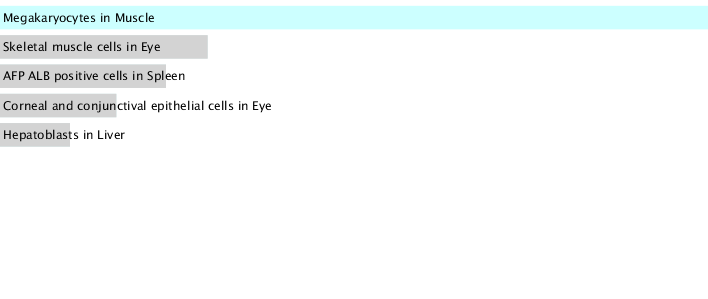
\includegraphics[width=\linewidth]{skinNB_enrichment.png}
	\caption{Enrichr gene set enrichment analysis results for 9 genes
	with the highest betweenness centrality in the skin NB network. Enrichment 
	was conducted using Descartes Cell Types and Tissue 2021. Longer and lighter
	bars indicate more significant results. The results are sorted on
	the p-value. Gray colored bars indicate that terms have 
	not passed statistical significance (p-value).}
	\label{fig:skinNBenr}
\end{figure}

\noindent Moreover, we looked at overrepresented TFs in skin NB networks, 
and identified ZNF605, ZNF154, ZNF221, ZNF780B, and ZNF626 (Table 11).

\begin{table}[H]
	\caption{Transcription Factor Target Over-representation Analysis results for 10 genes with the highest betweenness centrality in the skin NB network from the ChEA3 web tool.}
	\label{tab:skinNB_tf}
	\resizebox{\columnwidth}{!}{%
	\begin{tabular}{
	>{\columncolor[HTML]{FFFFFF}}c 
	>{\columncolor[HTML]{FFFFFF}}c 
	>{\columncolor[HTML]{FFFFFF}}c 
	>{\columncolor[HTML]{FFFFFF}}c 
	>{\columncolor[HTML]{FFFFFF}}c }
	\hline
	\textbf{Rank} & \textbf{TF} & \textbf{Mean Rank} & \textbf{Overlapping Genes} & \textbf{Gene IDs} \\ \hline
	1 & {\color[HTML]{000000} ZNF605} & 19.33 & {\color[HTML]{000000} 3} & ZNF37A, PEG10, PCBD2 \\
	2 & {\color[HTML]{000000} ZNF154} & 66.67 & {\color[HTML]{000000} 3} & ZNF37A, GPX7, PCBD2 \\
	3 & {\color[HTML]{000000} ZNF221} & 72.0 & {\color[HTML]{000000} 1} & ZNF37A \\
	4 & {\color[HTML]{000000} ZNF780B} & 93.0 & {\color[HTML]{000000} 1} & ZNF37A \\
	5 & {\color[HTML]{000000} ZNF626} & 98.67 & {\color[HTML]{000000} 3} & ZNF37A, PEG10, PCBD2 \\ \hline
	\end{tabular}%
	}
	\end{table}

\noindent Interestingly, all top five TFs belonged to the zinc finder proteins (ZNF) family,
which is the largest TF family in the human genome \autocite{jen2016a}. In humans ZNF605, ZNF154, ZNF780B, and
ZNF626 exhibit the highest expression in thyroid (with thyroid hormones modulating a variety
of immune cells), whereas ZNF221 in brain 
(originating from ectoderm) \autocite{elshazzly2023a, sayers2022a, jara2017a}.

%------------------------------------------------

\section{\large Discussion}

As the omics revolution picks up pace, the need for novel approaches to analyzing 
high-throughput biological data ever-increasing in complexity and size, which can 
conquer the curse of dimensionality, becomes evident. 
At the same time, model interpretability and
visually appealing analytical approaches
are desirable. Therefore, we aimed to 
determine whether the joint ridge fusion regularization procedure 
informed with the results from hierarchical clustering 
of RNA-Seq data
can ensure the extraction of the relevant data signal 
in network modelling of DNA methylation data coming 
from multiple swine tissues and developmental stages.

The findings concerning hierarchical clustering of RNA-Seq data of 
samples showed liver, lung, kidney and hindbrain samples clustering 
by tissue, while ileum, muscle and skin clustered by developmental
stage. We assume that the difference with findings obtained by the 
GENE-SWitCH (lung clustering by developmental stage)
arises from the fact that we worked with a subset of the gene expression data.
We focused on CpG methylated at promoter regions DEGs between developmental stages,
and additionally we 
excluded genes located at the X chromosome from the analysis,
whereas GENE-SWitCH included all genes in the analysis \autocite{acloque2022a}.
Additionally, at 30dpf we observed lung and ileum, which
originte from endoderm, clustering together,
suggesting that during early organogenesis 
they have not yet fully differentiated.

Subsequently, we informed the penalty structures
with results from hierarchical clustering, to 
estimate the optimal penalty matrices for all 
germ layers separately. Ideally, we would have specified one
common penalty structure for all tissues and developmental stages together;
however, only one gene was shared between all data classes.
In that sense, our analysis might be considered naive, since we've 
ignored interplay between tissues originating from
different germ layers. Nevertheless, we continued with our approach,
having in mind that "Essentially, all models are wrong, but some are
useful" \autocite{nr1987a}.
We observed favouring of class-specific regularisation (class-specific ridge) 
over retainment of entry-wise similarities between data classes (pair-specific fusion) 
in all germ-layer specific penalty structures. This suggests that all data 
classes (tissues at developmental stages) are quite distinct 
concerning methylation patterns, 
further emphasising the dynamic nature of the (epi)genome.

The highest class-specific ridge penalty was evaluated by LOOCV for 
liver NB, indicating that the
precision matrix approached the target matrix, 
suggesting negligible signal in the data.
We also observed high ridge penalties for lung 30dpf,
intestine 70dpf, hindbrain 70dpf, hindbrain NB, 
and skin 30dpf, explaining empty networks obtained
for the abovementioned tissues at developmental stages.
However, we also got an empty network for kidney
at 70dpf, which had a relatively low ridge
penalty compared to other disscussed data classes 
($\lambda_{gg} = 2.50$). This would suggest that there's
a negligible methylation signal in kidney 
development during late organogenesis, compared
to early organogenesis and newborn stage.
Notably, all partial correlation matrices estimated under 
the optimal penalty parameters determined for germ layer-specific 
network extraction were well-conditioned, as suggested by 
condition number plots. This illustrates that the $l_2$ 
regularization procedure implemented with \texttt{rags2ridges}
led to well-conditioned estimates of the partial correlation 
matrices for network visualization and downstream analyses. 

Continuing with cell type and TF overrepresentation analysis,
using gene sets with the highest betweenness centrality
from each data class specific network, 
we observed biologically feasible results for each tissue.
Concerning the recurring trend of immune-response associated
terms for all tissues; a fetus is considered vulnerable
to infections in utero \autocite{luculligan2020a}. However, the
maternal-fetal
immunological lansdcape involving, e.g., the placenta, lymphoid cells,
and megakaryotes, supports the developing fetus
in all stages of pregnancy \autocite{hussain2022a}. The results obtained
suggests that our analytical framework allowed for extraction of
biologically feasible data signal.

However, our results should be approached with caution due to the limitations 
of contemporary omics research and the methodological constraints of the project itself. 
The sample size is the major issue to consider when aiming to accurately estimate network parameters and, therefore, 
the network topology. As introduced before, omics data analyses often suffer from the curse 
of dimensionality – therefore, we implemented joint fused ridge estimation. Nevertheless, 
conquering singularity does not solve the issues of difficulty collecting pig tissue samples, 
especially at early developmental stages. The considerations for ethical animal 
experimentation call for the adoption of the 4Rs principles (Reduction, Refinement, Replacement and Responsibility) 
\autocite{kiani2022a}, which in essence, require the least amount of biological replicates feasible to be 
collected. Moreover, there is often not enough genetic material in a single sample (which resulted in 
pooling of samples at 30dpf) and the desired sample itself is hard to extract, i.e., at 30dpf 
due to sampling uncertainty samples intended to be
cerebellum were labelled as hindbrain. 

Furthermore, genes involved in early development are often less well annotated than genes expressed 
in mature tissues. Additionally, literature on swine development at genomics resolution is scarce,
therefore we conducted enrichment analyses on the human orthologs. Not only does enrichment 
analysis suffer from these incomplete annotations, but 
the insights obtained from network analysis might not represent early developmental stages 
in swine accurately,
since we reviewed literature focusing on human and mice development. 
These limitations highlight the importance and novelty of the efforts of projects such as GENE-SWitCH. 

Additionally, we believe that our analyses would benefit from utilizing (epi)genomics
data measured at single-cell resolution, therefore accounting for tissue heterogenity
allowing us to extract networks more accurately representing methylation 
patterns during pig fetal development.

%----------------------------------------------

\section{\large Conclusions}

%----------------------------------------------

\section{\large Availability of Data and Materials}

%----------------------------------------------

\section{\large List of Abbreviations}  
    \begin{description}[leftmargin=*, widest=FR Algorithm]
    
        \item[DNMT]
        DNA Methyltransferase
        
        \item[CpG]
        5'—C—phosphate—G—3'
        
        \item[TSS]
        Transcription Start Site
        
        \item[FAANG]
        Functional Annotation of Animal Genomes consortium

		\item[RNA-Seq]
		RNA Sequencing
        
        \item[RRBS]
        Reduced Representation Bisulfite Sequencing

		\item[PCR]
		Polymerase Chain Reaction

		\item[30dpf] 
		30 days post fertilization
		
		\item[70dpf] 
		70 days post fertilization
		
		\item[NB] 
		Newborn 
		
		\item[ChIP-Seq] 
		Chromatin Immunoprecipitation assays with Sequncing
		
		\item[H3K4me3] 
		Histone 3 Lysine 4 trimethylation

		\item[bp] 
		Base pair

		\item[DEG]
		Differentially Expressed Gene

		\item[GGM] 
		Gaussian Graphical Model

		\item[NPN]
		Nonparanormal

		\item[CDF]
		Culmulative Distribution Function
		
		\item[ECDF]
		Empirical Culmulative Distribution Function

		\item[TPM]
		Transcripts Per Million

		\item[AWS]
		Average Silhouette Width

		\item[MLE]
		Maximum Likelihood Estimation

		\item[LOOCV]
		Leave One Out Cross Validation

		\item[lFDR]
		Local False Discovery Rate

		\item[FR algorithm]
		Fruchterman-Reingold algorithm

		\item{DESCARTES}
		Developmental Single Cell Atlas of Gene RegulaTion and Expression

		\item{TF}
		Transcription Factor

		\item[ChEA3]
		ChIP-X Enrichment Analysis Version 3

		\item[CREB3L3]
		cAMP responsive element-binding protein 3 like 3

		\item[BARX2]
		BarH-like homeobox 2

		\item[IRF9]
		Interferon regulatory factor 9

		\item[BATF2]
		Basic leucine zipper ATF-like transcription factor 2

		\item[lncRNA]
		Long non-coding RNA

		\item[IGFBP1]
		Insulin-like growth factor-binding protein 1
		
		\item[DKK1] 
		Dickkopf-related protein 1

		\item[OSR1]
		Odd skipped-related 1

		\item[NR1I3]
		Constitutive androstane receptor

		\item[SP]
		Speckled protein

		\item[MS]
		Multiple sclerosis

		\item[ZNF831]
		Zinc finder protein 831
        
		\item[EC]
		Endothelial cells

		\item[OLIG1]
		Oligodendrocyte transcription factor 1

		\item[MEOX1]
		Mesenchyme homeobox 1

		\item[EBF4]
		Early B cell factor 4

		\item[ZNF]
		Zinc finder protein

		\item[4Rs]
		Reduction, Refinement, Replacement, Responsibility


	\end{description}

\section{\large Supplementary Materials}\label{supplement}

\onecolumn\clearpage\subsection{\normalsize Extracted genes}\label{exgenes}
\begin{table*}[!ht]
	\caption{An overview of all genes used for modelling endoderm-specific networks.}
	\label{tab:genes_endoderm}
	\begin{threeparttable}
	\resizebox{\textwidth}{!}{%
	\begin{tabular}{lllll}
	\hline
	\rowcolor[HTML]{EFEFEF} 
	\multicolumn{1}{c}{\cellcolor[HTML]{EFEFEF}\textbf{g\#}} & \multicolumn{1}{c}{\cellcolor[HTML]{EFEFEF}\textbf{initial\_alias}} & \multicolumn{1}{c}{\cellcolor[HTML]{EFEFEF}\textbf{ortholog\_name}} & \multicolumn{1}{c}{\cellcolor[HTML]{EFEFEF}\textbf{ortholog\_ensg}} & \multicolumn{1}{c}{\cellcolor[HTML]{EFEFEF}{\color[HTML]{000000} \textbf{description}}} \\ \hline
	\multicolumn{1}{l|}{1} & ENSSSCG00000000906 & TMCC3 & ENSG00000057704 & transmembrane and coiled-coil domain family 3 {[}Source:HGNC   Symbol;Acc:HGNC:29199{]} \\
	\multicolumn{1}{l|}{2} & ENSSSCG00000001906 & CYP1A1 & ENSG00000140465 & cytochrome P450 family 1 subfamily A member 1 {[}Source:HGNC   Symbol;Acc:HGNC:2595{]} \\
	\multicolumn{1}{l|}{3} & ENSSSCG00000002882 & KRTDAP & ENSG00000188508 & keratinocyte differentiation associated protein {[}Source:HGNC   Symbol;Acc:HGNC:16313{]} \\
	\multicolumn{1}{l|}{4} & ENSSSCG00000003212 & NAPSA & ENSG00000131400 & napsin A aspartic peptidase {[}Source:HGNC Symbol;Acc:HGNC:13395{]} \\
	\multicolumn{1}{l|}{5} & ENSSSCG00000003225 & CEACAM18 & ENSG00000213822 & CEA cell adhesion molecule 18 {[}Source:HGNC Symbol;Acc:HGNC:31949{]} \\
	\multicolumn{1}{l|}{6} & ENSSSCG00000003482 & PADI3 & ENSG00000142619 & peptidyl arginine deiminase 3 {[}Source:HGNC Symbol;Acc:HGNC:18337{]} \\
	\multicolumn{1}{l|}{7} & ENSSSCG00000004119 & GRM1 & ENSG00000152822 & glutamate metabotropic receptor 1 {[}Source:HGNC Symbol;Acc:HGNC:4593{]} \\
	\multicolumn{1}{l|}{8} & ENSSSCG00000004760 & PPP1R14D & ENSG00000166143 & protein phosphatase 1 regulatory inhibitor subunit 14D {[}Source:HGNC   Symbol;Acc:HGNC:14953{]} \\
	\multicolumn{1}{l|}{9} & ENSSSCG00000006399 & VSIG8 & ENSG00000243284 & V-set and immunoglobulin domain containing 8 {[}Source:HGNC   Symbol;Acc:HGNC:32063{]} \\
	\multicolumn{1}{l|}{10} & ENSSSCG00000006579 & S100A3 & ENSG00000188015 & S100 calcium binding protein A3 {[}Source:HGNC Symbol;Acc:HGNC:10493{]} \\
	\multicolumn{1}{l|}{11} & ENSSSCG00000007508 & ZBP1 & ENSG00000124256 & Z-DNA binding protein 1 {[}Source:HGNC Symbol;Acc:HGNC:16176{]} \\
	\multicolumn{1}{l|}{12} & ENSSSCG00000007968 & RHBDF1 & ENSG00000007384 & rhomboid 5 homolog 1 {[}Source:HGNC Symbol;Acc:HGNC:20561{]} \\
	\multicolumn{1}{l|}{13} & ENSSSCG00000008574 & KIF3C & ENSG00000084731 & kinesin family member 3C {[}Source:HGNC Symbol;Acc:HGNC:6321{]} \\
	\multicolumn{1}{l|}{14} & ENSSSCG00000009209 & N/A & N/A & N/A \\
	\multicolumn{1}{l|}{15} & ENSSSCG00000009558 & F10 & ENSG00000126218 & coagulation factor X {[}Source:HGNC Symbol;Acc:HGNC:3528{]} \\
	\multicolumn{1}{l|}{16} & ENSSSCG00000009616 & HR & ENSG00000168453 & HR lysine demethylase and nuclear receptor corepressor {[}Source:HGNC   Symbol;Acc:HGNC:5172{]} \\
	\multicolumn{1}{l|}{17} & ENSSSCG00000012909 & PTPRCAP & ENSG00000213402 & protein tyrosine phosphatase receptor type C associated protein   {[}Source:HGNC Symbol;Acc:HGNC:9667{]} \\
	\multicolumn{1}{l|}{18} & ENSSSCG00000012993 & SLC25A45 & ENSG00000162241 & solute carrier family 25 member 45 {[}Source:HGNC Symbol;Acc:HGNC:27442{]} \\
	\multicolumn{1}{l|}{19} & ENSSSCG00000013604 & MYO1F & ENSG00000142347 & myosin IF {[}Source:HGNC Symbol;Acc:HGNC:7600{]} \\
	\multicolumn{1}{l|}{20} & ENSSSCG00000014110 & DMGDH & ENSG00000132837 & dimethylglycine dehydrogenase {[}Source:HGNC Symbol;Acc:HGNC:24475{]} \\
	\multicolumn{1}{l|}{21} & ENSSSCG00000014818 & STARD10 & ENSG00000214530 & StAR related lipid transfer domain containing 10 {[}Source:HGNC   Symbol;Acc:HGNC:10666{]} \\
	\multicolumn{1}{l|}{22} & ENSSSCG00000015049 & TMPRSS5 & ENSG00000166682 & transmembrane serine protease 5 {[}Source:HGNC Symbol;Acc:HGNC:14908{]} \\
	\multicolumn{1}{l|}{23} & ENSSSCG00000015091 & MPZL2 & ENSG00000149573 & myelin protein zero like 2 {[}Source:HGNC Symbol;Acc:HGNC:3496{]} \\
	\multicolumn{1}{l|}{24} & ENSSSCG00000015126 & TRIM29 & ENSG00000137699 & tripartite motif containing 29 {[}Source:HGNC Symbol;Acc:HGNC:17274{]} \\
	\multicolumn{1}{l|}{25} & ENSSSCG00000016504 & TBXAS1 & ENSG00000059377 & thromboxane A synthase 1 {[}Source:HGNC Symbol;Acc:HGNC:11609{]} \\
	\multicolumn{1}{l|}{26} & ENSSSCG00000016728 & IGFBP1 & ENSG00000146678 & insulin like growth factor binding protein 1 {[}Source:HGNC   Symbol;Acc:HGNC:5469{]} \\
	\multicolumn{1}{l|}{27} & ENSSSCG00000017433 & N/A & N/A & N/A \\
	\multicolumn{1}{l|}{28} & ENSSSCG00000017458 & KRT39 & ENSG00000196859 & keratin 39 {[}Source:HGNC Symbol;Acc:HGNC:32971{]} \\
	\multicolumn{1}{l|}{29} & ENSSSCG00000017490 & GSDMA & ENSG00000167914 & gasdermin A {[}Source:HGNC Symbol;Acc:HGNC:13311{]} \\
	\multicolumn{1}{l|}{30} & ENSSSCG00000023018 & MCCD1 & ENSG00000204511 & mitochondrial coiled-coil domain 1 {[}Source:HGNC Symbol;Acc:HGNC:20668{]} \\
	\multicolumn{1}{l|}{31} & ENSSSCG00000024158 & ANO1 & ENSG00000131620 & anoctamin 1 {[}Source:HGNC Symbol;Acc:HGNC:21625{]} \\
	\multicolumn{1}{l|}{32} & ENSSSCG00000024892 & NSG1 & ENSG00000168824 & neuronal vesicle trafficking associated 1 {[}Source:HGNC   Symbol;Acc:HGNC:18790{]} \\
	\multicolumn{1}{l|}{33} & ENSSSCG00000024917 & N/A & N/A & N/A \\
	\multicolumn{1}{l|}{34} & ENSSSCG00000025128 & CPN2 & ENSG00000178772 & carboxypeptidase N subunit 2 {[}Source:HGNC Symbol;Acc:HGNC:2313{]} \\
	\multicolumn{1}{l|}{35} & ENSSSCG00000026345 & CLCNKB & ENSG00000184908 & chloride voltage-gated channel Kb {[}Source:HGNC Symbol;Acc:HGNC:2027{]} \\
	\multicolumn{1}{l|}{35} & ENSSSCG00000026345 & CLCNKA & ENSG00000186510 & chloride voltage-gated channel Ka {[}Source:HGNC Symbol;Acc:HGNC:2026{]} \\
	\multicolumn{1}{l|}{36} & ENSSSCG00000026427 & RORC & ENSG00000143365 & RAR related orphan receptor C {[}Source:HGNC Symbol;Acc:HGNC:10260{]} \\
	\multicolumn{1}{l|}{37} & ENSSSCG00000026680 & KCND3 & ENSG00000171385 & potassium voltage-gated channel subfamily D member 3 {[}Source:HGNC   Symbol;Acc:HGNC:6239{]} \\
	\multicolumn{1}{l|}{38} & ENSSSCG00000029503 & F7 & ENSG00000057593 & coagulation factor VII {[}Source:HGNC Symbol;Acc:HGNC:3544{]} \\
	\multicolumn{1}{l|}{39} & ENSSSCG00000029752 & C16orf54 & ENSG00000185905 & chromosome 16 open reading frame 54 {[}Source:HGNC Symbol;Acc:HGNC:26649{]} \\
	\multicolumn{1}{l|}{40} & ENSSSCG00000029763 & IFI35 & ENSG00000068079 & interferon induced protein 35 {[}Source:HGNC Symbol;Acc:HGNC:5399{]} \\
	\multicolumn{1}{l|}{41} & ENSSSCG00000029960 & LRRC4B & ENSG00000131409 & leucine rich repeat containing 4B {[}Source:HGNC Symbol;Acc:HGNC:25042{]} \\
	\multicolumn{1}{l|}{42} & ENSSSCG00000030561 & LMTK3 & ENSG00000142235 & lemur tyrosine kinase 3 {[}Source:HGNC Symbol;Acc:HGNC:19295{]} \\
	\multicolumn{1}{l|}{43} & ENSSSCG00000030903 & CDSN & ENSG00000204539 & corneodesmosin {[}Source:HGNC Symbol;Acc:HGNC:1802{]} \\
	\multicolumn{1}{l|}{44} & ENSSSCG00000031345 & INSYN2A & ENSG00000188916 & inhibitory synaptic factor 2A {[}Source:HGNC Symbol;Acc:HGNC:33859{]} \\
	\multicolumn{1}{l|}{45} & ENSSSCG00000032407 & LRFN1 & ENSG00000128011 & leucine rich repeat and fibronectin type III domain containing 1   {[}Source:HGNC Symbol;Acc:HGNC:29290{]} \\
	\multicolumn{1}{l|}{46} & ENSSSCG00000034211 & SPIB & ENSG00000269404 & Spi-B transcription factor {[}Source:HGNC Symbol;Acc:HGNC:11242{]} \\
	\multicolumn{1}{l|}{47} & ENSSSCG00000035445 & SEZ6 & ENSG00000063015 & seizure related 6 homolog {[}Source:HGNC Symbol;Acc:HGNC:15955{]} \\
	\multicolumn{1}{l|}{48} & ENSSSCG00000035594 & PRSS22 & ENSG00000005001 & serine protease 22 {[}Source:HGNC Symbol;Acc:HGNC:14368{]} \\
	\multicolumn{1}{l|}{49} & ENSSSCG00000035785 & N/A & N/A & N/A \\
	\multicolumn{1}{l|}{50} & ENSSSCG00000036403 & FAM180A & ENSG00000189320 & family with sequence similarity 180 member A {[}Source:HGNC   Symbol;Acc:HGNC:33773{]} \\
	\multicolumn{1}{l|}{51} & ENSSSCG00000036844 & GPR171 & ENSG00000174946 & G protein-coupled receptor 171 {[}Source:HGNC Symbol;Acc:HGNC:30057{]} \\
	\multicolumn{1}{l|}{52} & ENSSSCG00000037562 & SLC2A4RG & ENSG00000125520 & SLC2A4 regulator {[}Source:HGNC Symbol;Acc:HGNC:15930{]} \\
	\multicolumn{1}{l|}{53} & ENSSSCG00000038067 & SMIM24 & ENSG00000095932 & small integral membrane protein 24 {[}Source:HGNC Symbol;Acc:HGNC:37244{]} \\
	\multicolumn{1}{l|}{54} & ENSSSCG00000038768 & GPR37L1 & ENSG00000170075 & G protein-coupled receptor 37 like 1 {[}Source:HGNC Symbol;Acc:HGNC:14923{]} \\
	\multicolumn{1}{l|}{55} & ENSSSCG00000038991 & S100A13 & ENSG00000189171 & S100 calcium binding protein A13 {[}Source:HGNC Symbol;Acc:HGNC:10490{]} \\
	\multicolumn{1}{l|}{56} & ENSSSCG00000040035 & MUC2 & ENSG00000198788 & mucin 2, oligomeric mucus/gel-forming {[}Source:HGNC Symbol;Acc:HGNC:7512{]} \\
	\multicolumn{1}{l|}{57} & ENSSSCG00000040663 & HERPUD1 & ENSG00000051108 & homocysteine inducible ER protein with ubiquitin like domain 1   {[}Source:HGNC Symbol;Acc:HGNC:13744{]} \\
	\multicolumn{1}{l|}{58} & ENSSSCG00000045348 & TMEM213 & ENSG00000214128 & transmembrane protein 213 {[}Source:HGNC Symbol;Acc:HGNC:27220{]} \\
	\multicolumn{1}{l|}{59} & ENSSSCG00000050178 & N/A & N/A & N/A \\
	\multicolumn{1}{l|}{60} & ENSSSCG00000050498 & PURA & ENSG00000185129 & purine rich element binding protein A {[}Source:HGNC Symbol;Acc:HGNC:9701{]} \\
	\multicolumn{1}{l|}{61} & ENSSSCG00000051187 & GARIN5B & ENSG00000180043 & golgi associated RAB2 interactor family member 5B {[}Source:HGNC   Symbol;Acc:HGNC:25278{]} \\ \hline
	\end{tabular}%
	}
	\begin{tablenotes}
		\scriptsize
		\item
		\item Note: The initial Ensembl Sscrofa11.1 gene IDs were converted to human orthologs with the g:Profiler version e110\_eg57\_p18\_4b54a898, database. 
		\item The \textbf{initial\_alias} column corresponds to Ensembl Sscrofa11.1 gene IDs. The \textbf{ortholog\_name} column contains the human ortholog Entrez IDs, 
		\item whereas \textbf{ortholog\_ensg} contains Ensembl IDs of the human orthologs. The \textbf{description} column provides additional information on genes.
	\end{tablenotes}
		\end{threeparttable}
\end{table*}

\clearpage
\begin{table*}[!ht]
	\caption{An overview of all genes used for modelling mesoderm-specific networks.}
	\label{tab:genes_mesoderm}
	\begin{threeparttable}
	\resizebox{\textwidth}{!}{%
	\begin{tabular}{lllll}
	\hline
	\rowcolor[HTML]{EFEFEF}
	\textbf{g\#} & \textbf{initial\_alias} & \textbf{ortholog\_name} & \textbf{ortholog\_ensg} & {\color[HTML]{000000} \textbf{description}} \\ \hline
	\multicolumn{1}{l|}{1} & ENSSSCG00000000978 & MLC1 & ENSG00000100427 & modulator of VRAC current 1 {[}Source:HGNC Symbol;Acc:HGNC:17082{]} \\
	\multicolumn{1}{l|}{2} & ENSSSCG00000001616 & TREML2 & ENSG00000112195 & triggering receptor expressed on myeloid cells like 2 {[}Source:HGNC   Symbol;Acc:HGNC:21092{]} \\
	\multicolumn{1}{l|}{3} & ENSSSCG00000001620 & MDFI & ENSG00000112559 & MyoD family inhibitor {[}Source:HGNC Symbol;Acc:HGNC:6967{]} \\
	\multicolumn{1}{l|}{4} & ENSSSCG00000001906 & CYP1A1 & ENSG00000140465 & cytochrome P450 family 1 subfamily A member 1 {[}Source:HGNC   Symbol;Acc:HGNC:2595{]} \\
	\multicolumn{1}{l|}{5} & ENSSSCG00000002385 & TGFB3 & ENSG00000119699 & transforming growth factor beta 3 {[}Source:HGNC Symbol;Acc:HGNC:11769{]} \\
	\multicolumn{1}{l|}{6} & ENSSSCG00000002720 & CLEC18B & ENSG00000140839 & C-type lectin domain family 18 member B {[}Source:HGNC   Symbol;Acc:HGNC:33849{]} \\
	\multicolumn{1}{l|}{6} & ENSSSCG00000002720 & CLEC18A & ENSG00000157322 & C-type lectin domain family 18 member A {[}Source:HGNC   Symbol;Acc:HGNC:30388{]} \\
	\multicolumn{1}{l|}{6} & ENSSSCG00000002720 & CLEC18C & ENSG00000157335 & C-type lectin domain family 18 member C {[}Source:HGNC   Symbol;Acc:HGNC:28538{]} \\
	\multicolumn{1}{l|}{7} & ENSSSCG00000002962 & MAP4K1 & ENSG00000104814 & mitogen-activated protein kinase kinase kinase kinase 1 {[}Source:HGNC   Symbol;Acc:HGNC:6863{]} \\
	\multicolumn{1}{l|}{8} & ENSSSCG00000003368 & RNF207 & ENSG00000158286 & ring finger protein 207 {[}Source:HGNC Symbol;Acc:HGNC:32947{]} \\
	\multicolumn{1}{l|}{9} & ENSSSCG00000004013 & SMOC2 & ENSG00000112562 & SPARC related modular calcium binding 2 {[}Source:HGNC   Symbol;Acc:HGNC:20323{]} \\
	\multicolumn{1}{l|}{10} & ENSSSCG00000006820 & EPS8L3 & ENSG00000198758 & EPS8 like 3 {[}Source:HGNC Symbol;Acc:HGNC:21297{]} \\
	\multicolumn{1}{l|}{11} & ENSSSCG00000007239 & CCM2L & ENSG00000101331 & CCM2 like scaffold protein {[}Source:HGNC Symbol;Acc:HGNC:16153{]} \\
	\multicolumn{1}{l|}{12} & ENSSSCG00000007508 & ZBP1 & ENSG00000124256 & Z-DNA binding protein 1 {[}Source:HGNC Symbol;Acc:HGNC:16176{]} \\
	\multicolumn{1}{l|}{13} & ENSSSCG00000007682 & SH2B2 & ENSG00000160999 & SH2B adaptor protein 2 {[}Source:HGNC Symbol;Acc:HGNC:17381{]} \\
	\multicolumn{1}{l|}{14} & ENSSSCG00000008976 & ART3 & ENSG00000156219 & ADP-ribosyltransferase 3 (inactive) {[}Source:HGNC Symbol;Acc:HGNC:725{]} \\
	\multicolumn{1}{l|}{15} & ENSSSCG00000009616 & HR & ENSG00000168453 & HR lysine demethylase and nuclear receptor corepressor {[}Source:HGNC   Symbol;Acc:HGNC:5172{]} \\
	\multicolumn{1}{l|}{16} & ENSSSCG00000013767 & PALM3 & ENSG00000187867 & paralemmin 3 {[}Source:HGNC Symbol;Acc:HGNC:33274{]} \\
	\multicolumn{1}{l|}{17} & ENSSSCG00000014039 & RGS14 & ENSG00000169220 & regulator of G protein signaling 14 {[}Source:HGNC Symbol;Acc:HGNC:9996{]} \\
	\multicolumn{1}{l|}{18} & ENSSSCG00000014875 & CAPN5 & ENSG00000149260 & calpain 5 {[}Source:HGNC Symbol;Acc:HGNC:1482{]} \\
	\multicolumn{1}{l|}{19} & ENSSSCG00000015660 & PFKFB2 & ENSG00000123836 & 6-phosphofructo-2-kinase/fructose-2,6-biphosphatase 2 {[}Source:HGNC   Symbol;Acc:HGNC:8873{]} \\
	\multicolumn{1}{l|}{20} & ENSSSCG00000016659 & MATCAP2 & ENSG00000164542 & microtubule associated tyrosine carboxypeptidase 2 {[}Source:HGNC   Symbol;Acc:HGNC:22206{]} \\
	\multicolumn{1}{l|}{21} & ENSSSCG00000017181 & CYGB & ENSG00000161544 & cytoglobin {[}Source:HGNC Symbol;Acc:HGNC:16505{]} \\
	\multicolumn{1}{l|}{22} & ENSSSCG00000017200 & UNC13D & ENSG00000092929 & unc-13 homolog D {[}Source:HGNC Symbol;Acc:HGNC:23147{]} \\
	\multicolumn{1}{l|}{23} & ENSSSCG00000017763 & SLC13A2 & ENSG00000007216 & solute carrier family 13 member 2 {[}Source:HGNC Symbol;Acc:HGNC:10917{]} \\
	\multicolumn{1}{l|}{24} & ENSSSCG00000022009 & DDC & ENSG00000132437 & dopa decarboxylase {[}Source:HGNC Symbol;Acc:HGNC:2719{]} \\
	\multicolumn{1}{l|}{25} & ENSSSCG00000023487 & MSLNL & ENSG00000162006 & mesothelin like {[}Source:HGNC Symbol;Acc:HGNC:14170{]} \\
	\multicolumn{1}{l|}{26} & ENSSSCG00000023933 & CRACR2B & ENSG00000177685 & calcium release activated channel regulator 2B {[}Source:HGNC   Symbol;Acc:HGNC:28703{]} \\
	\multicolumn{1}{l|}{27} & ENSSSCG00000024718 & RIBC2 & ENSG00000128408 & RIB43A domain with coiled-coils 2 {[}Source:HGNC Symbol;Acc:HGNC:13241{]} \\
	\multicolumn{1}{l|}{28} & ENSSSCG00000026333 & GTSF1 & ENSG00000170627 & gametocyte specific factor 1 {[}Source:HGNC Symbol;Acc:HGNC:26565{]} \\
	\multicolumn{1}{l|}{29} & ENSSSCG00000027480 & KLF10 & ENSG00000155090 & KLF transcription factor 10 {[}Source:HGNC Symbol;Acc:HGNC:11810{]} \\
	\multicolumn{1}{l|}{30} & ENSSSCG00000028218 & CEACAM20 & ENSG00000273777 & CEA cell adhesion molecule 20 {[}Source:HGNC Symbol;Acc:HGNC:24879{]} \\
	\multicolumn{1}{l|}{31} & ENSSSCG00000030906 & MPL & ENSG00000117400 & MPL proto-oncogene, thrombopoietin receptor {[}Source:HGNC   Symbol;Acc:HGNC:7217{]} \\
	\multicolumn{1}{l|}{32} & ENSSSCG00000031129 & SIRT5 & ENSG00000124523 & sirtuin 5 {[}Source:HGNC Symbol;Acc:HGNC:14933{]} \\
	\multicolumn{1}{l|}{33} & ENSSSCG00000032115 & OSGIN1 & ENSG00000140961 & oxidative stress induced growth inhibitor 1 {[}Source:HGNC   Symbol;Acc:HGNC:30093{]} \\
	\multicolumn{1}{l|}{34} & ENSSSCG00000033178 & HAUS4 & ENSG00000092036 & HAUS augmin like complex subunit 4 {[}Source:HGNC Symbol;Acc:HGNC:20163{]} \\
	\multicolumn{1}{l|}{35} & ENSSSCG00000033392 & SCML4 & ENSG00000146285 & Scm polycomb group protein like 4 {[}Source:HGNC Symbol;Acc:HGNC:21397{]} \\
	\multicolumn{1}{l|}{36} & ENSSSCG00000034989 & LRRTM2 & ENSG00000146006 & leucine rich repeat transmembrane neuronal 2 {[}Source:HGNC   Symbol;Acc:HGNC:19409{]} \\
	\multicolumn{1}{l|}{37} & ENSSSCG00000035152 & TEF & ENSG00000167074 & TEF transcription factor, PAR bZIP family member {[}Source:HGNC   Symbol;Acc:HGNC:11722{]} \\
	\multicolumn{1}{l|}{38} & ENSSSCG00000035521 & KLHL38 & ENSG00000175946 & kelch like family member 38 {[}Source:HGNC Symbol;Acc:HGNC:34435{]} \\
	\multicolumn{1}{l|}{39} & ENSSSCG00000036049 & PEG10 & ENSG00000242265 & paternally expressed 10 {[}Source:HGNC Symbol;Acc:HGNC:14005{]} \\
	\multicolumn{1}{l|}{40} & ENSSSCG00000036537 & NFIC & ENSG00000141905 & nuclear factor I C {[}Source:HGNC Symbol;Acc:HGNC:7786{]} \\
	\multicolumn{1}{l|}{41} & ENSSSCG00000037260 & N/A & N/A & N/A \\
	\multicolumn{1}{l|}{42} & ENSSSCG00000038492 & PHETA2 & ENSG00000177096 & PH domain containing endocytic trafficking adaptor 2 {[}Source:HGNC   Symbol;Acc:HGNC:27161{]} \\
	\multicolumn{1}{l|}{43} & ENSSSCG00000038508 & SPTBN2 & ENSG00000173898 & spectrin beta, non-erythrocytic 2 {[}Source:HGNC Symbol;Acc:HGNC:11276{]} \\
	\multicolumn{1}{l|}{44} & ENSSSCG00000039272 & IP6K3 & ENSG00000161896 & inositol hexakisphosphate kinase 3 {[}Source:HGNC Symbol;Acc:HGNC:17269{]} \\
	\multicolumn{1}{l|}{45} & ENSSSCG00000039322 & NRGN & ENSG00000154146 & neurogranin {[}Source:HGNC Symbol;Acc:HGNC:8000{]} \\
	\multicolumn{1}{l|}{46} & ENSSSCG00000039862 & TRIB3 & ENSG00000101255 & tribbles pseudokinase 3 {[}Source:HGNC Symbol;Acc:HGNC:16228{]} \\
	\multicolumn{1}{l|}{47} & ENSSSCG00000048583 & N/A & N/A & N/A \\
	\multicolumn{1}{l|}{48} & ENSSSCG00000051274 & N/A & N/A & N/A \\ \hline
\end{tabular}%
}
\begin{tablenotes}
	\scriptsize
	\item
	\item Note: The initial Ensembl Sscrofa11.1 gene IDs were converted to human orthologs with the g:Profiler version e110\_eg57\_p18\_4b54a898, database. 
	\item The \textbf{initial\_alias} column corresponds to Ensembl Sscrofa11.1 gene IDs. The \textbf{ortholog\_name} column contains the human ortholog Entrez IDs, 
	\item whereas \textbf{ortholog\_ensg} contains Ensembl IDs of the human orthologs. The \textbf{description} column provides additional information on genes.
\end{tablenotes}
	\end{threeparttable}
\end{table*}

\clearpage
\begin{table*}[!ht]
	\caption{An overview of all genes used for modelling ectoderm-specific networks.}
	\label{tab:genes_ectoderm}
	\begin{threeparttable}
	\resizebox{\textwidth}{!}{%
	\begin{tabular}{lllll}
	\hline
	\rowcolor[HTML]{EFEFEF}
	\textbf{g\#} & \textbf{initial\_alias} & \textbf{ortholog\_name} & \textbf{ortholog\_ensg} & {\color[HTML]{000000} \textbf{description}} \\ \hline
	\multicolumn{1}{l|}{1} & ENSSSCG00000000138 & PVALB & ENSG00000100362 & parvalbumin {[}Source:HGNC Symbol;Acc:HGNC:9704{]} \\
	\multicolumn{1}{l|}{2} & ENSSSCG00000001910 & ISLR & ENSG00000129009 & immunoglobulin superfamily containing leucine rich repeat {[}Source:HGNC   Symbol;Acc:HGNC:6133{]} \\
	\multicolumn{1}{l|}{3} & ENSSSCG00000002385 & TGFB3 & ENSG00000119699 & transforming growth factor beta 3 {[}Source:HGNC Symbol;Acc:HGNC:11769{]} \\
	\multicolumn{1}{l|}{4} & ENSSSCG00000002812 & KIFC3 & ENSG00000140859 & kinesin family member C3 {[}Source:HGNC Symbol;Acc:HGNC:6326{]} \\
	\multicolumn{1}{l|}{5} & ENSSSCG00000002815 & ADGRG1 & ENSG00000205336 & adhesion G protein-coupled receptor G1 {[}Source:HGNC Symbol;Acc:HGNC:4512{]} \\
	\multicolumn{1}{l|}{6} & ENSSSCG00000002954 & SPINT2 & ENSG00000167642 & serine peptidase inhibitor, Kunitz type 2 {[}Source:HGNC   Symbol;Acc:HGNC:11247{]} \\
	\multicolumn{1}{l|}{7} & ENSSSCG00000002993 & CYP2A13 & ENSG00000197838 & cytochrome P450 family 2 subfamily A member 13 {[}Source:HGNC   Symbol;Acc:HGNC:2608{]} \\
	\multicolumn{1}{l|}{7} & ENSSSCG00000002993 & CYP2A7 & ENSG00000198077 & cytochrome P450 family 2 subfamily A member 7 {[}Source:HGNC   Symbol;Acc:HGNC:2611{]} \\
	\multicolumn{1}{l|}{7} & ENSSSCG00000002993 & CYP2A6 & ENSG00000255974 & cytochrome P450 family 2 subfamily A member 6 {[}Source:HGNC   Symbol;Acc:HGNC:2610{]} \\
	\multicolumn{1}{l|}{8} & ENSSSCG00000003146 & NTN5 & ENSG00000142233 & netrin 5 {[}Source:HGNC Symbol;Acc:HGNC:25208{]} \\
	\multicolumn{1}{l|}{9} & ENSSSCG00000003211 & NR1H2 & ENSG00000131408 & nuclear receptor subfamily 1 group H member 2 {[}Source:HGNC   Symbol;Acc:HGNC:7965{]} \\
	\multicolumn{1}{l|}{10} & ENSSSCG00000003466 & TMEM82 & ENSG00000162460 & transmembrane protein 82 {[}Source:HGNC Symbol;Acc:HGNC:32350{]} \\
	\multicolumn{1}{l|}{11} & ENSSSCG00000003468 & PLEKHM2 & ENSG00000116786 & pleckstrin homology and RUN domain containing M2 {[}Source:HGNC   Symbol;Acc:HGNC:29131{]} \\
	\multicolumn{1}{l|}{12} & ENSSSCG00000004834 & NDN & ENSG00000182636 & necdin, MAGE family member {[}Source:HGNC Symbol;Acc:HGNC:7675{]} \\
	\multicolumn{1}{l|}{13} & ENSSSCG00000005723 & NTNG2 & ENSG00000196358 & netrin G2 {[}Source:HGNC Symbol;Acc:HGNC:14288{]} \\
	\multicolumn{1}{l|}{14} & ENSSSCG00000006466 & SH2D2A & ENSG00000027869 & SH2 domain containing 2A {[}Source:HGNC Symbol;Acc:HGNC:10821{]} \\
	\multicolumn{1}{l|}{15} & ENSSSCG00000007116 & CD93 & ENSG00000125810 & CD93 molecule {[}Source:HGNC Symbol;Acc:HGNC:15855{]} \\
	\multicolumn{1}{l|}{16} & ENSSSCG00000008722 & SH3TC1 & ENSG00000125089 & SH3 domain and tetratricopeptide repeats 1 {[}Source:HGNC   Symbol;Acc:HGNC:26009{]} \\
	\multicolumn{1}{l|}{17} & ENSSSCG00000009616 & HR & ENSG00000168453 & HR lysine demethylase and nuclear receptor corepressor {[}Source:HGNC   Symbol;Acc:HGNC:5172{]} \\
	\multicolumn{1}{l|}{18} & ENSSSCG00000009817 & P2RX7 & ENSG00000089041 & purinergic receptor P2X 7 {[}Source:HGNC Symbol;Acc:HGNC:8537{]} \\
	\multicolumn{1}{l|}{19} & ENSSSCG00000010533 & PYROXD2 & ENSG00000119943 & pyridine nucleotide-disulphide oxidoreductase domain 2 {[}Source:HGNC   Symbol;Acc:HGNC:23517{]} \\
	\multicolumn{1}{l|}{20} & ENSSSCG00000010791 & FUOM & ENSG00000148803 & fucose mutarotase {[}Source:HGNC Symbol;Acc:HGNC:24733{]} \\
	\multicolumn{1}{l|}{21} & ENSSSCG00000010900 & DENND1B & ENSG00000213047 & DENN domain containing 1B {[}Source:HGNC Symbol;Acc:HGNC:28404{]} \\
	\multicolumn{1}{l|}{22} & ENSSSCG00000011087 & SKIDA1 & ENSG00000180592 & SKI/DACH domain containing 1 {[}Source:HGNC Symbol;Acc:HGNC:32697{]} \\
	\multicolumn{1}{l|}{23} & ENSSSCG00000013030 & PRDX5 & ENSG00000126432 & peroxiredoxin 5 {[}Source:HGNC Symbol;Acc:HGNC:9355{]} \\
	\multicolumn{1}{l|}{24} & ENSSSCG00000014447 & SLC6A7 & ENSG00000011083 & solute carrier family 6 member 7 {[}Source:HGNC Symbol;Acc:HGNC:11054{]} \\
	\multicolumn{1}{l|}{25} & ENSSSCG00000015205 & HEPACAM & ENSG00000165478 & hepatic and glial cell adhesion molecule {[}Source:HGNC   Symbol;Acc:HGNC:26361{]} \\
	\multicolumn{1}{l|}{26} & ENSSSCG00000016199 & CYP27A1 & ENSG00000135929 & cytochrome P450 family 27 subfamily A member 1 {[}Source:HGNC   Symbol;Acc:HGNC:2605{]} \\
	\multicolumn{1}{l|}{27} & ENSSSCG00000016335 & ESPNL & ENSG00000144488 & espin like {[}Source:HGNC Symbol;Acc:HGNC:27937{]} \\
	\multicolumn{1}{l|}{28} & ENSSSCG00000017005 & KCNMB1 & ENSG00000145936 & potassium calcium-activated channel subfamily M regulatory beta subunit 1   {[}Source:HGNC Symbol;Acc:HGNC:6285{]} \\
	\multicolumn{1}{l|}{29} & ENSSSCG00000017091 & TNIP1 & ENSG00000145901 & TNFAIP3 interacting protein 1 {[}Source:HGNC Symbol;Acc:HGNC:16903{]} \\
	\multicolumn{1}{l|}{30} & ENSSSCG00000017238 & TTYH2 & ENSG00000141540 & tweety family member 2 {[}Source:HGNC Symbol;Acc:HGNC:13877{]} \\
	\multicolumn{1}{l|}{31} & ENSSSCG00000021688 & ZDHHC13 & ENSG00000177054 & zinc finger DHHC-type palmitoyltransferase 13 {[}Source:HGNC   Symbol;Acc:HGNC:18413{]} \\
	\multicolumn{1}{l|}{32} & ENSSSCG00000021971 & DPEP1 & ENSG00000015413 & dipeptidase 1 {[}Source:HGNC Symbol;Acc:HGNC:3002{]} \\
	\multicolumn{1}{l|}{33} & ENSSSCG00000022553 & TNRC18 & ENSG00000182095 & trinucleotide repeat containing 18 {[}Source:HGNC Symbol;Acc:HGNC:11962{]} \\
	\multicolumn{1}{l|}{34} & ENSSSCG00000023933 & CRACR2B & ENSG00000177685 & calcium release activated channel regulator 2B {[}Source:HGNC   Symbol;Acc:HGNC:28703{]} \\
	\multicolumn{1}{l|}{35} & ENSSSCG00000024610 & KRT4 & ENSG00000170477 & keratin 4 {[}Source:HGNC Symbol;Acc:HGNC:6441{]} \\
	\multicolumn{1}{l|}{36} & ENSSSCG00000024633 & JAKMIP3 & ENSG00000188385 & Janus kinase and microtubule interacting protein 3 {[}Source:HGNC   Symbol;Acc:HGNC:23523{]} \\
	\multicolumn{1}{l|}{37} & ENSSSCG00000024917 & N/A & N/A & N/A \\
	\multicolumn{1}{l|}{38} & ENSSSCG00000026229 & PCBD2 & ENSG00000132570 & pterin-4 alpha-carbinolamine dehydratase 2 {[}Source:HGNC   Symbol;Acc:HGNC:24474{]} \\
	\multicolumn{1}{l|}{39} & ENSSSCG00000026427 & RORC & ENSG00000143365 & RAR related orphan receptor C {[}Source:HGNC Symbol;Acc:HGNC:10260{]} \\
	\multicolumn{1}{l|}{40} & ENSSSCG00000026689 & N/A & N/A & N/A \\
	\multicolumn{1}{l|}{41} & ENSSSCG00000026945 & LRRC2 & ENSG00000163827 & leucine rich repeat containing 2 {[}Source:HGNC Symbol;Acc:HGNC:14676{]} \\
	\multicolumn{1}{l|}{42} & ENSSSCG00000029339 & SPATA2L & ENSG00000158792 & spermatogenesis associated 2 like {[}Source:HGNC Symbol;Acc:HGNC:28393{]} \\
	\multicolumn{1}{l|}{43} & ENSSSCG00000029408 & ZFP30 & ENSG00000120784 & ZFP30 zinc finger protein {[}Source:HGNC Symbol;Acc:HGNC:29555{]} \\
	\multicolumn{1}{l|}{44} & ENSSSCG00000029752 & C16orf54 & ENSG00000185905 & chromosome 16 open reading frame 54 {[}Source:HGNC Symbol;Acc:HGNC:26649{]} \\
	\multicolumn{1}{l|}{45} & ENSSSCG00000029763 & IFI35 & ENSG00000068079 & interferon induced protein 35 {[}Source:HGNC Symbol;Acc:HGNC:5399{]} \\
	\multicolumn{1}{l|}{46} & ENSSSCG00000031088 & N/A & N/A & N/A \\
	\multicolumn{1}{l|}{47} & ENSSSCG00000031487 & LSP1 & ENSG00000130592 & lymphocyte specific protein 1 {[}Source:HGNC Symbol;Acc:HGNC:6707{]} \\
	\multicolumn{1}{l|}{48} & ENSSSCG00000031589 & ZNF37A & ENSG00000075407 & zinc finger protein 37A {[}Source:HGNC Symbol;Acc:HGNC:13102{]} \\
	\multicolumn{1}{l|}{49} & ENSSSCG00000033018 & TM4SF1 & ENSG00000169908 & transmembrane 4 L six family member 1 {[}Source:HGNC Symbol;Acc:HGNC:11853{]} \\
	\multicolumn{1}{l|}{50} & ENSSSCG00000033392 & SCML4 & ENSG00000146285 & Scm polycomb group protein like 4 {[}Source:HGNC Symbol;Acc:HGNC:21397{]} \\
	\multicolumn{1}{l|}{51} & ENSSSCG00000033648 & N/A & N/A & N/A \\
	\multicolumn{1}{l|}{52} & ENSSSCG00000033822 & THRSP & ENSG00000151365 & thyroid hormone responsive {[}Source:HGNC Symbol;Acc:HGNC:11800{]} \\
	\multicolumn{1}{l|}{53} & ENSSSCG00000035594 & PRSS22 & ENSG00000005001 & serine protease 22 {[}Source:HGNC Symbol;Acc:HGNC:14368{]} \\
	\multicolumn{1}{l|}{54} & ENSSSCG00000035649 & N/A & N/A & N/A \\
	\multicolumn{1}{l|}{55} & ENSSSCG00000035772 & CDH5 & ENSG00000179776 & cadherin 5 {[}Source:HGNC Symbol;Acc:HGNC:1764{]} \\
	\multicolumn{1}{l|}{56} & ENSSSCG00000035904 & RPL7A & ENSG00000148303 & ribosomal protein L7a {[}Source:HGNC Symbol;Acc:HGNC:10364{]} \\
	\multicolumn{1}{l|}{57} & ENSSSCG00000036049 & PEG10 & ENSG00000242265 & paternally expressed 10 {[}Source:HGNC Symbol;Acc:HGNC:14005{]} \\
	\multicolumn{1}{l|}{58} & ENSSSCG00000038094 & GPX7 & ENSG00000116157 & glutathione peroxidase 7 {[}Source:HGNC Symbol;Acc:HGNC:4559{]} \\
	\multicolumn{1}{l|}{59} & ENSSSCG00000038095 & N/A & N/A & N/A \\
	\multicolumn{1}{l|}{60} & ENSSSCG00000038492 & PHETA2 & ENSG00000177096 & PH domain containing endocytic trafficking adaptor 2 {[}Source:HGNC   Symbol;Acc:HGNC:27161{]} \\
	\multicolumn{1}{l|}{61} & ENSSSCG00000039322 & NRGN & ENSG00000154146 & neurogranin {[}Source:HGNC Symbol;Acc:HGNC:8000{]} \\
	\multicolumn{1}{l|}{62} & ENSSSCG00000039488 & SPON2 & ENSG00000159674 & spondin 2 {[}Source:HGNC Symbol;Acc:HGNC:11253{]} \\
	\multicolumn{1}{l|}{63} & ENSSSCG00000039651 & SLC2A5 & ENSG00000142583 & solute carrier family 2 member 5 {[}Source:HGNC Symbol;Acc:HGNC:11010{]} \\
	\multicolumn{1}{l|}{64} & ENSSSCG00000039842 & ZSCAN25 & ENSG00000197037 & zinc finger and SCAN domain containing 25 {[}Source:HGNC   Symbol;Acc:HGNC:21961{]} \\
	\multicolumn{1}{l|}{65} & ENSSSCG00000041966 & N/A & N/A & N/A \\
	\multicolumn{1}{l|}{66} & ENSSSCG00000042225 & N/A & N/A & N/A \\
	\multicolumn{1}{l|}{67} & ENSSSCG00000045443 & N/A & N/A & N/A \\
	\multicolumn{1}{l|}{68} & ENSSSCG00000046937 & N/A & N/A & N/A \\
	\multicolumn{1}{l|}{69} & ENSSSCG00000049399 & N/A & N/A & N/A \\
	\multicolumn{1}{l|}{70} & ENSSSCG00000050623 & N/A & N/A & N/A \\
	\multicolumn{1}{l|}{71} & ENSSSCG00000050750 & N/A & N/A & N/A \\
	\multicolumn{1}{l|}{72} & ENSSSCG00000051054 & N/A & N/A & N/A \\
	\multicolumn{1}{l|}{73} & ENSSSCG00000051361 & N/A & N/A & N/A \\
	\multicolumn{1}{l|}{74} & ENSSSCG00000051428 & N/A & N/A & N/A \\ \hline
\end{tabular}%
}
\begin{tablenotes}
	\scriptsize
	\item
	\item Note: The initial Ensembl Sscrofa11.1 gene IDs were converted to human orthologs with the g:Profiler version e110\_eg57\_p18\_4b54a898, database. 
	\item The \textbf{initial\_alias} column corresponds to Ensembl Sscrofa11.1 gene IDs. The \textbf{ortholog\_name} column contains the human ortholog Entrez IDs, 
	\item whereas \textbf{ortholog\_ensg} contains Ensembl IDs of the human orthologs. The \textbf{description} column provides additional information on genes.
\end{tablenotes}
	\end{threeparttable}
\end{table*}

\clearpage
\subsection{\normalsize Supplementary plots}\label{splots}
\begin{figure*}[ht] % Two column figure (notice the starred environment)
    \centering
    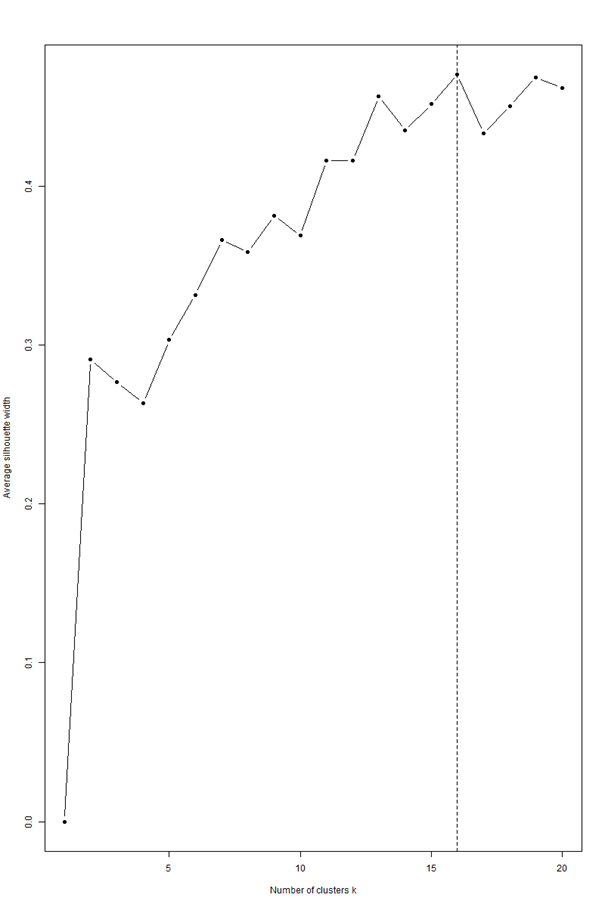
\includegraphics[width=0.6\linewidth]{aws.png} % Adjust the width as needed
    \caption{Average silhouette width (AWS) plot for hierarchical clustering 
	of all samples. The X-axis represents the number of clusters, and the Y-axis 
	is the average silhouette width. Cluster number $k = 16$ had the highest 
	average silhouette width. The closer the AWS value to 1, the more 
	well-separated and distinct clusters are, suggesting that the data 
	points within each cluster are similar to each other and dissimilar 
	to points in other clusters.}
	\label{fig:aws}
\end{figure*}

\begin{figure*}[] % Two column figure (notice the starred environment)
    \centering
    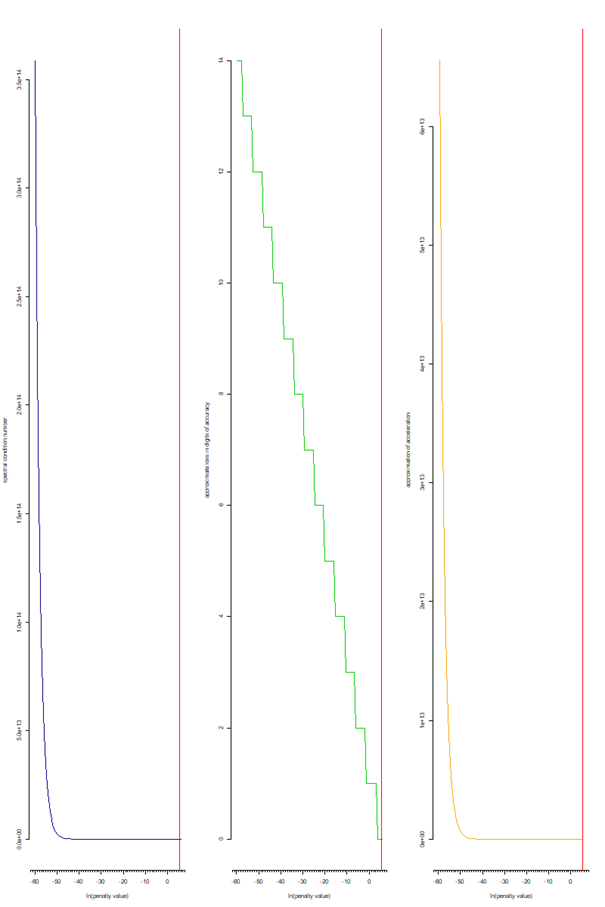
\includegraphics[width=0.8\linewidth]{CN_plot.png} % Adjust the width as needed
    \caption{A condition number plot with interpretational aids for class liver 30dpf. 
	Left-handed panel: the condition number plot. Middle panel:  the approximate loss 
	in digits of accuracy (for the operation of inversion) 
	plot \autocite{peeters2022a, peeters2020a}. Right-handed panel: 
	an approximation to the second-order derivative of the curvature in 
	the basic plot \autocite{peeters2022a, peeters2020a}. The vertical 
	red line corresponds to the previously computed optimal ridge penalty 
	for class liver 30dpf. The condition number of a matrix measures how 
	sensitive the matrix is to changes in its input – the numerically 
	stable matrix is favourable, indicating higher accuracy and 
	robustness. As seen in the left panel of the figure, the optimal 
	penalty parameter exceeded the minimal value of the penalty parameter; 
	the condition number remains relatively low and stable across the 
	variations of $\ln(\text{penalty value})$ before reaching the 
	estimated optimal penalty. An analogous pattern was present in 
	spectral condition number plots of all class-specific ridges}
	\label{fig:cnplot}
\end{figure*}

\clearpage
\subsection{\normalsize Differential networks}\label{diff-networks}
\begin{figure*}[ht] % Two column figure (notice the starred environment)
    \centering
    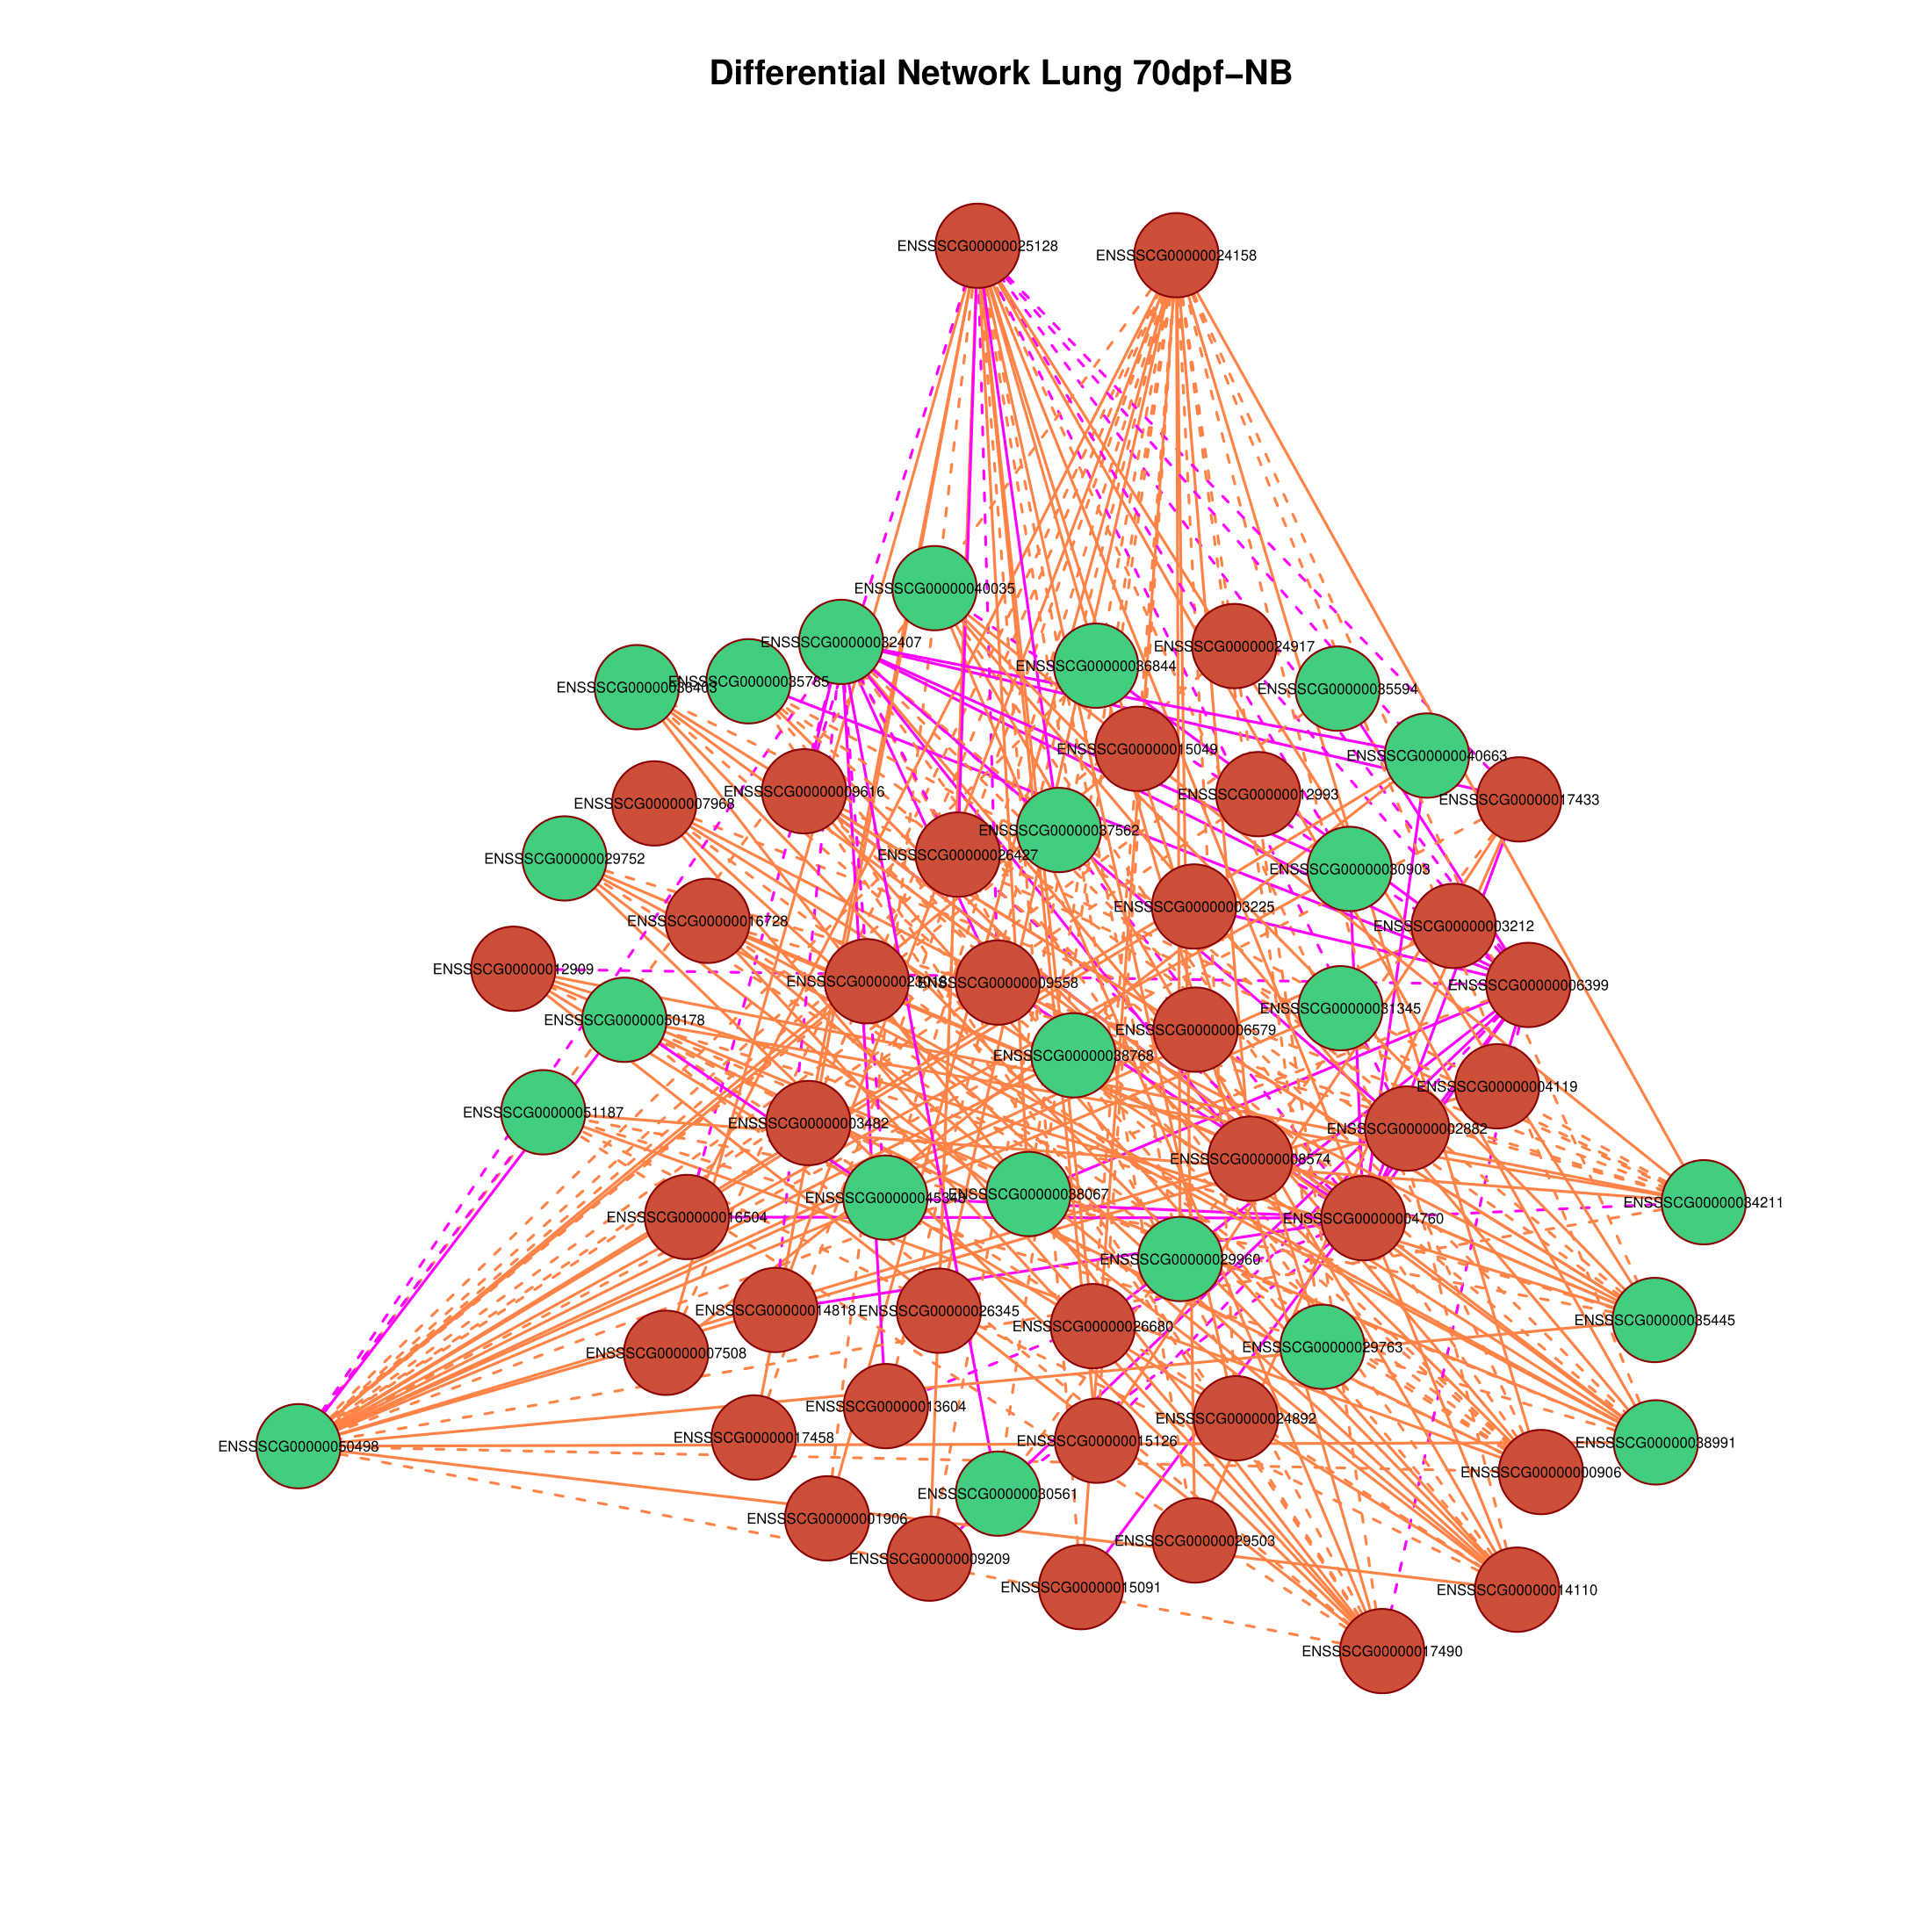
\includegraphics[width=\linewidth]{lung_70-NB.png} % Adjust the width as needed
    \caption{Differential network between lung stage 70dpf and lung stage NB. 
	Red nodes indicate up-regulated genes and green down-regulated genes. 
	Edges unique to class lung 70dpf are visualised in pink, while edges 
	unique to class lung NB are in orange. Solid edges correspond to 
	positive partial correlations, whereas dashed edges indicate negatively 
	weighted partial correlations.}
	\label{fig:lung70-NB}
\end{figure*}

\clearpage
\begin{figure*}[ht] % Two column figure (notice the starred environment)
    \centering
    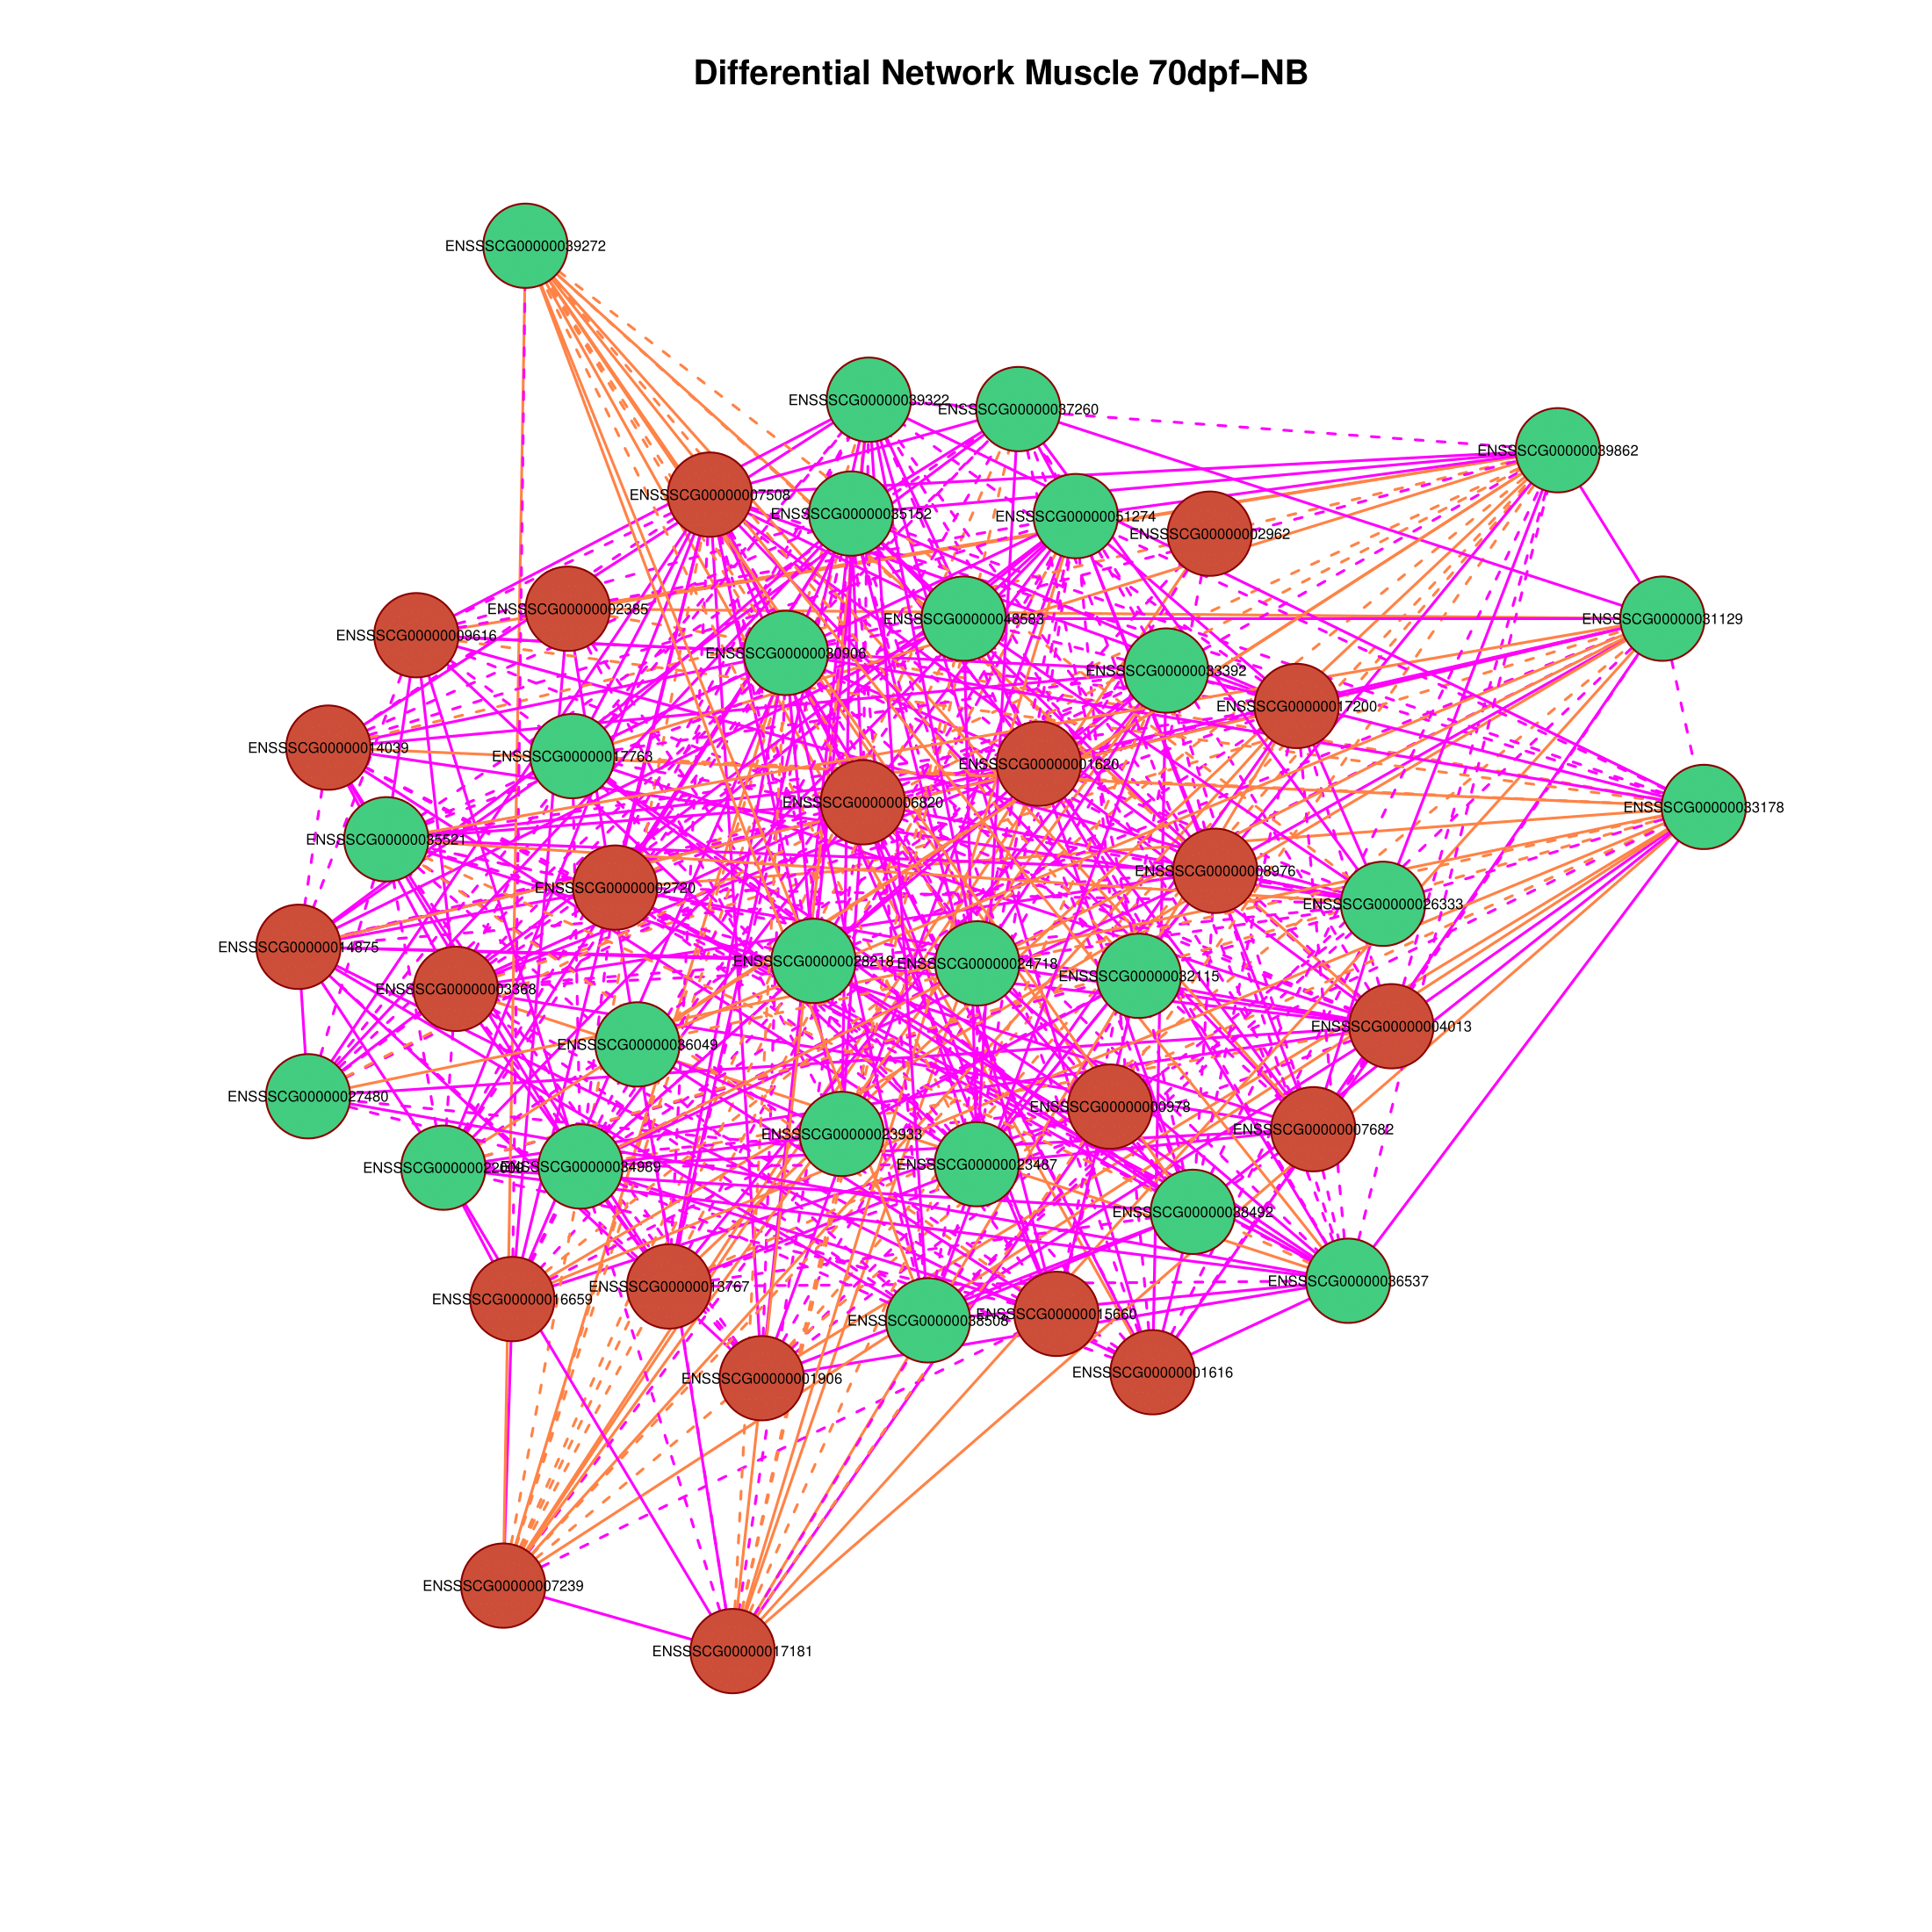
\includegraphics[width=\linewidth]{muscle_70-NB.png} % Adjust the width as needed
    \caption{Differential network between muscle stage 70dpf and muscle stage NB. 
	Red nodes indicate up-regulated genes and green down-regulated genes. 
	Edges unique to class muscle 70dpf are visualised in pink, while edges 
	unique to class muscle NB are in orange. Solid edges correspond to 
	positive partial correlations, whereas dashed edges indicate negatively 
	weighted partial correlations.}
	\label{fig:muscle70-NB}
\end{figure*}

\clearpage
\begin{figure*}[ht] % Two column figure (notice the starred environment)
    \centering
    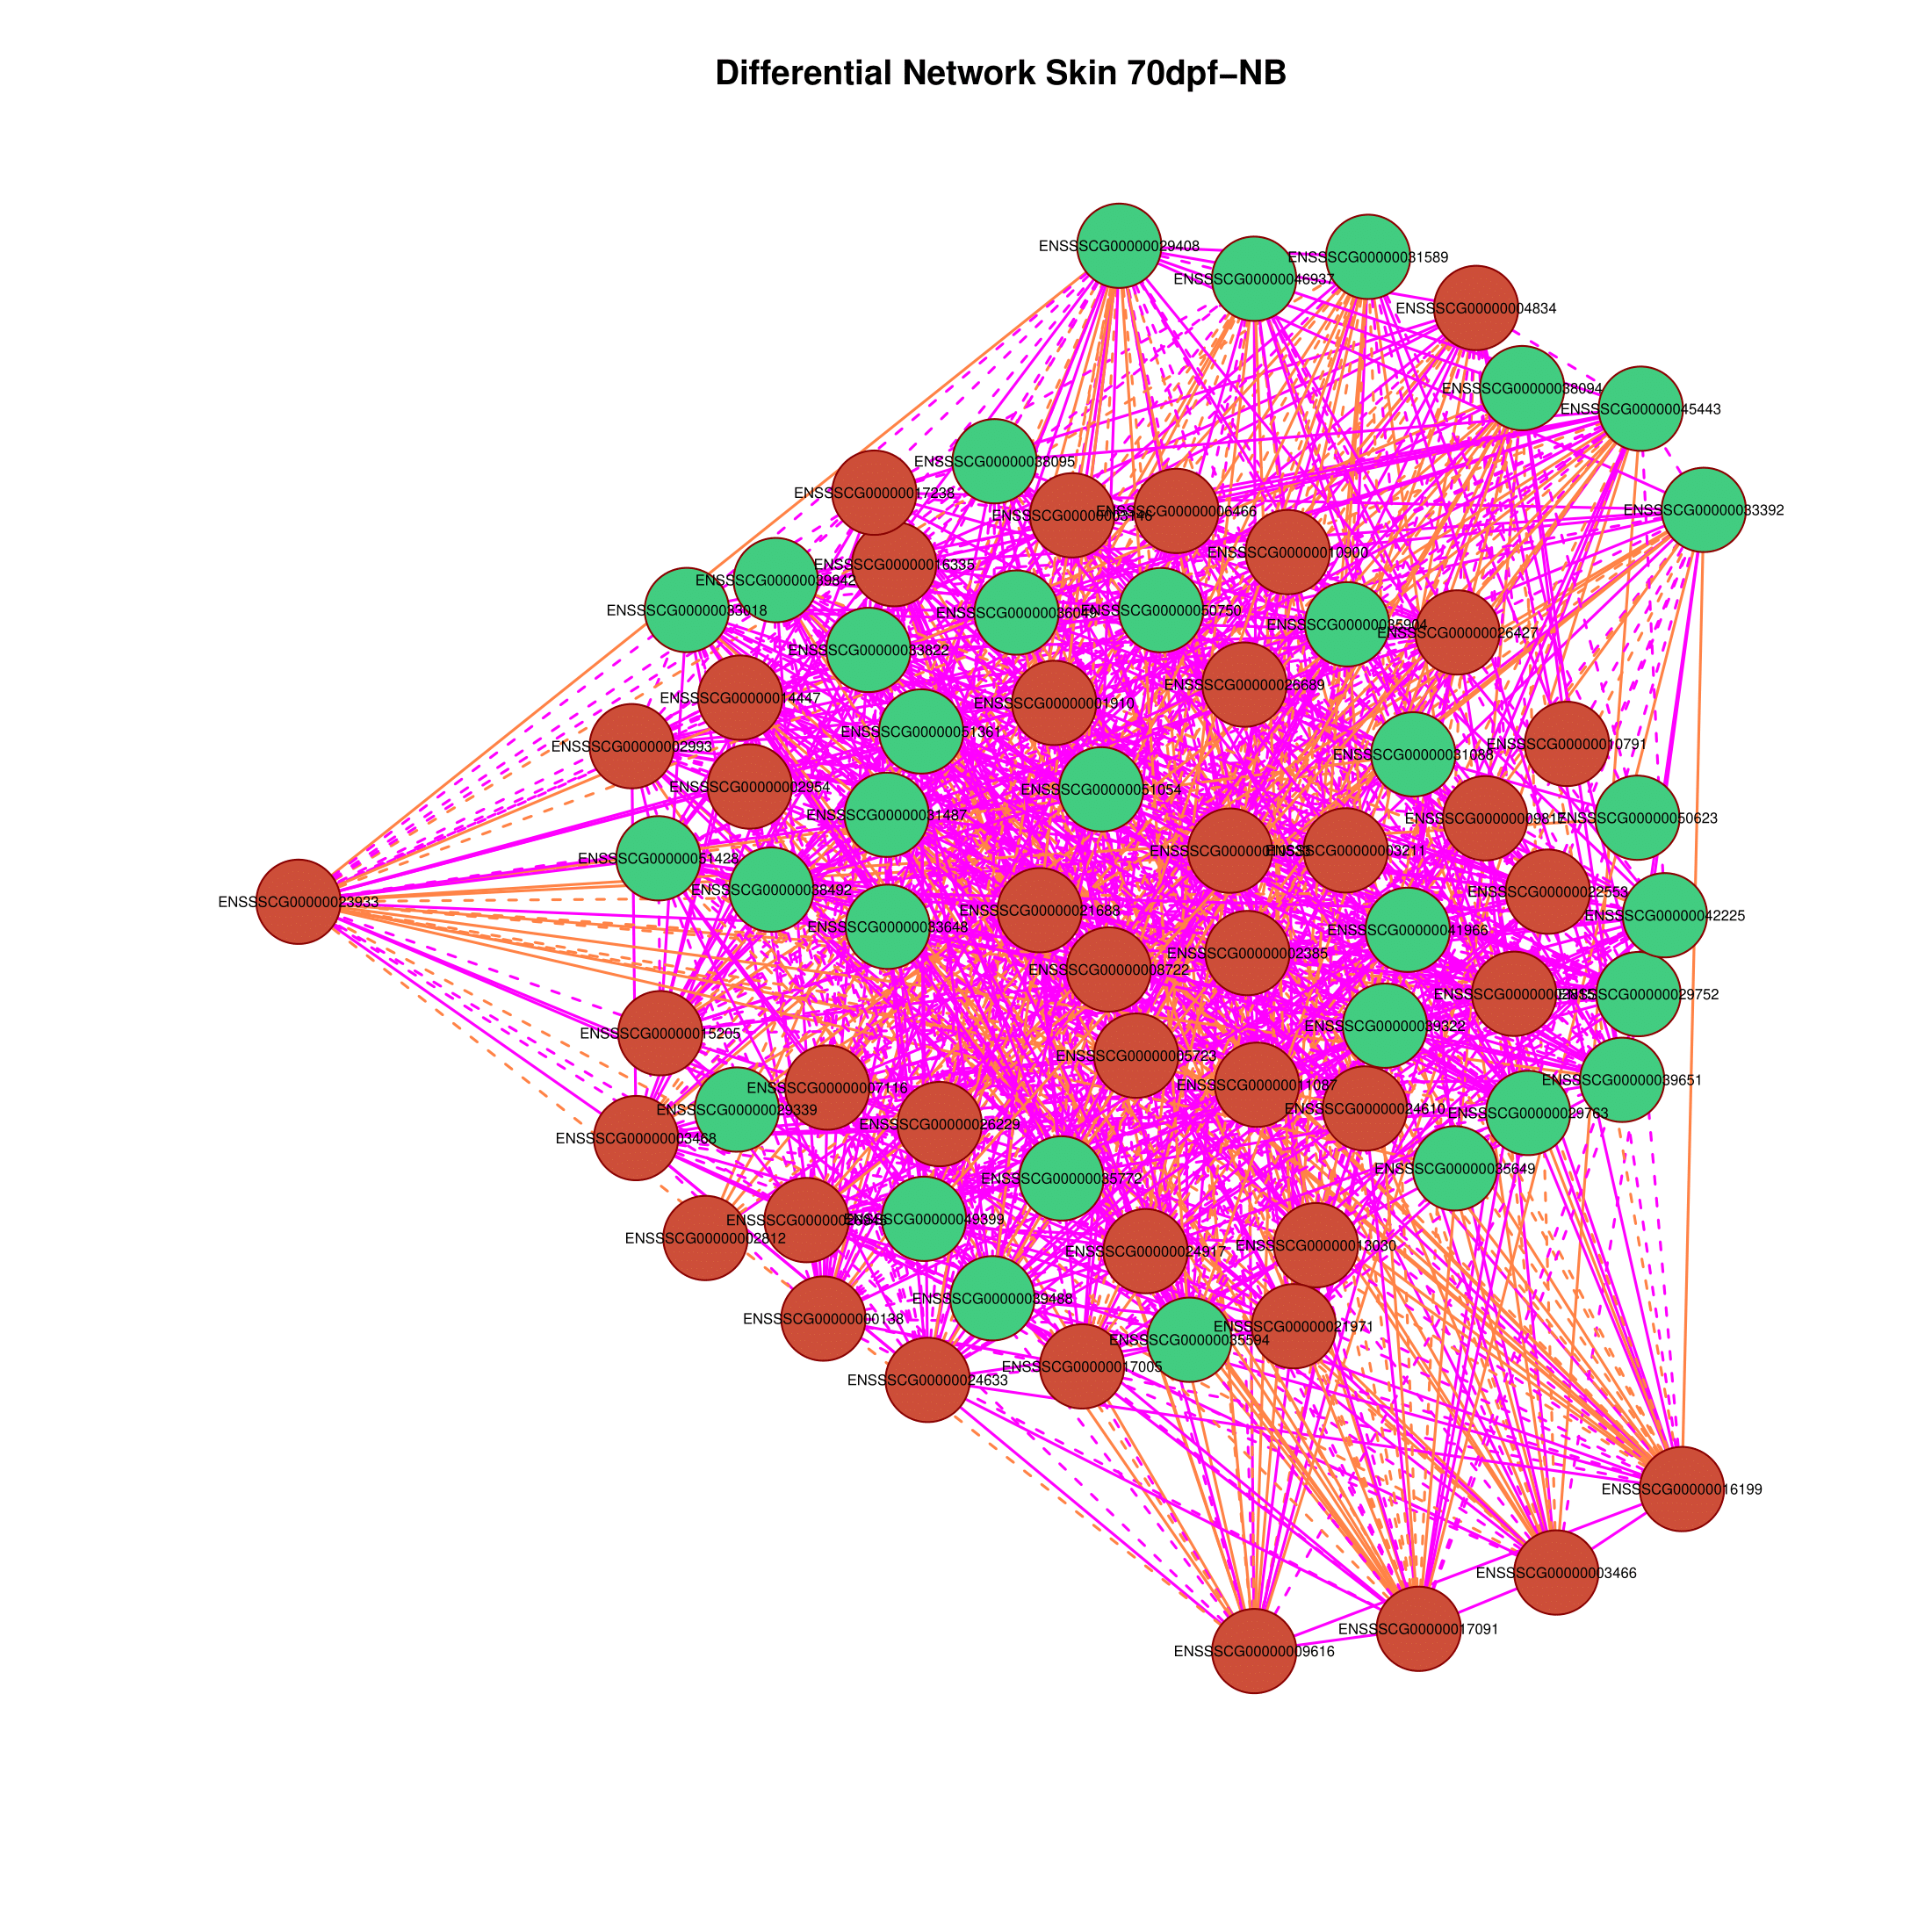
\includegraphics[width=\linewidth]{skin_70-NB.png} % Adjust the width as needed
    \caption{Differential network between skin stage 70dpf and skin stage NB. 
	Red nodes indicate up-regulated genes and green down-regulated genes. 
	Edges unique to class skin 70dpf are visualised in pink, while edges 
	unique to class skin NB are in orange. Solid edges correspond to 
	positive partial correlations, whereas dashed edges indicate negatively 
	weighted partial correlations.}
	\label{fig:skin70-NB}
\end{figure*}

\clearpage
\subsection{\normalsize Community detection}\label{comm-det}
\begin{figure*}[ht] % Two column figure (notice the starred environment)
    \centering
    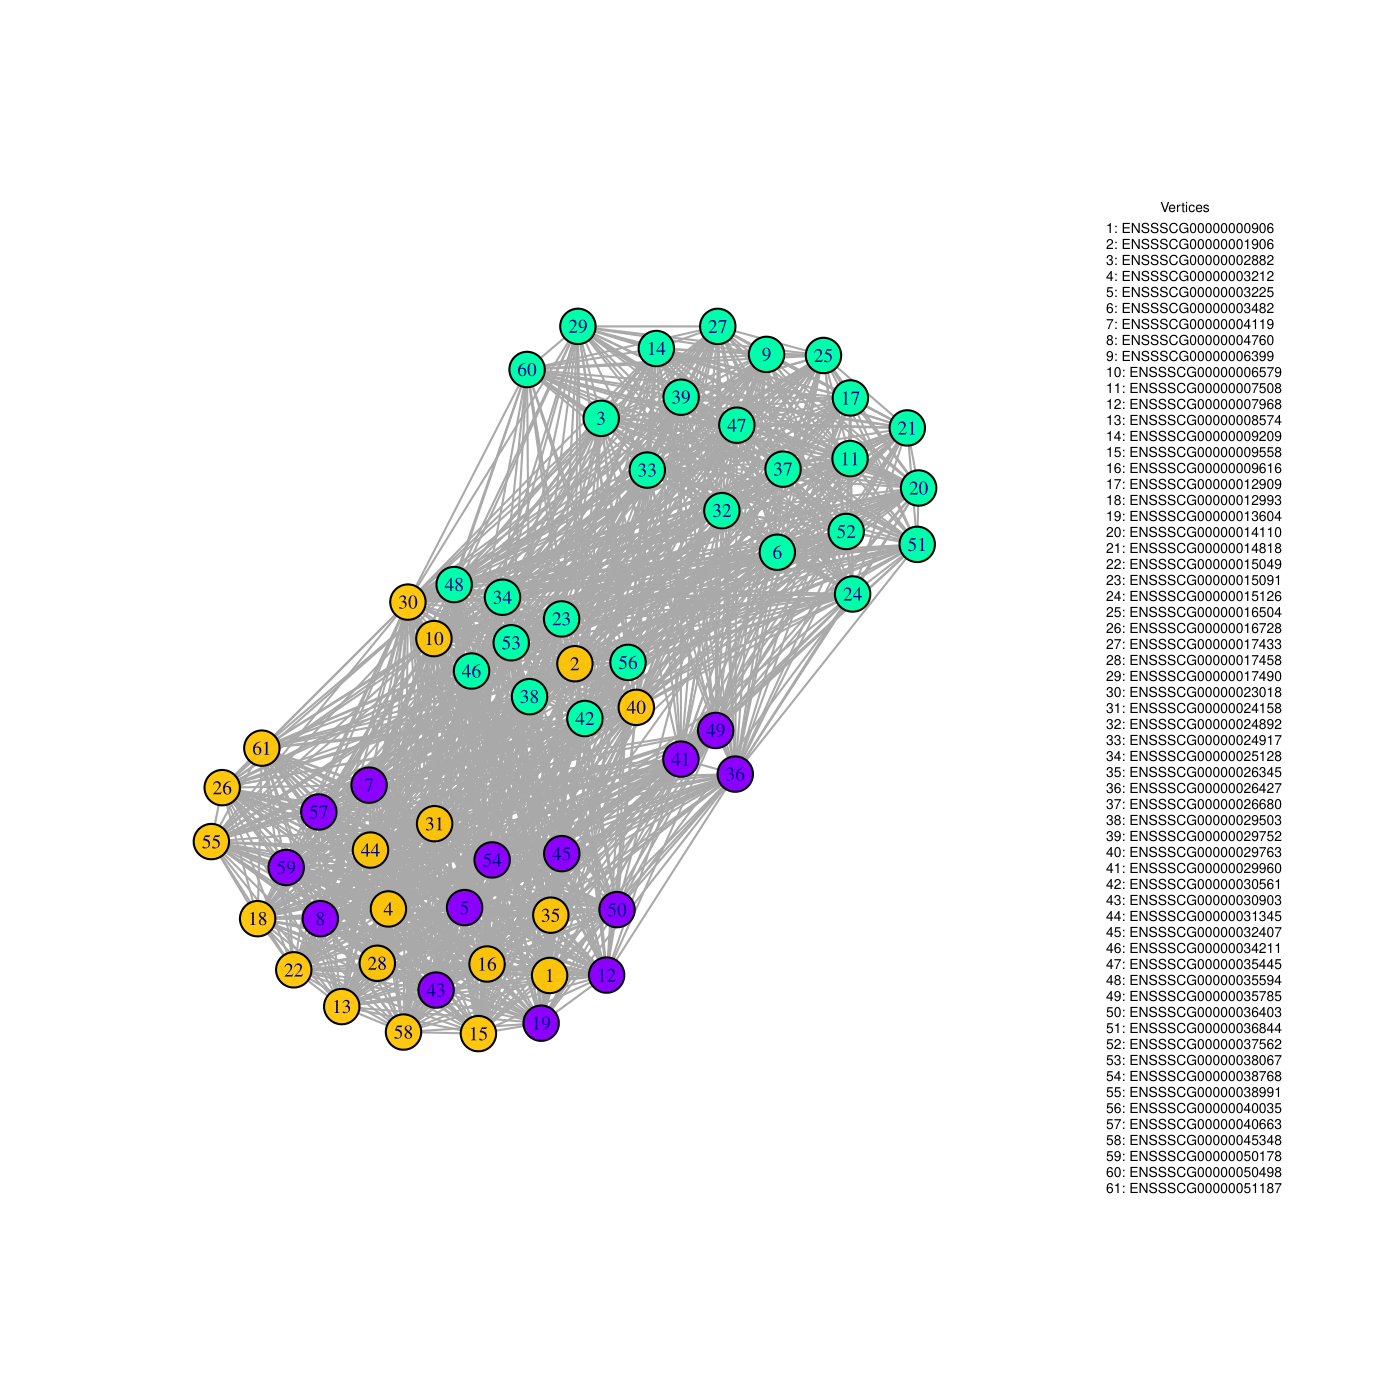
\includegraphics[width=\linewidth]{communities_liver30.png} % Adjust the width as needed
    \caption{Communities detected for liver 30dpf with 
	the \texttt{cluster\_fluid\_communities()} function from the igraph R package.
	Each community is assigned a different colour. The legend on the right
	provides the encoding of Ensembl gene IDs in the network.}
	\label{fig:com-liv30}
\end{figure*}

\clearpage
\begin{figure*}[ht] % Two column figure (notice the starred environment)
    \centering
    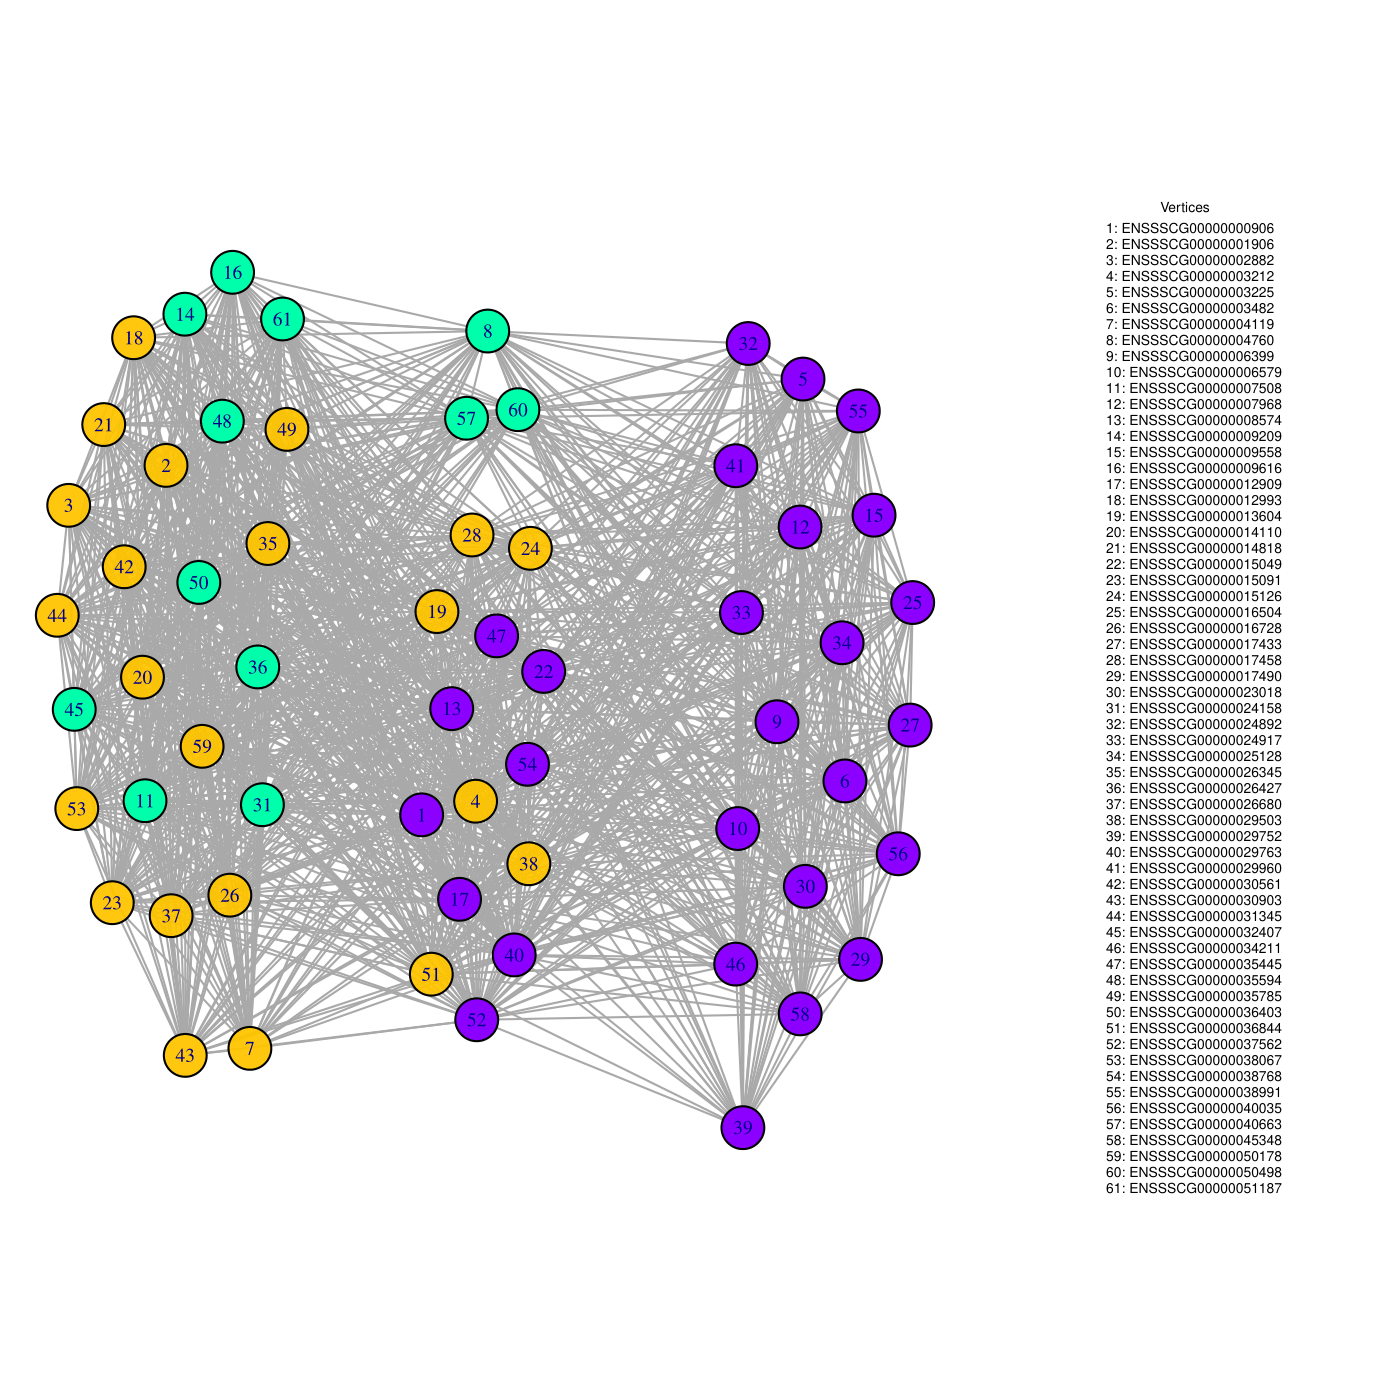
\includegraphics[width=\linewidth]{communities_liver70.png} % Adjust the width as needed
    \caption{Communities detected for liver 70dpf with 
	the \texttt{cluster\_fluid\_communities()} function from the igraph R package.
	Each community is assigned a different colour. The legend on the right
	provides the encoding of Ensembl gene IDs in the network.}
	\label{fig:com-liv70}
\end{figure*}

\clearpage
\begin{figure*}[ht] % Two column figure (notice the starred environment)
    \centering
    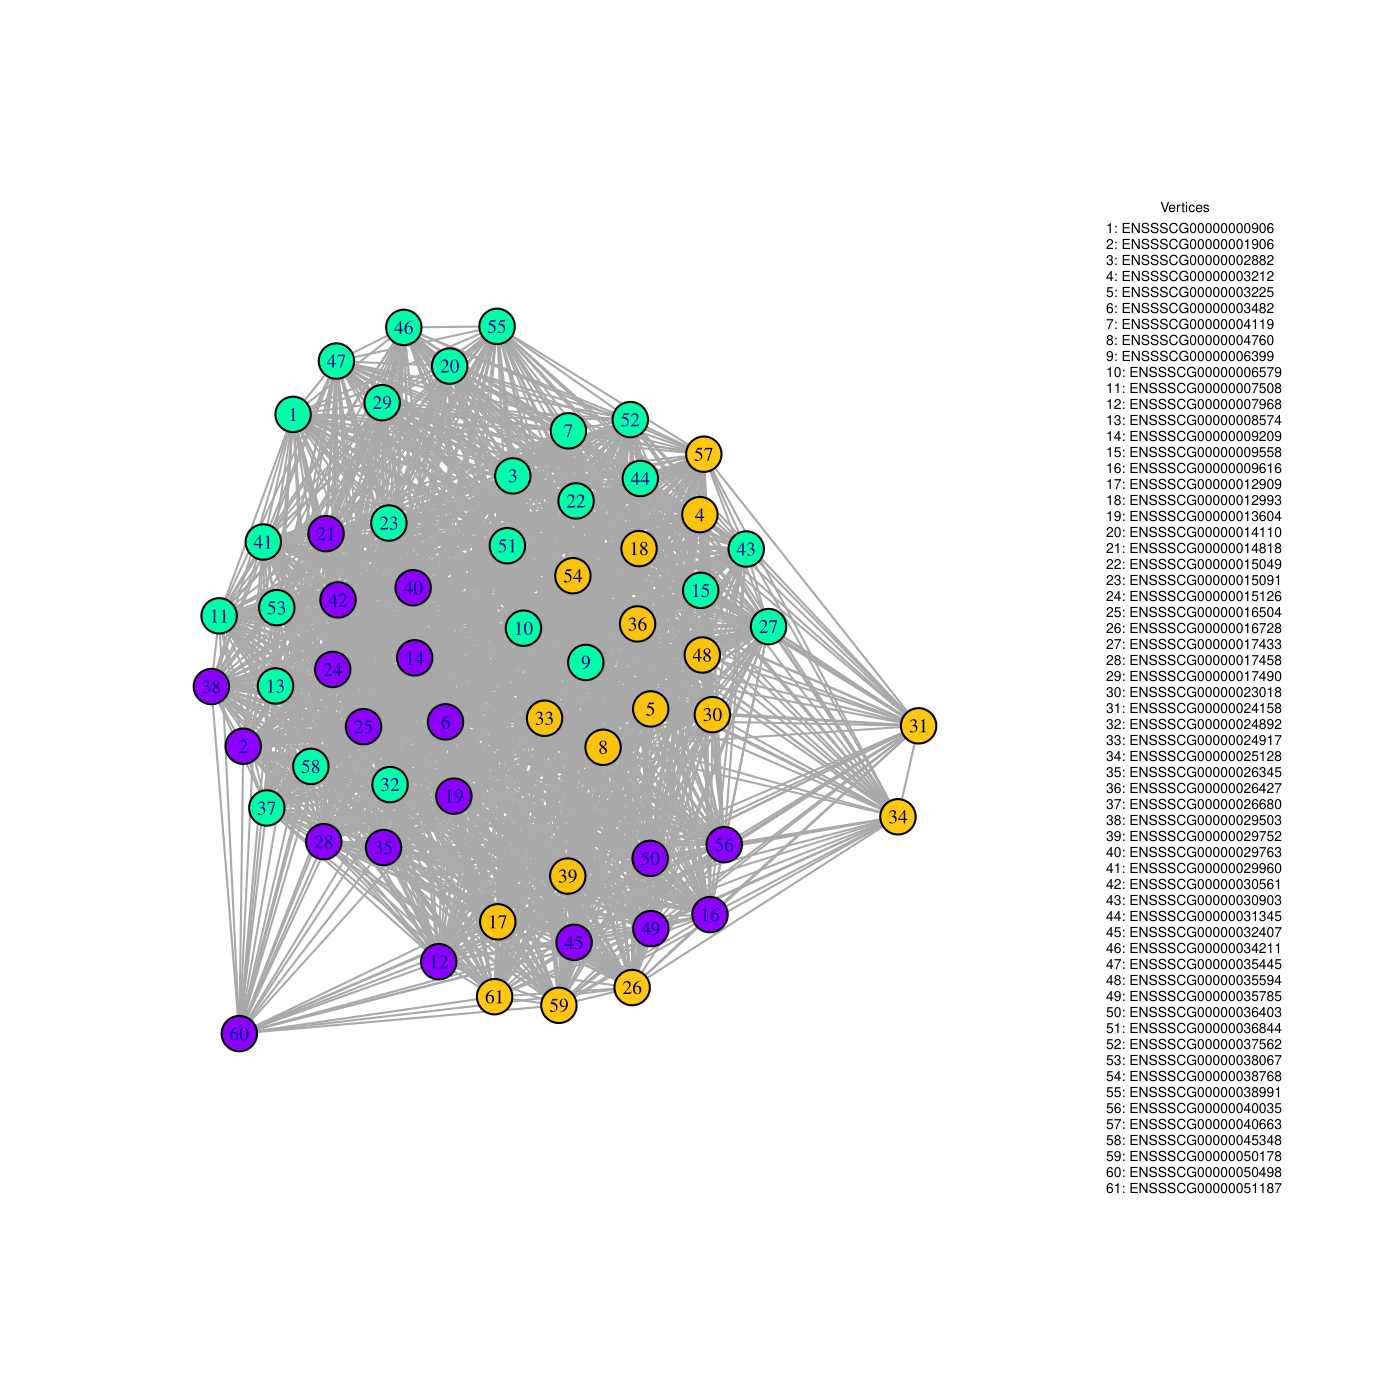
\includegraphics[width=\linewidth]{communities_lung70.png} % Adjust the width as needed
    \caption{Communities detected for lung 70dpf with 
	the \texttt{cluster\_fluid\_communities()} function from the igraph R package.
	Each community is assigned a different colour. The legend on the right
	provides the encoding of Ensembl gene IDs in the network.}
	\label{fig:com-lung70}
\end{figure*}

\clearpage
\begin{figure*}[ht] % Two column figure (notice the starred environment)
    \centering
    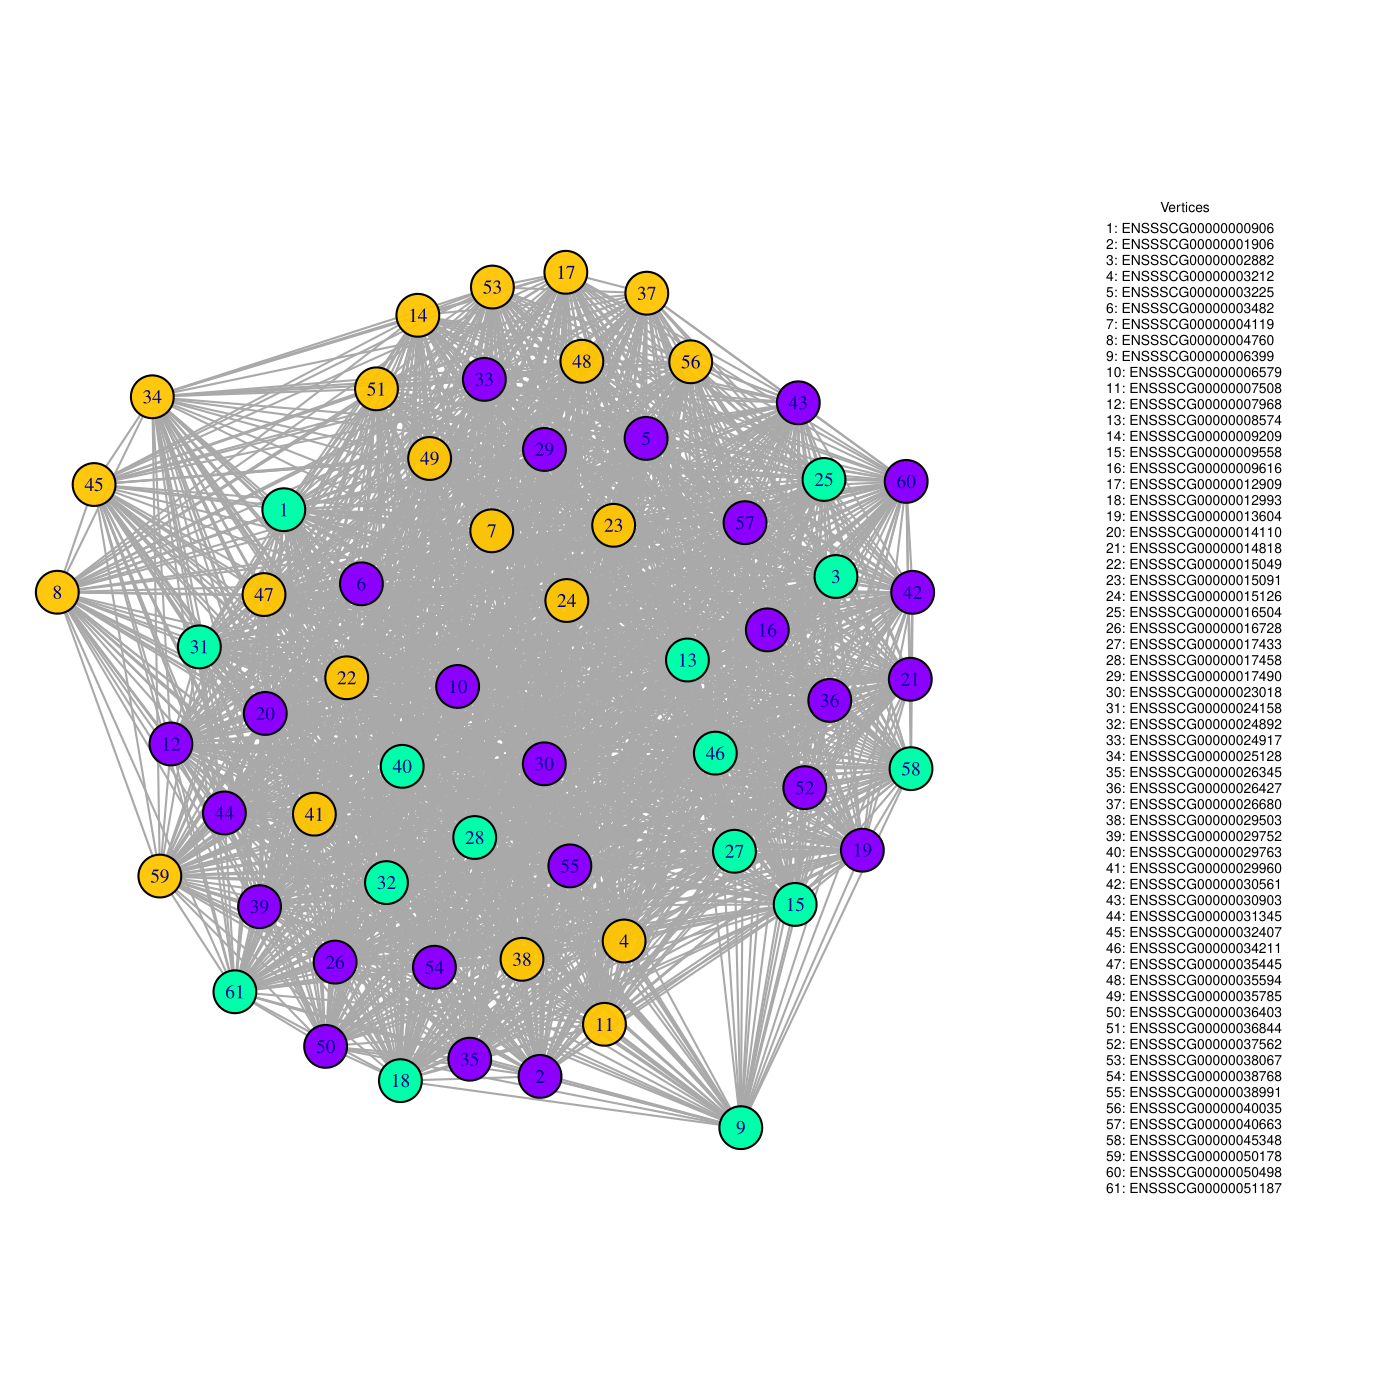
\includegraphics[width=\linewidth]{communities_lungNB.png} % Adjust the width as needed
    \caption{Communities detected for lung NB with 
	the \texttt{cluster\_fluid\_communities()} function from the igraph R package.
	Each community is assigned a different colour. The legend on the right
	provides the encoding of Ensembl gene IDs in the network.}
	\label{fig:com-lungNB}
\end{figure*}

\clearpage
\begin{figure*}[ht] % Two column figure (notice the starred environment)
    \centering
    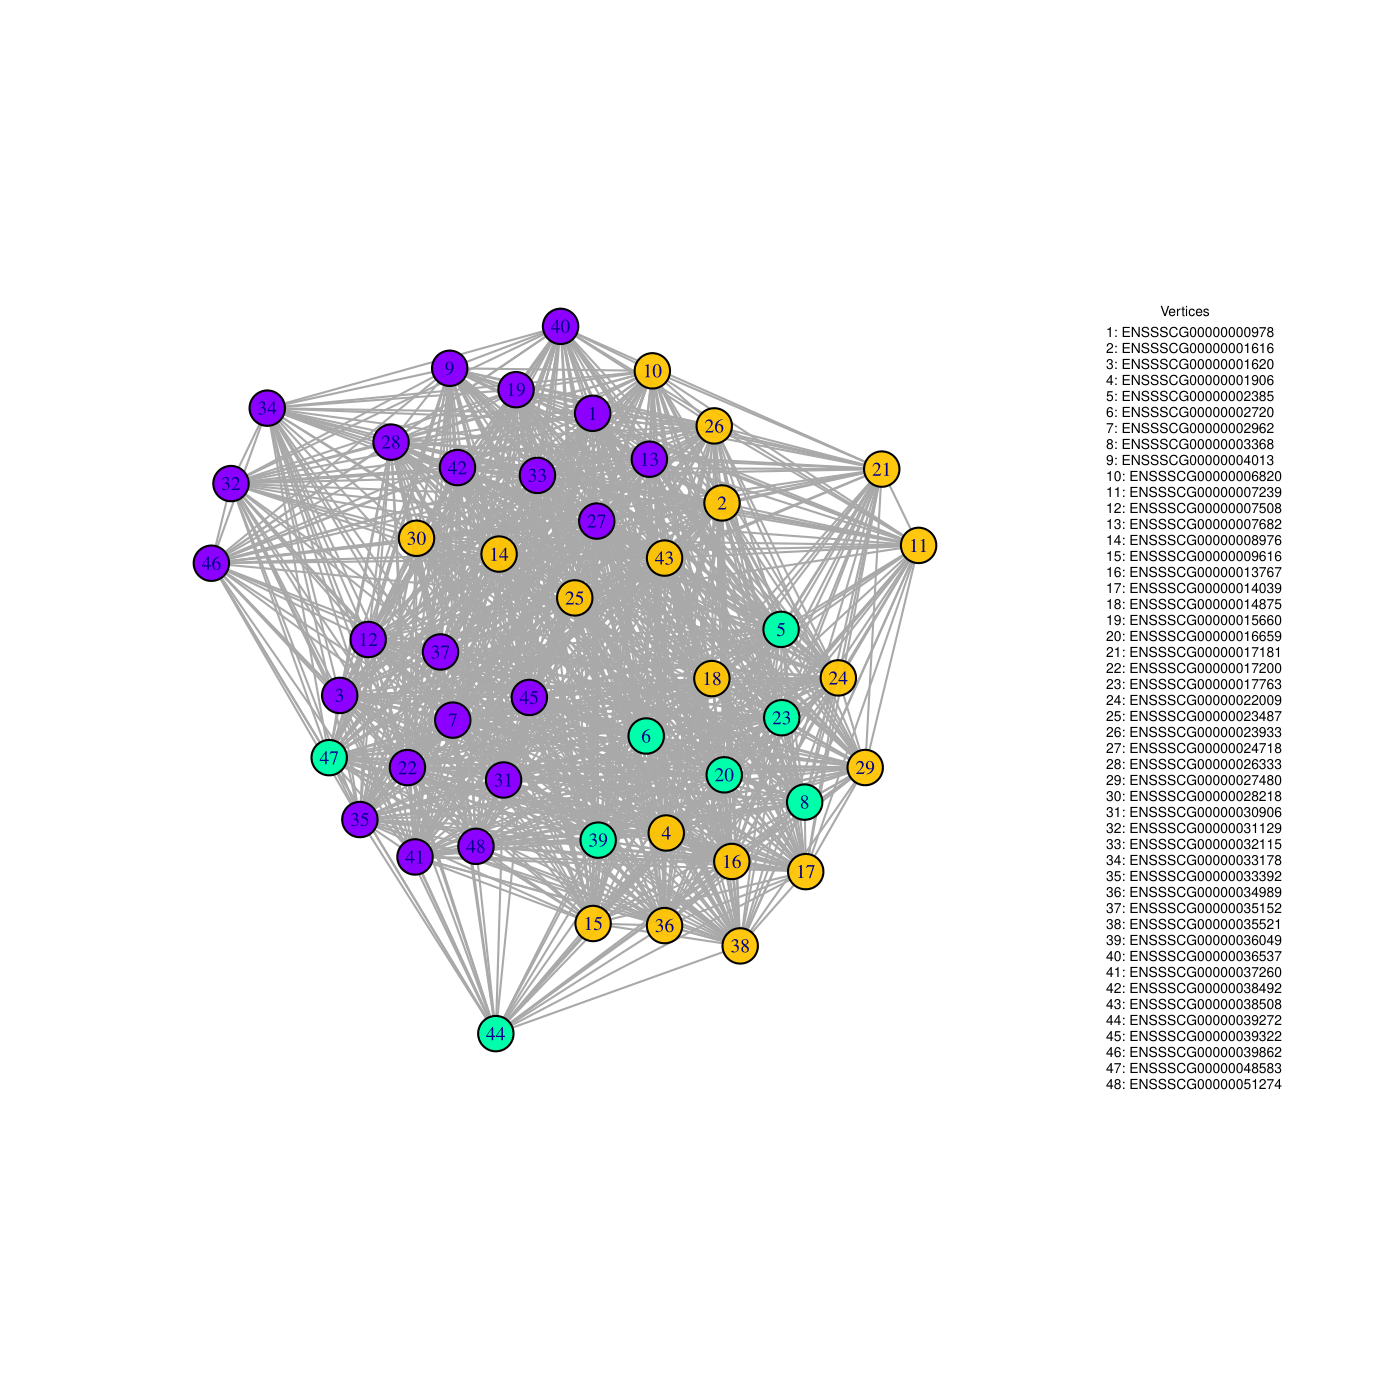
\includegraphics[width=\linewidth]{communities_muscle70.png} % Adjust the width as needed
    \caption{Communities detected for muscle 70dpf with 
	the \texttt{cluster\_fluid\_communities()} function from the igraph R package.
	Each community is assigned a different colour. The legend on the right
	provides the encoding of Ensembl gene IDs in the network.}
	\label{fig:com-muscle70}
\end{figure*}

\clearpage
\begin{figure*}[ht] % Two column figure (notice the starred environment)
    \centering
    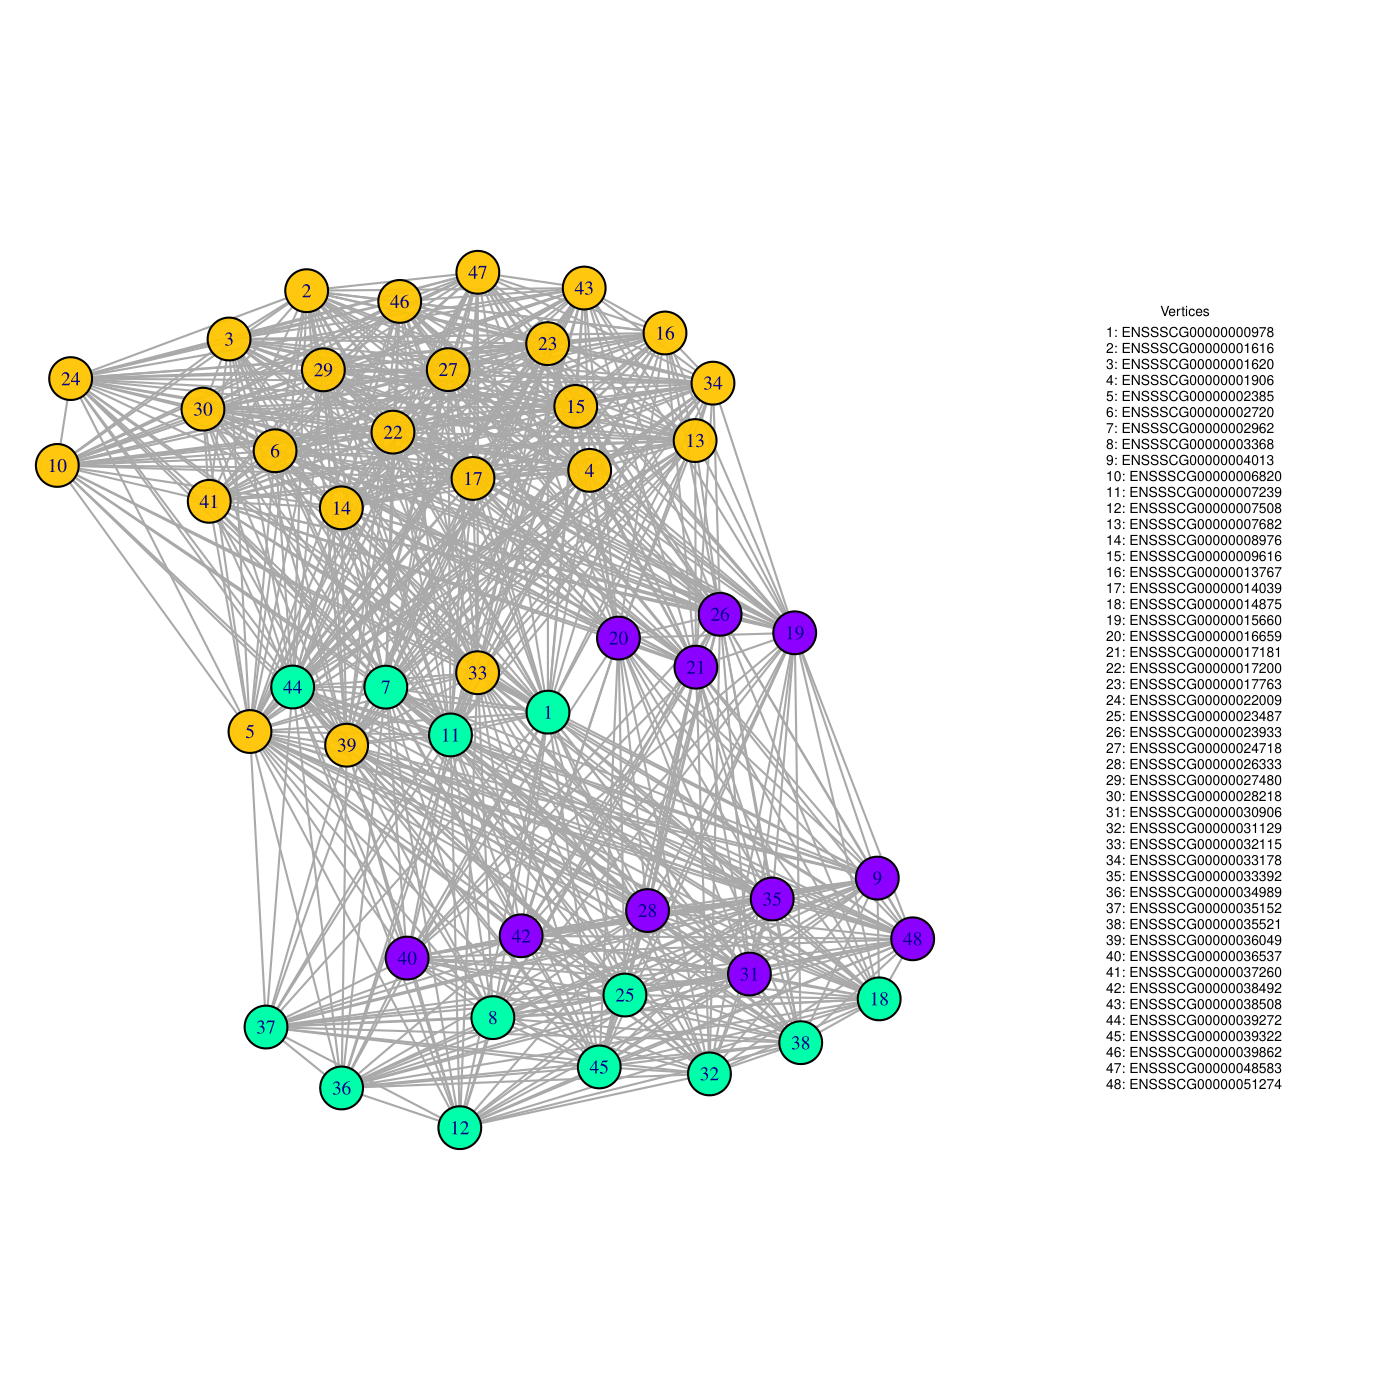
\includegraphics[width=\linewidth]{communities_muscleNB.png} % Adjust the width as needed
    \caption{Communities detected for muscle NB with 
	the \texttt{cluster\_fluid\_communities()} function from the igraph R package.
	Each community is assigned a different colour. The legend on the right
	provides the encoding of Ensembl gene IDs in the network.}
	\label{fig:com-muscleNB}
\end{figure*}

\clearpage
\begin{figure*}[ht] % Two column figure (notice the starred environment)
    \centering
    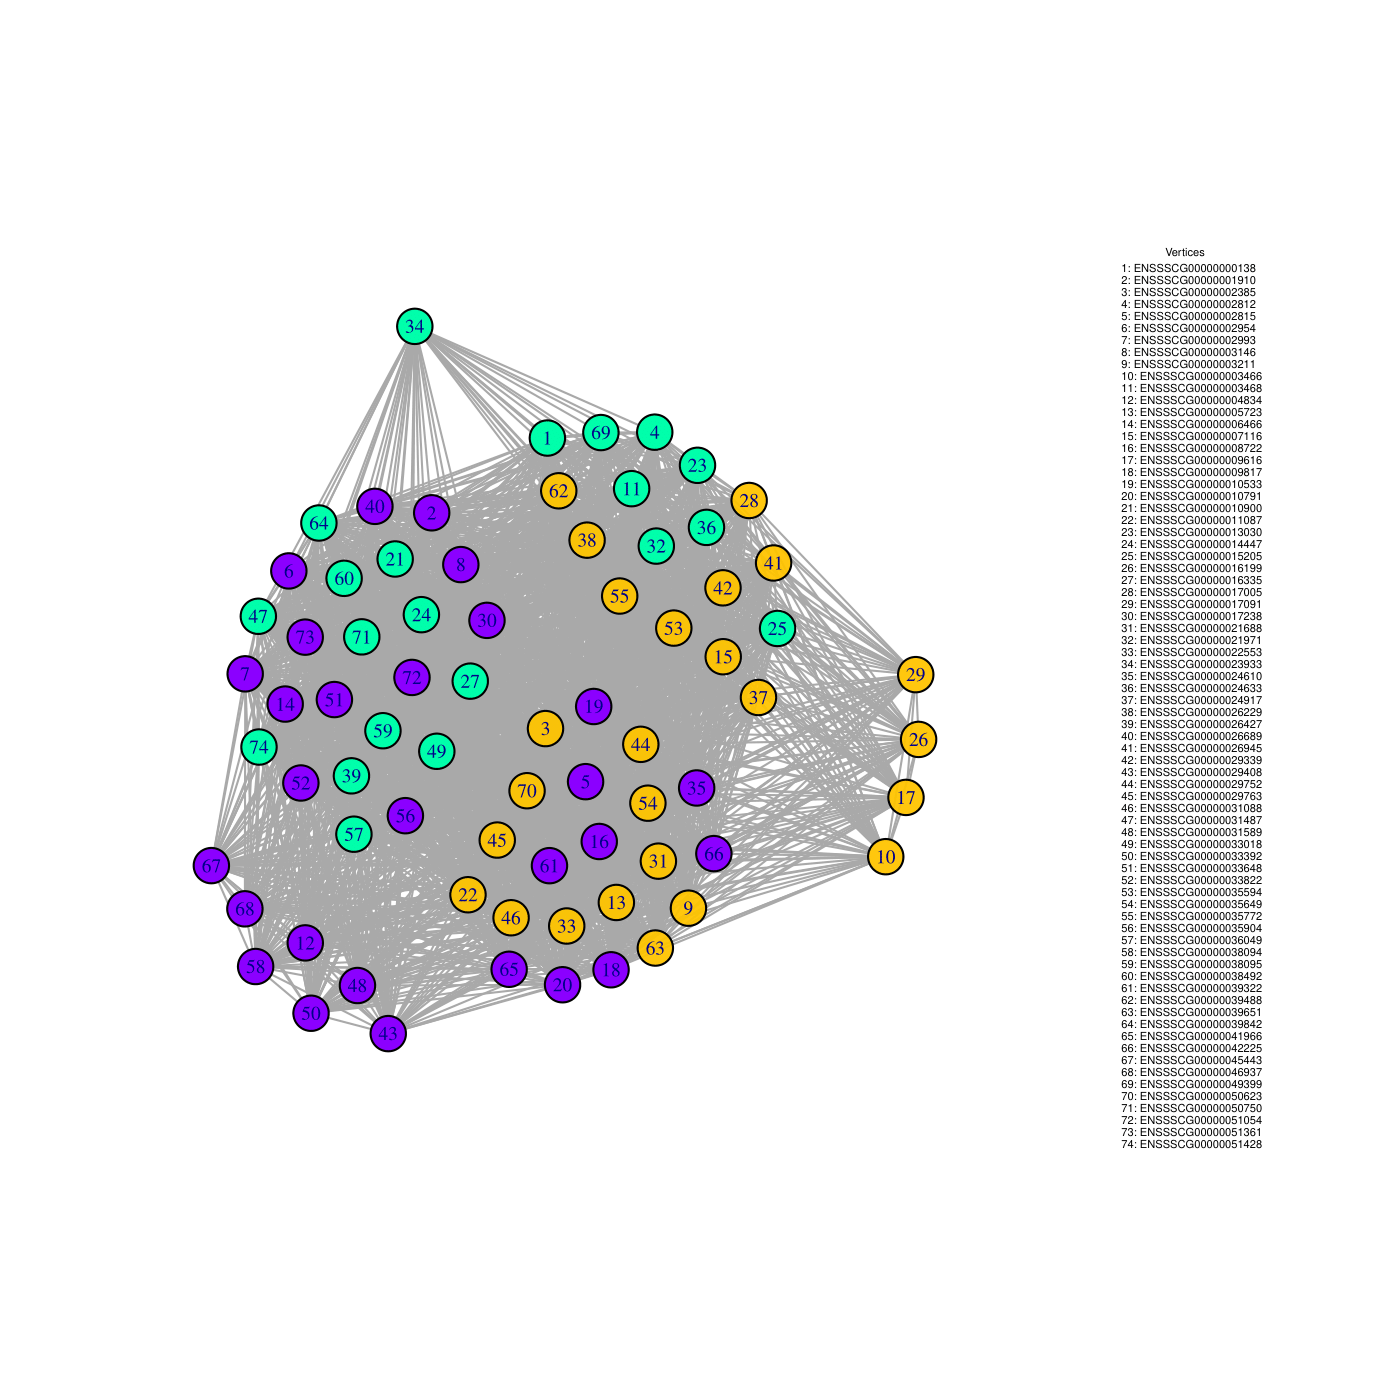
\includegraphics[width=\linewidth]{communities_skin70.png} % Adjust the width as needed
    \caption{Communities detected for skin 70dpf with 
	the \texttt{cluster\_fluid\_communities()} function from the igraph R package.
	Each community is assigned a different colour. The legend on the right
	provides the encoding of Ensembl gene IDs in the network.}
	\label{fig:com-skin70}
\end{figure*}

\clearpage
\begin{figure*}[ht] % Two column figure (notice the starred environment)
    \centering
    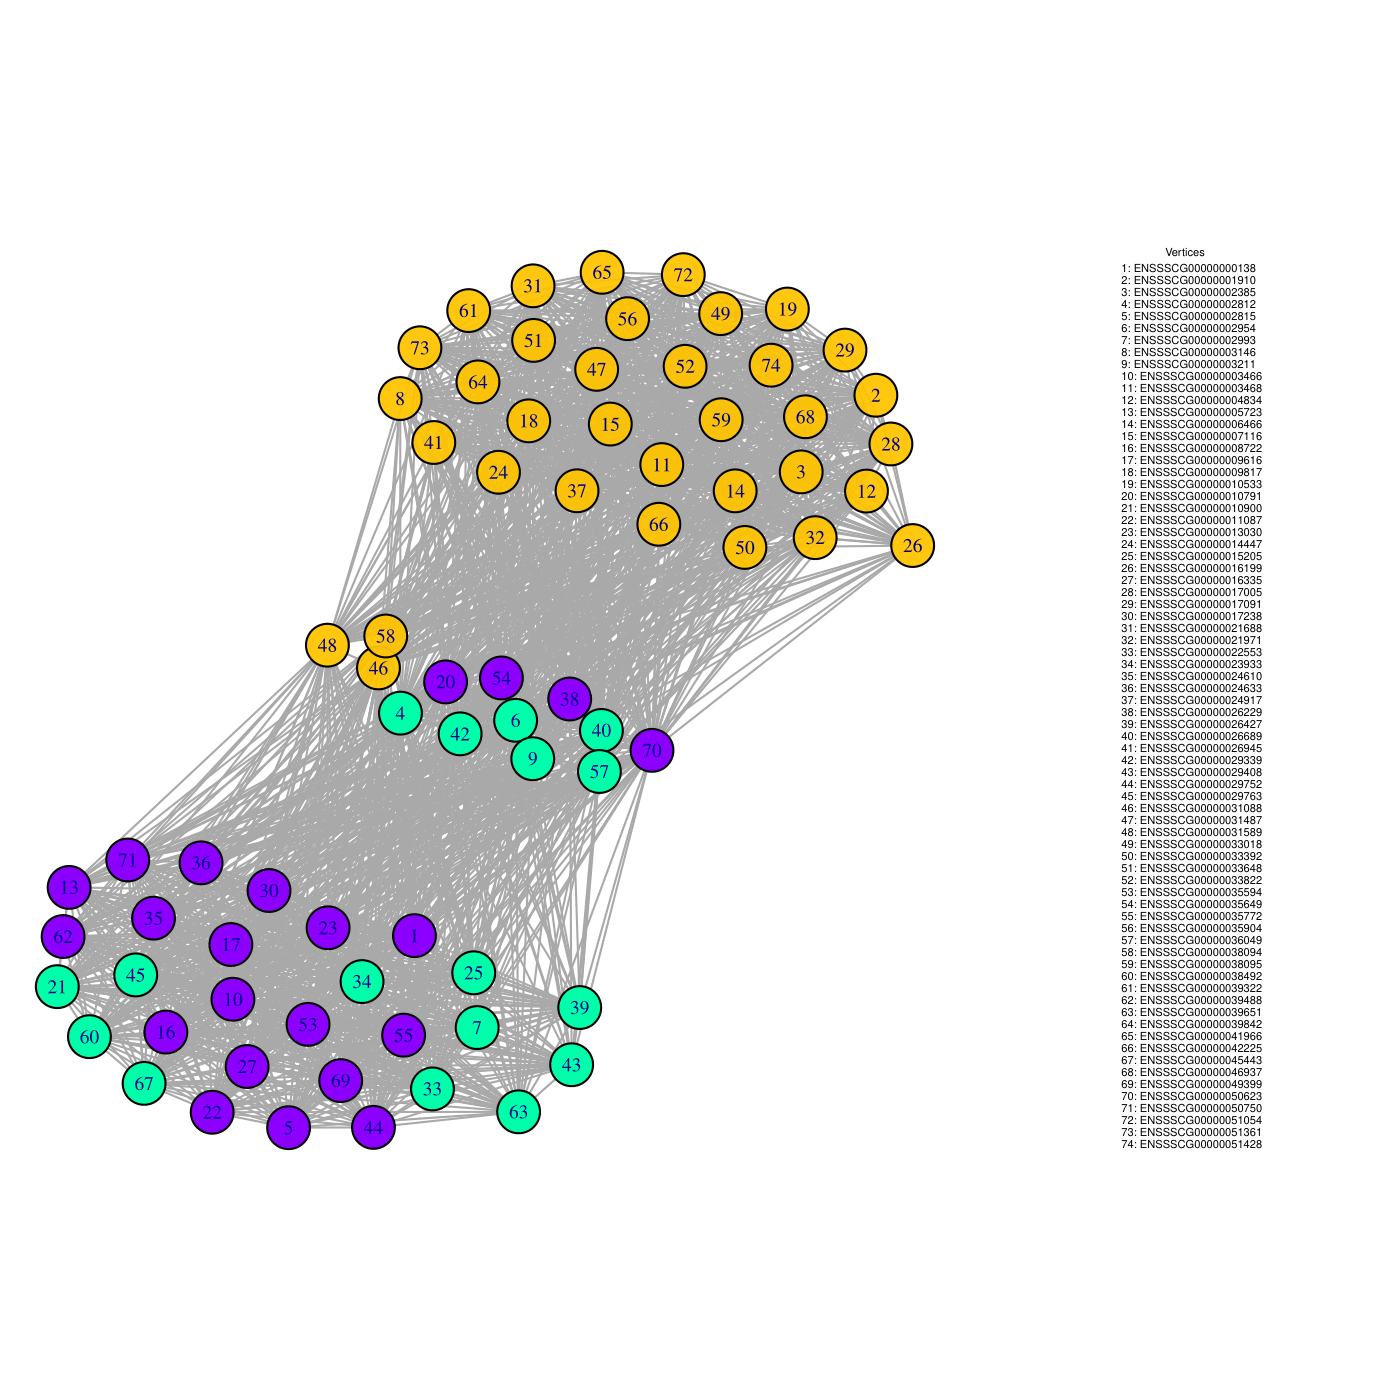
\includegraphics[width=\linewidth]{communities_skinNB.png} % Adjust the width as needed
    \caption{Communities detected for skin NB with 
	the \texttt{cluster\_fluid\_communities()} function from the igraph R package.
	Each community is assigned a different colour. The legend on the right
	provides the encoding of Ensembl gene IDs in the network.}
	\label{fig:com-skinNB}
\end{figure*}

\clearpage
\subsection{\normalsize Network analysis}\label{net-anal}
\begin{table}[htbp]
    \centering
	\caption{Enrichr gene set enrichment analysis results for 18 genes with the highest betweenness centrality in the liver 30dpf network. Enrichment was conducted using Descartes Cell Types and Tissue 2021.}
	\label{tab:liv30enr}
	\resizebox{\textwidth}{!}{%
	\begin{tabular}{clrrrr}
	\hline
	\rowcolor[HTML]{FFFFFF} 
	\textbf{Index} & \textbf{Name} & \textbf{P-value} & \textbf{Adjusted p-value} & \textbf{Odds Ratio} & \textbf{Combined score} \\ \hline
	\rowcolor[HTML]{F9F9F9} 
	1 & Ductal cells in Pancreas & 0.003099 & 0.03470 & 28.06 & 162.11 \\
	\rowcolor[HTML]{FFFFFF} 
	2 & Lymphoid cells in Liver & 0.003305 & 0.03470 & 27.14 & 155.01 \\
	\rowcolor[HTML]{F9F9F9} 
	3 & Corneal and conjunctival epithelial cells in Eye & 0.02106 & 0.1200 & 10.15 & 39.17 \\
	\rowcolor[HTML]{FFFFFF} 
	4 & Endocardial cells in Heart & 0.02286 & 0.1200 & 47.97 & 181.23 \\
	\rowcolor[HTML]{F9F9F9} 
	5 & Vascular endothelial cells in Lung & 0.03716 & 0.1451 & 28.93 & 95.26 \\
	\rowcolor[HTML]{FFFFFF} 
	6 & Hepatoblasts in Liver & 0.04145 & 0.1451 & 6.97 & 22.17 \\
	\rowcolor[HTML]{F9F9F9} 
	7 & Squamous epithelial cells in Stomach & 0.04925 & 0.1478 & 21.58 & 64.96 \\
	\rowcolor[HTML]{FFFFFF} 
	8 & MUC13 DMBT1 positive cells in Stomach & 0.06582 & 0.1580 & 15.94 & 43.36 \\
	\rowcolor[HTML]{F9F9F9} 
	9 & Vascular endothelial cells in Placenta & 0.07107 & 0.1580 & 14.71 & 38.88 \\
	\rowcolor[HTML]{FFFFFF} 
	10 & Lymphoid cells in Spleen & 0.08018 & 0.1580 & 12.95 & 32.68 \\ \hline
	\end{tabular}%
	}
	\end{table}

\begin{table}[htbp]
	\caption{Enrichr gene set enrichment analysis results for 17 genes with the highest betweenness centrality in the liver 70dpf network. Enrichment was conducted using Descartes Cell Types and Tissue 2021.}
	\label{tab:liv70enr}
	\resizebox{\textwidth}{!}{%
	\begin{tabular}{clrrrr}
	\hline
	\rowcolor[HTML]{FFFFFF} 
	\textbf{Index} & \textbf{Name} & \textbf{P-value} & \textbf{Adjusted p-value} & \textbf{Odds Ratio} & \textbf{Combined score} \\ \hline
	\rowcolor[HTML]{F9F9F9} 
	1 & Lymphoid cells in Heart & 0.003863 & 0.04758 & 24.54 & 136.34 \\
	\rowcolor[HTML]{FFFFFF} 
	2 & Lymphoid cells in Lung & 0.007058 & 0.04758 & 17.87 & 88.52 \\
	\rowcolor[HTML]{F9F9F9} 
	3 & Lymphoid cells in Pancreas & 0.007241 & 0.04758 & 17.63 & 86.88 \\
	\rowcolor[HTML]{FFFFFF} 
	4 & Lymphoid cells in Intestine & 0.007613 & 0.04758 & 17.17 & 83.74 \\
	\rowcolor[HTML]{F9F9F9} 
	5 & Lymphoid cells in Adrenal & 0.009706 & 0.04853 & 15.09 & 69.95 \\
	\rowcolor[HTML]{FFFFFF} 
	6 & Antigen presenting cells in Thymus & 0.01333 & 0.05555 & 12.74 & 55.00 \\
	\rowcolor[HTML]{F9F9F9} 
	7 & Lymphoid cells in Kidney & 0.02013 & 0.07190 & 10.19 & 39.81 \\
	\rowcolor[HTML]{FFFFFF} 
	8 & Lymphoid cells in Stomach & 0.06987 & 0.2051 & 14.81 & 39.40 \\
	\rowcolor[HTML]{F9F9F9} 
	9 & Myeloid cells in Stomach & 0.07384 & 0.2051 & 13.97 & 36.41 \\
	\rowcolor[HTML]{FFFFFF} 
	10 & SATB2 LRRC7 positive cells in Heart & 0.1042 & 0.2605 & 9.69 & 21.92 \\ \hline
	\end{tabular}%
	}
	\end{table}

\begin{table}[htbp]
	\caption{Enrichr gene set enrichment analysis results for 19 genes with the highest betweenness centrality in the lung 70dpf network. Enrichment was conducted using Descartes Cell Types and Tissue 2021.}
	\label{tab:lung70enr}
	\resizebox{\textwidth}{!}{%
	\begin{tabular}{clrrrr}
	\hline
	\rowcolor[HTML]{FFFFFF} 
	\textbf{Index} & \textbf{Name} & \textbf{P-value} & \textbf{Adjusted p-value} & \textbf{Odds Ratio} & \textbf{Combined score} \\ \hline
	\rowcolor[HTML]{F9F9F9} 
	1 & Ductal cells in Pancreas & 0.005711 & 0.1428 & 19.80 & 102.29 \\
	\rowcolor[HTML]{FFFFFF} 
	2 & PAEP MECOM positive cells in Placenta & 0.01232 & 0.1541 & 13.16 & 57.87 \\
	\rowcolor[HTML]{F9F9F9} 
	3 & Vascular endothelial cells in Lung & 0.05009 & 0.2805 & 20.89 & 62.54 \\
	\rowcolor[HTML]{FFFFFF} 
	4 & Squamous epithelial cells in Stomach & 0.06626 & 0.2805 & 15.58 & 42.28 \\
	\rowcolor[HTML]{F9F9F9} 
	5 & Lymphoid cells in Heart & 0.09953 & 0.2805 & 10.13 & 23.37 \\
	\rowcolor[HTML]{FFFFFF} 
	6 & IGFBP1 DKK1 positive cells in Placenta & 0.1106 & 0.2805 & 9.04 & 19.91 \\
	\rowcolor[HTML]{F9F9F9} 
	7 & Lymphoid cells in Liver & 0.1115 & 0.2805 & 8.97 & 19.68 \\
	\rowcolor[HTML]{FFFFFF} 
	8 & SATB2 LRRC7 positive cells in Heart & 0.1157 & 0.2805 & 8.62 & 18.58 \\
	\rowcolor[HTML]{F9F9F9} 
	9 & Lymphoid cells in Lung & 0.1333 & 0.2805 & 7.39 & 14.90 \\
	\rowcolor[HTML]{FFFFFF} 
	10 & Lymphoid cells in Pancreas & 0.1350 & 0.2805 & 7.30 & 14.61 \\ \hline
	\end{tabular}%
	}
	\end{table}

\begin{table}[htbp]
	\caption{Enrichr gene set enrichment analysis results for 26 genes with the highest betweenness centrality in the lung NB network. Enrichment was conducted using Descartes Cell Types and Tissue 2021.}
	\label{tab:lungNBenr}
	\resizebox{\textwidth}{!}{%
	\begin{tabular}{clrrrr}
	\hline
	\rowcolor[HTML]{FFFFFF} 
	\textbf{Index} & \textbf{Name} & \textbf{P-value} & \textbf{Adjusted p-value} & \textbf{Odds Ratio} & \textbf{Combined score} \\ \hline
	\rowcolor[HTML]{F9F9F9} 
	1 & Ductal cells in Pancreas & 0.01056 & 0.1273 & 14.02 & 63.81 \\
	\rowcolor[HTML]{FFFFFF} 
	2 & IGFBP1 DKK1 positive cells in Placenta & 0.01107 & 0.1273 & 13.67 & 61.57 \\
	\rowcolor[HTML]{F9F9F9} 
	3 & AFP ALB positive cells in Spleen & 0.04184 & 0.2450 & 6.60 & 20.95 \\
	\rowcolor[HTML]{FFFFFF} 
	4 & PDE1C ACSM3 positive cells in Stomach & 0.04703 & 0.2450 & 22.15 & 67.72 \\
	\rowcolor[HTML]{F9F9F9} 
	5 & Vascular endothelial cells in Lung & 0.06792 & 0.2450 & 15.03 & 40.43 \\
	\rowcolor[HTML]{FFFFFF} 
	6 & Smooth muscle cells in Intestine & 0.07156 & 0.2450 & 14.23 & 37.52 \\
	\rowcolor[HTML]{F9F9F9} 
	7 & Squamous epithelial cells in Stomach & 0.08956 & 0.2450 & 11.21 & 27.06 \\
	\rowcolor[HTML]{FFFFFF} 
	8 & Purkinje neurons in Cerebellum & 0.09193 & 0.2450 & 10.90 & 26.03 \\
	\rowcolor[HTML]{F9F9F9} 
	9 & ELF3 AGBL2 positive cells in Heart & 0.1037 & 0.2450 & 9.59 & 21.72 \\
	\rowcolor[HTML]{FFFFFF} 
	10 & Smooth muscle cells in Muscle & 0.1211 & 0.2450 & 8.11 & 17.13 \\ \hline
	\end{tabular}%
	}
	\end{table}

\begin{table}[htbp]
	\caption{Enrichr gene set enrichment analysis results for 24 genes with the highest betweenness centrality in the muscle 70dpf network. Enrichment was conducted using Descartes Cell Types and Tissue 2021.}
	\label{tab:muscle70enr}
	\resizebox{\textwidth}{!}{%
	\begin{tabular}{clrrrr}
	\hline
	\rowcolor[HTML]{FFFFFF} 
	\textbf{Index} & \textbf{Name} & \textbf{P-value} & \textbf{Adjusted p-value} & \textbf{Odds Ratio} & \textbf{Combined score} \\ \hline
	\rowcolor[HTML]{F9F9F9} 
	1 & Megakaryocytes in Lung & 0.001497 & 0.05389 & 15.04 & 97.80 \\
	\rowcolor[HTML]{FFFFFF} 
	2 & Megakaryocytes in Muscle & 0.004781 & 0.07622 & 9.87 & 52.74 \\
	\rowcolor[HTML]{F9F9F9} 
	3 & Megakaryocytes in Adrenal & 0.007379 & 0.07622 & 17.04 & 83.66 \\
	\rowcolor[HTML]{FFFFFF} 
	4 & Megakaryocytes in Heart & 0.008469 & 0.07622 & 15.84 & 75.57 \\
	\rowcolor[HTML]{F9F9F9} 
	5 & Lymphoid cells in Lung & 0.01384 & 0.08623 & 12.18 & 52.13 \\
	\rowcolor[HTML]{FFFFFF} 
	6 & Lymphoid cells in Placenta & 0.01437 & 0.08623 & 11.94 & 50.64 \\
	\rowcolor[HTML]{F9F9F9} 
	7 & Megakaryocytes in Kidney & 0.02488 & 0.1280 & 8.85 & 32.71 \\
	\rowcolor[HTML]{FFFFFF} 
	8 & Megakaryocytes in Placenta & 0.04234 & 0.1905 & 6.59 & 20.82 \\
	\rowcolor[HTML]{F9F9F9} 
	9 & Stromal cells in Stomach & 0.05947 & 0.2286 & 17.33 & 48.90 \\
	\rowcolor[HTML]{FFFFFF} 
	10 & Megakaryocytes in Cerebrum & 0.09594 & 0.2286 & 4.08 & 9.57 \\ \hline
	\end{tabular}%
	}
	\end{table}

\begin{table}[htbp]
	\caption{Enrichr gene set enrichment analysis results for 11 genes with the highest betweenness centrality in the muscle NB network. Enrichment was conducted using Descartes Cell Types and Tissue 2021.}
	\label{tab:muscleNBenr}
	\resizebox{\textwidth}{!}{%
	\begin{tabular}{clrrrr}
	\hline
	\rowcolor[HTML]{FFFFFF} 
	\textbf{Index} & \textbf{Name} & \textbf{P-value} & \textbf{Adjusted p-value} & \textbf{Odds Ratio} & \textbf{Combined score} \\ \hline
	\rowcolor[HTML]{F9F9F9} 
	1 & Vascular endothelial cells in Stomach & 0.01963 & 0.1755 & 57.01 & 224.10 \\
	\rowcolor[HTML]{FFFFFF} 
	2 & Smooth muscle cells in Heart & 0.02179 & 0.1755 & 51.15 & 195.74 \\
	\rowcolor[HTML]{F9F9F9} 
	3 & Vascular endothelial cells in Muscle & 0.04208 & 0.1755 & 25.86 & 81.93 \\
	\rowcolor[HTML]{FFFFFF} 
	4 & Astrocytes in Eye & 0.04578 & 0.1755 & 23.70 & 73.08 \\
	\rowcolor[HTML]{F9F9F9} 
	5 & Retinal pigment cells in Eye & 0.05051 & 0.1755 & 21.39 & 63.87 \\
	\rowcolor[HTML]{FFFFFF} 
	6 & Vascular endothelial cells in Placenta & 0.05627 & 0.1755 & 19.12 & 55.02 \\
	\rowcolor[HTML]{F9F9F9} 
	7 & Vascular endothelial cells in Eye & 0.06614 & 0.1755 & 16.15 & 43.87 \\
	\rowcolor[HTML]{FFFFFF} 
	8 & Vascular endothelial cells in Liver & 0.07233 & 0.1755 & 14.71 & 38.63 \\
	\rowcolor[HTML]{F9F9F9} 
	9 & Astrocytes in Cerebellum & 0.07898 & 0.1755 & 13.41 & 34.03 \\
	\rowcolor[HTML]{FFFFFF} 
	10 & Megakaryocytes in Lung & 0.1002 & 0.1831 & 10.42 & 23.97 \\ \hline
	\end{tabular}%
	}
	\end{table}

\begin{table}[htbp]
	\caption{Enrichr gene set enrichment analysis results for 16 genes with the highest betweenness centrality in the skin 70dpf network. Enrichment was conducted using Descartes Cell Types and Tissue 2021.}
	\label{tab:skin70enr}
	\resizebox{\textwidth}{!}{%
	\begin{tabular}{clrrrr}
	\hline
	\rowcolor[HTML]{FFFFFF} 
	\textbf{Index} & \textbf{Name} & \textbf{P-value} & \textbf{Adjusted p-value} & \textbf{Odds Ratio} & \textbf{Combined score} \\ \hline
	\rowcolor[HTML]{F9F9F9} 
	1 & Squamous epithelial cells in Stomach & 0.05609 & 0.2812 & 18.70 & 53.86 \\
	\rowcolor[HTML]{FFFFFF} 
	2 & Megakaryocytes in Adrenal & 0.08302 & 0.2812 & 12.38 & 30.82 \\
	\rowcolor[HTML]{F9F9F9} 
	3 & Megakaryocytes in Heart & 0.08890 & 0.2812 & 11.52 & 27.88 \\
	\rowcolor[HTML]{FFFFFF} 
	4 & Ductal cells in Pancreas & 0.09183 & 0.2812 & 11.13 & 26.57 \\
	\rowcolor[HTML]{F9F9F9} 
	5 & Smooth muscle cells in Eye & 0.1027 & 0.2812 & 9.88 & 22.47 \\
	\rowcolor[HTML]{FFFFFF} 
	6 & Megakaryocytes in Liver & 0.1078 & 0.2812 & 9.38 & 20.90 \\
	\rowcolor[HTML]{F9F9F9} 
	7 & Myeloid cells in Placenta & 0.1199 & 0.2812 & 8.37 & 17.74 \\
	\rowcolor[HTML]{FFFFFF} 
	8 & Megakaryocytes in Lung & 0.1424 & 0.2812 & 6.95 & 13.54 \\
	\rowcolor[HTML]{F9F9F9} 
	9 & Megakaryocytes in Kidney & 0.1520 & 0.2812 & 6.46 & 12.18 \\
	\rowcolor[HTML]{FFFFFF} 
	10 & Mesothelial cells in Spleen & 0.1623 & 0.2812 & 6.02 & 10.94 \\ \hline
	\end{tabular}%
	}
	\end{table}
\clearpage
\begin{table}[htbp]
	\caption{Enrichr gene set enrichment analysis results for 9 genes with the highest betweenness centrality in the skin NB network. Enrichment was conducted using Descartes Cell Types and Tissue 2021.}
	\label{tab:skinNBenr}
	\resizebox{\textwidth}{!}{%
	\begin{tabular}{clrrrr}
	\hline
	\rowcolor[HTML]{FFFFFF} 
	\textbf{Index} & \textbf{Name} & \textbf{P-value} & \textbf{Adjusted p-value} & \textbf{Odds Ratio} & \textbf{Combined score} \\ \hline
	\rowcolor[HTML]{F9F9F9} 
	1 & Megakaryocytes in Muscle & 0.006958 & 0.03479 & 19.69 & 97.79 \\
	\rowcolor[HTML]{FFFFFF} 
	2 & Skeletal muscle cells in Eye & 0.09188 & 0.1714 & 11.66 & 27.84 \\
	\rowcolor[HTML]{F9F9F9} 
	3 & AFP ALB positive cells in Spleen & 0.1075 & 0.1714 & 9.87 & 22.02 \\
	\rowcolor[HTML]{FFFFFF} 
	4 & Corneal and conjunctival epithelial cells in Eye & 0.1371 & 0.1714 & 7.59 & 15.08 \\
	\rowcolor[HTML]{F9F9F9} 
	5 & Hepatoblasts in Liver & 0.1923 & 0.1923 & 5.21 & 8.60 \\ \hline
	\end{tabular}%
	}
	\end{table}

%----------------------------------------------------------------------------------------
%	 REFERENCES
%----------------------------------------------------------------------------------------
% Place \clearpage before \printbibliography
\clearpage
\twocolumn
\printbibliography % Output the bibliography

%----------------------------------------------------------------------------------------
\end{document}
